\documentclass[a4paper,10pt]{report}
\usepackage[utf8]{inputenc}
\usepackage{amsmath,amsfonts,amssymb}
\usepackage[margin=2cm]{geometry}
\usepackage{indentfirst}
\usepackage{subcaption,graphicx,float}
\usepackage[inkscapepath=svgsubdir]{svg}
\usepackage{todonotes}
\usepackage{hyperref}

\usepackage{titlesec}\titleformat{\chapter}
  {\Large\bfseries} % format
  {}                % label
  {0pt}             % sep
  {\huge}           % before-code

% Title Page
\title{Interpolation of Real-valued Functions and Their Contours}
\author{Milos Micik}


\begin{document}
\maketitle

\begin{abstract}
This report investigates various methods of interpolating functions and contours in one, two and three dimensions. The interpolation considers real-valued functions and their contours in two different settings. The first one is interpolating functions whose range is discretized, and we wish to interpolate it back into a continuous range. The second is interpolating functions whose domain resolution is low, and we wish to interpolate the range to a domain with higher resolution. Various methods, such as fitting piecewise polynomials, radial basis function interpolation and convolutions are applied to functions and the results are compared on digital elevation maps in 2D and binary data from solar wind simulation in 3D.

The research also included using the results of the interpolated surfaces in Unity, a popular game engine, to create more advanced visualizations and animations for outreach purposes. The goal was to visualize the magnetic field as a "force field" around the Sun.
\end{abstract}

\newpage
\tableofcontents
\newpage

\chapter{Introduction}
In this report, we investigate how real-valued functions and their contours can be interpolated to achieve higher level of smoothness in resulting visualisations of the data.

In Chapter \ref{chap:1D}, we look at univariate functions and develop an algorithm to interpolate discretized range of these functions onto a continuous range.

The following Chapter \ref{chap:2D} utilizes the results from univariate interpolation when interpolating contours of bivariate functions. The contours are parametric lines, thus the same algorithm can be applied. For interpolation of the function range itself, we investigate bicubic interpolation, Delaunay triangulation with Clough-Tocher scheme and radial basis function interpolation.

In Chapter \label{chap:3D}, we interpolate binary trivariate functions in order to create smooth isosurface meshes from the binary range of the function by using different convolutions, Delaunay triangulation with linear barycentric interpolation and marching cubes algorithm. We apply the techniques to simulations of coronal magnetic fields and in Chapter \ref{chap:Unity} we import the smooth isosurface meshes to Unity to produce advanced visualisations and animations of the meshes.

\chapter{Interpolation in 1D}\label{chap:1D}

In one dimensional interpolation we have decided to compare interpolation methods using Bézier curves and cubic polynomial splines. Both methods use piecewise defined polynomial function to trace a curve defined by knot points. Continuity of the polynomial is ensured by equating first derivatives of neighbouring piecewise functions. Mathematically, the process of fitting these piecewise polynomials is equivalent to solving a linear system in both cases.

In 1D, the interpolation task is nearly straightforward. The only issue that can arise is when the range of the function which is to be interpolated is discretized. This could occur for example when collecting data from a measurement where the measuring device has a finite precision and can only detect change in the observed quantity in steps.
\begin{figure}[h]
 \centering
 \includesvg[width=.6\textwidth]{../images/1D_Function.svg}
 % 1D_Function.svg: 800x450 px, 100dpi, 20.32x11.43 cm, bb=0 0 576 324
 \caption{An example of discretized 1D data.}
 \label{fig:1D_fun}
\end{figure}

If we were to run the interpolation on such data without any adjustments, the polynomials would try to fit every single point in the collinear segments, producing a curve not too different from what we started with. Therefore in this case pre-processing of the data is required.

The pre-processing we have chosen assumes that the discretized data is obtained by rounding the real data observation. For example, in Figure \ref{fig:1D_fun}, the collinear segment from $x\approx0.15$ to $x\approx0.55$ is represented in the data with $y$ value $1.0$, however by our assumption we know that the real values could have been anywhere in the interval $[0.75, 1.25)$. The pre-processing algorithm simply isolates a midpoint from a collinear region of points. Where the collinear region is a local maximum or minimum, we isolate two points instead, $1/3$ and $2/3$ along the collinear segment.

Using this algorithm, we can now interpolate any discretized curves in 1D. An example of it working in action can be seen in Figure \ref{fig:1D_fun_interpolated}:
\begin{figure}[H]
    \centering
    \begin{subfigure}{0.6\textwidth}
        \includesvg[width=\textwidth]{../images/1D_Function_Interpolated.svg}
        % 1D_Function_Interpolated.svg: 800x450 px, 100dpi, 20.32x11.43 cm, bb=0 0 576 324
    \end{subfigure}
    \hfill
    \begin{subfigure}{0.39\textwidth}
        \includesvg[width=\textwidth]{../images/1D_Function_Interpolated_Zoomed.svg}
        % 1D_Function_Interpolated_Zoomed.svg: 800x450 px, 100dpi, 20.32x11.43 cm, bb=0 0 576 324
    \end{subfigure}
    \caption{An example of curves interpolated from discretized 1D data.}
    \label{fig:1D_fun_interpolated}
\end{figure}

Note the subtle difference between the Bézier curve and the cubic spline. In segments which are relatively straight, their shape is very similar. However, the difference at places where the curve takes sharper turn is more noticeable. The cubic spline seems to achieve much better results, introducing less irregularities and copying the original data curve more smoothly. This does not come as a surprise, as cubic splines are expected to have \textit{$C^2$} continuity, whereas Bézier curves are only \textit{$C^1$} continuous.

\chapter{Interpolation in 2D}\label{chap:2D}

\section{Parametric Curves}\label{sec:param_curve}
Interpolating parametric curves in 2D (technically in any dimension) is very similar to interpolating in 1D. It might require different functions when implementing these in a programming language, but the algorithm is the same - if the data is discretized, we need to first isolate points from collinear segments.
\begin{figure}[H]
    \centering
    \begin{subfigure}{0.49\textwidth}
        \includesvg[width=\textwidth]{../images/2D_Contour.svg}
    \end{subfigure}
    \hfill
    \begin{subfigure}{0.49\textwidth}
        \includesvg[width=\textwidth]{../images/2D_Contour_Zoomed.svg}
    \end{subfigure}
    \caption{An example of parametric curves interpolated from discretized parametric 1D curve in 2D.}
    \label{fig:2D_parametric_curve}
\end{figure}

The same observation about the continuity holds in this case - cubic splines produce curves which look more natural.

\section{Contour Lines of a Bivariate Function}
There are many reasons why we might want to interpolate contours of a bivariate function. Computer simulations or numerical analysis methods work with discretized or rasterized input dimensions and the contours resulting from them might not be in the required resolution. Rather than having the simulation to run in a higher resolution, we may instead choose to interpolate the results, which is in most cases cheaper computationally.

Interpolating contour lines of bivariate functions mapping a 2D space to a scalar can be done by representing the contours as parametric curves. As an example, we will use digital elevation maps (DEMs) of regions from Scotland.

Isolating the contours in the first place can be done by regular marching square algorithm. The algorithm usually returns the contours already parametrized by an arbitrary parameter, therefore we can interpolate them the same way as we interpolated parametric curves in Section \ref{sec:param_curve}.

\begin{figure}[H]
    \centering
    \begin{subfigure}{\textwidth}
        \includesvg[width=1\textwidth]{../images/NH52/2D_Contour_Interpolation.svg}
        % 2D_Contour_Interpolation.svg: 1600x900 px, 100dpi, 40.64x22.86 cm, bb=0 0 1152 648
    \caption{Elevation data from Drumnadrochit, Loch Ness (UK ordnance tile NH52).}
    \end{subfigure}
    \begin{subfigure}{\textwidth}
        \includesvg[width=1\textwidth]{../images/NO33/2D_Contour_Interpolation.svg}
        % 2D_Contour_Interpolation.svg: 1600x900 px, 100dpi, 40.64x22.86 cm, bb=0 0 1152 648
    \caption{Elevation data from west Dundee (UK ordnance tile NO33).}
    \end{subfigure}
    \caption{Interpolation of elevation contours from data with various resolution.}
    \label{fig:2D_contour}
\end{figure}

We can see on Figure \ref{fig:2D_contour} that this approach does work quite nicely for cases when the spatial resolution is low. The contour levels can be chosen arbitrarily and we should always be left with smooth contours. However, the drawbacks of this approach are that in case of discretized data, we are unable to produce contours of any level other than those of the data. For this, we would need to interpolate the data itself, as is discussed in the next section.

\section{Bivariate Function}
There are two main different cases when interpolating bivariate functions. One is that the spatial resolution of the 2D space is lower than required. In this case, the 2D space is sampled sparsely and the goal is to interpolate the function to a denser grid. The other reason is that the image of the function is discretized, as in Figure \ref{fig:3D_discrete_example}. The surface and it's derivatives are discontinuous, and producing a colour mesh or a 3D visualisation of such data produces terraced surface. Hence we may wish to interpolate these terraces to produce a smooth surface.

\begin{figure}[H]
    \centering
    \begin{subfigure}{.3\textwidth}
        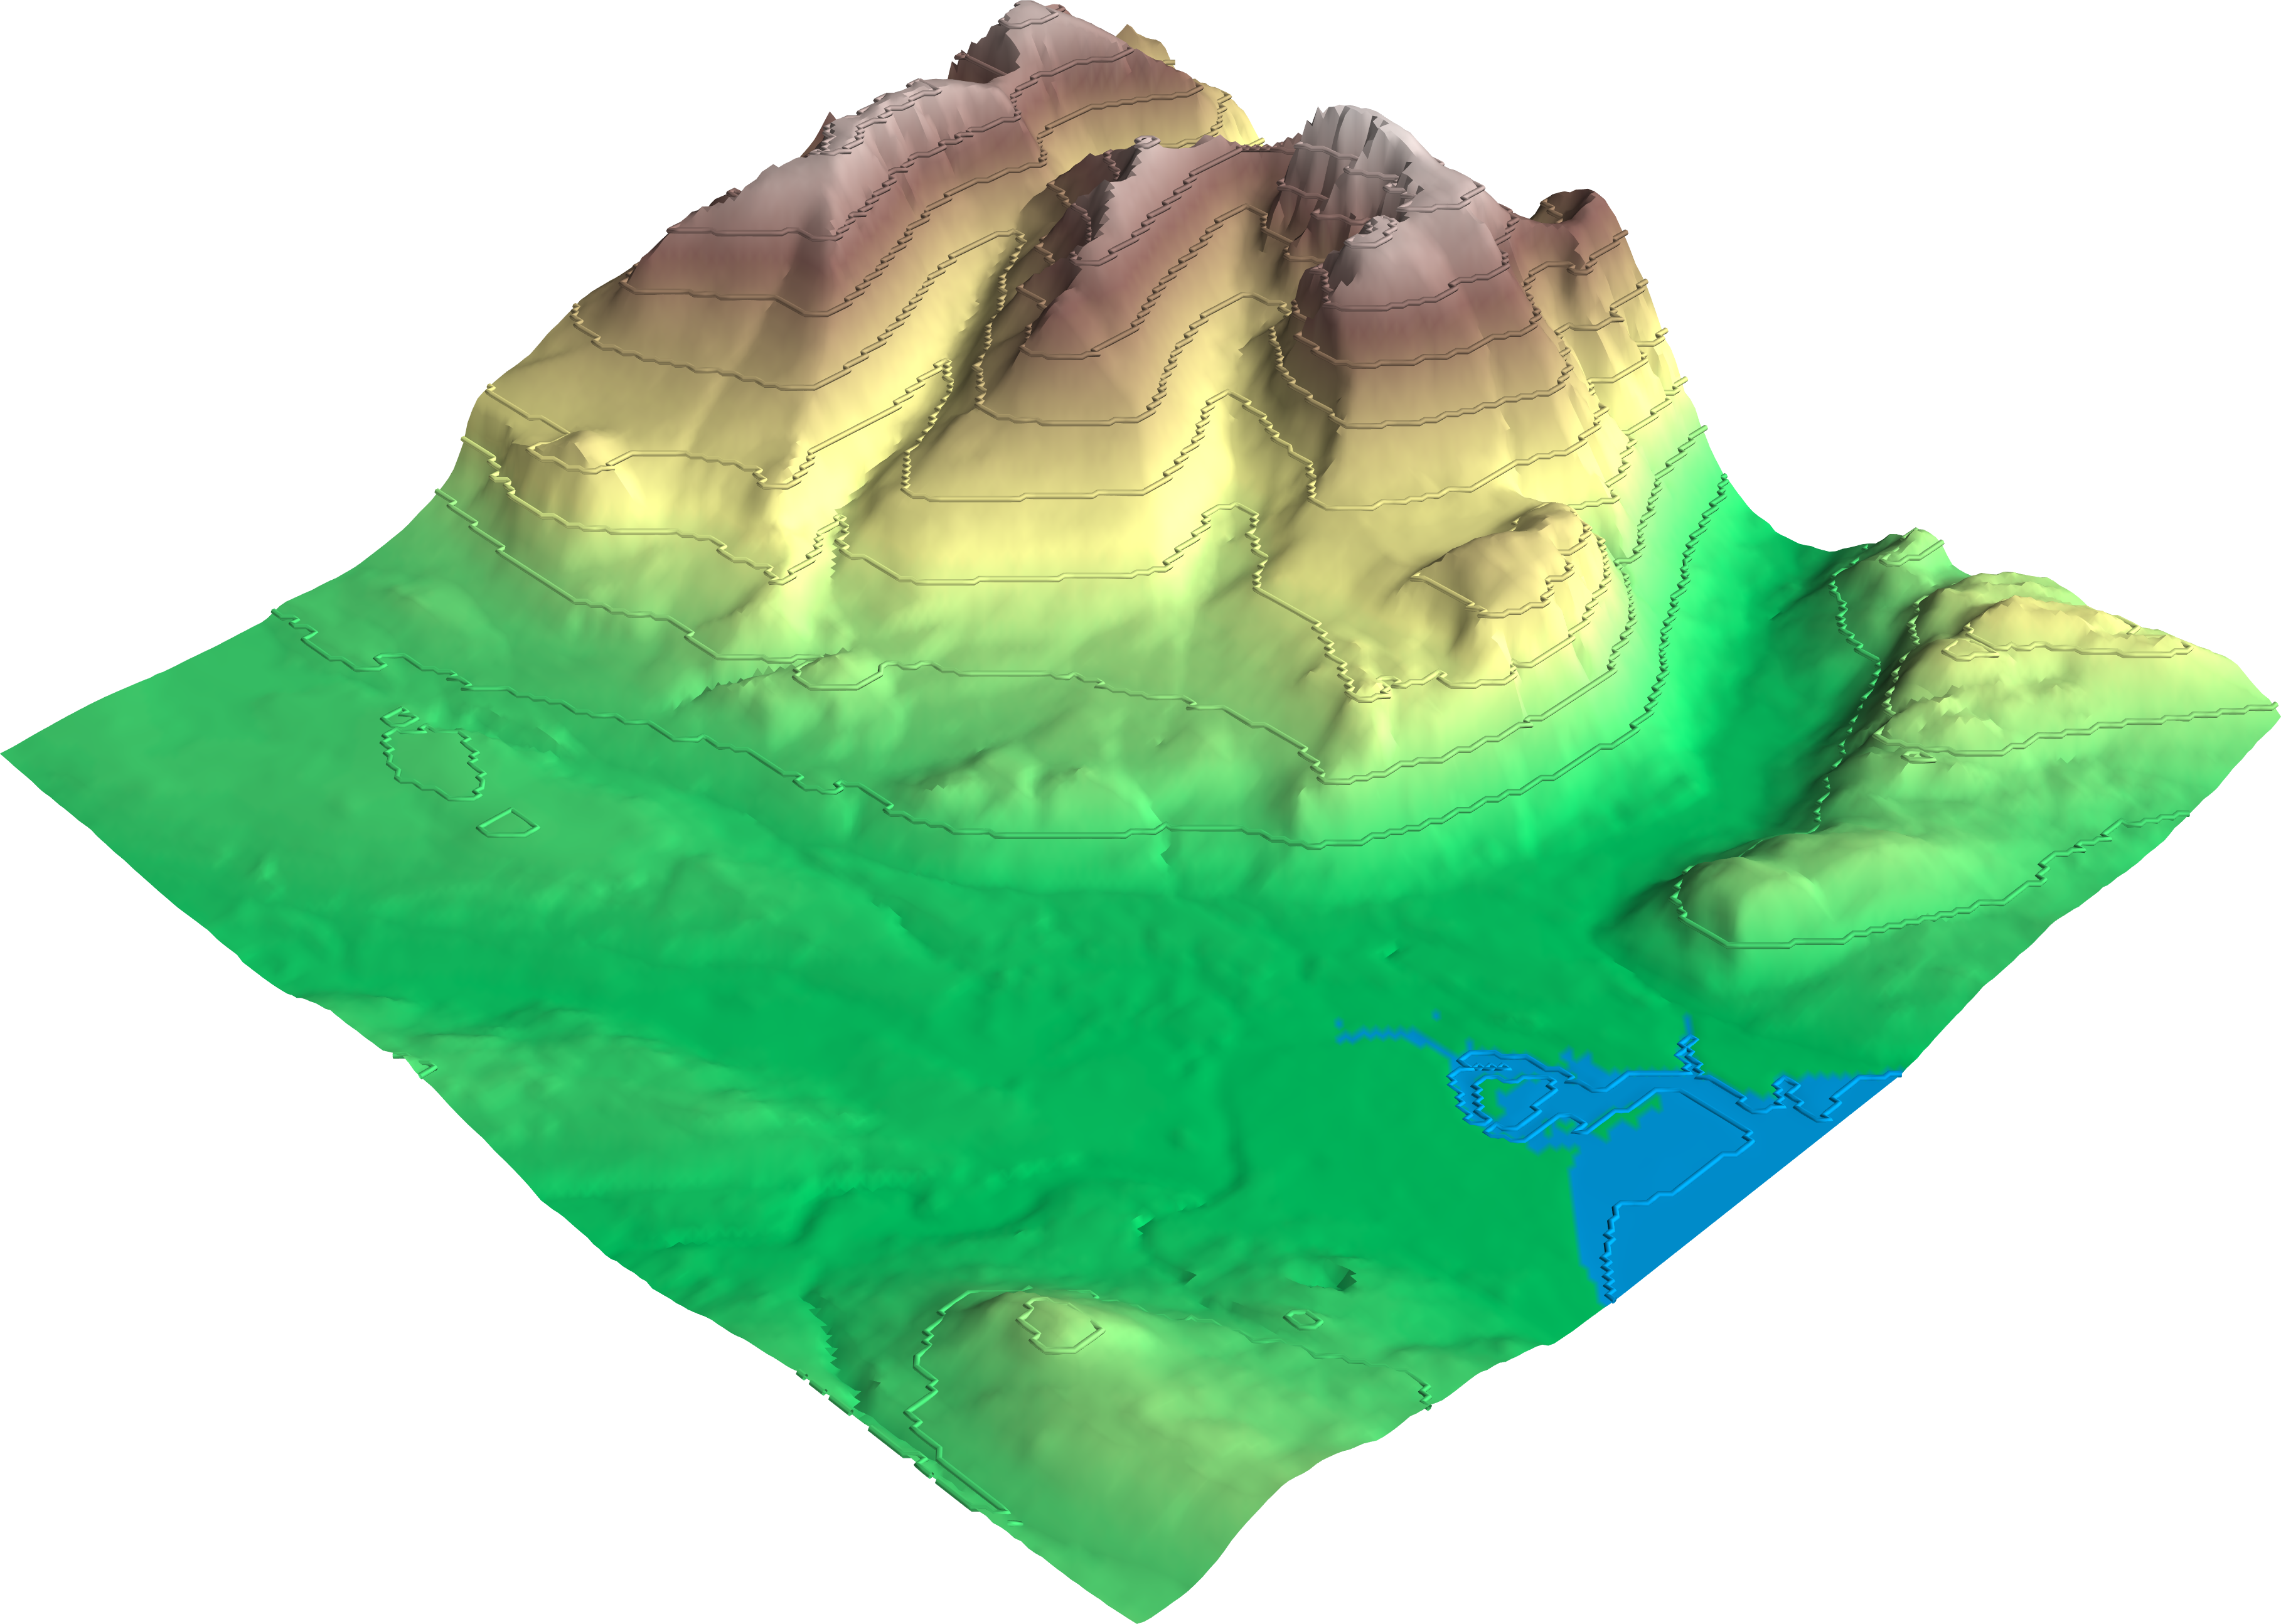
\includegraphics[width=1\textwidth]{../images/discretize/Accurate.png}
    \caption.{Accurate elevation surface with contours}
    \end{subfigure}
    \hfill
    \begin{subfigure}{.3\textwidth}
        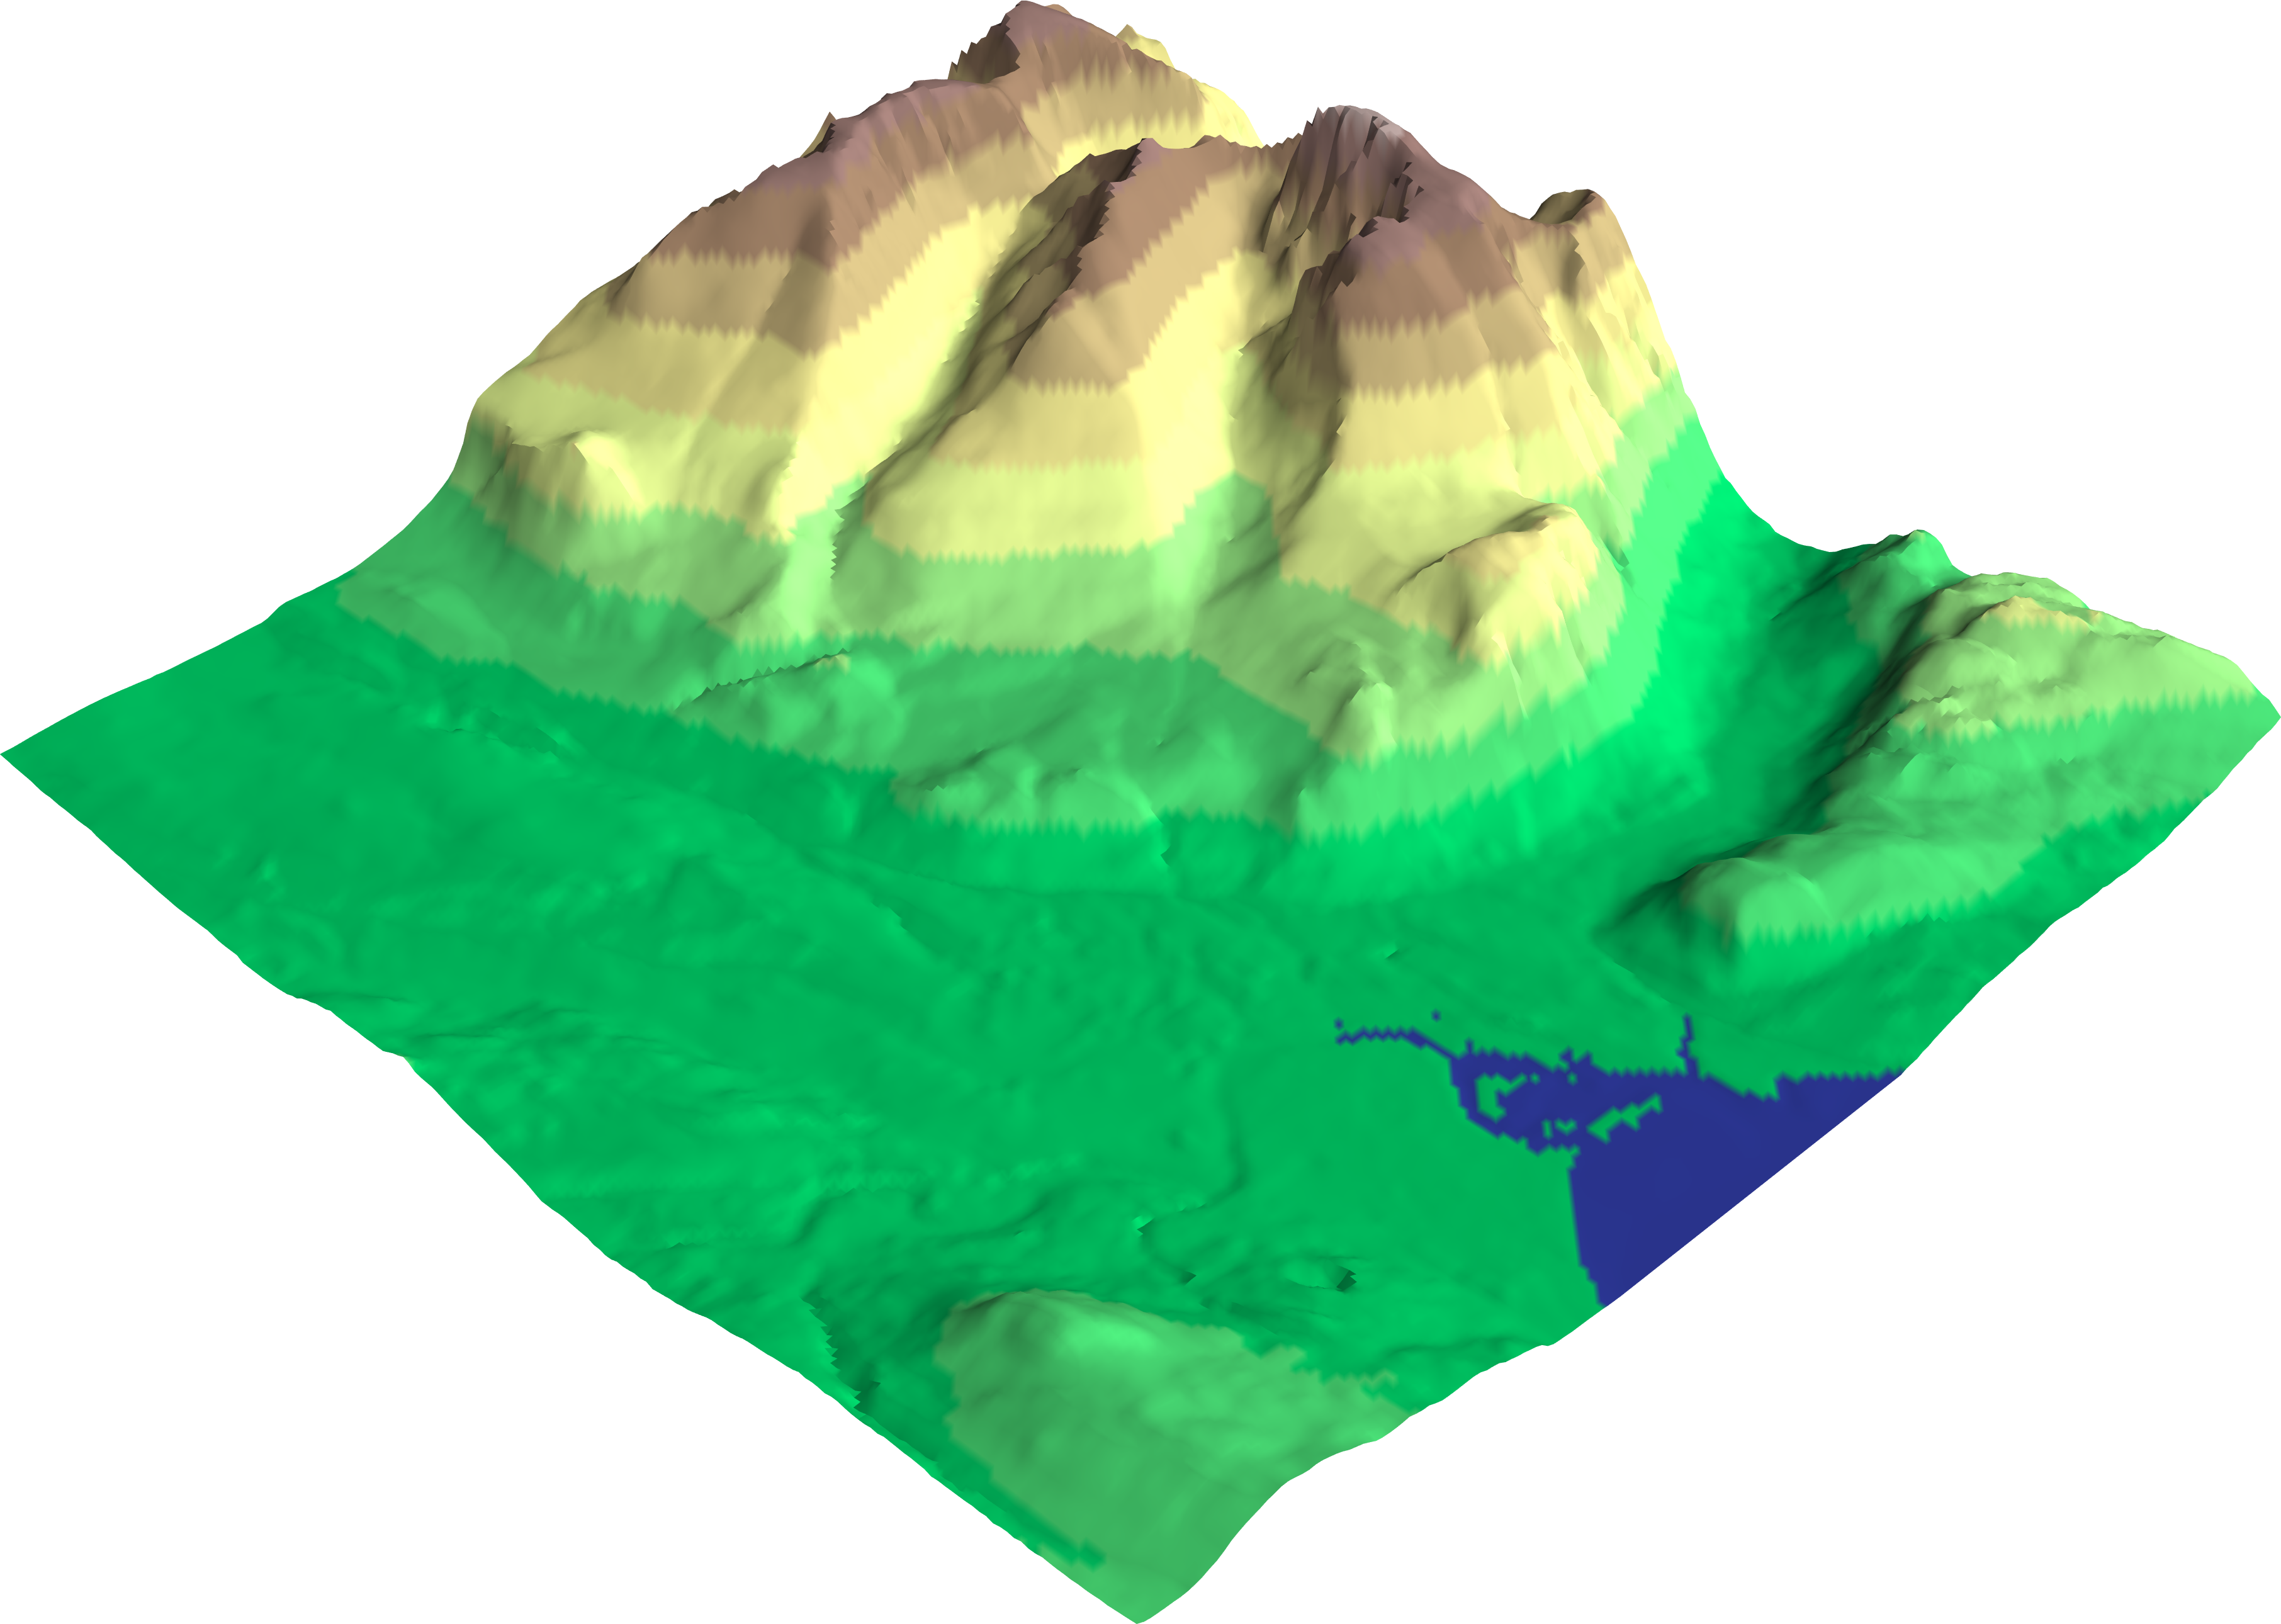
\includegraphics[width=1\textwidth]{../images/discretize/Color_Graded.png}
    \caption{Accurate elevation surface with colours graded according to discretization levels.}
    \end{subfigure}
    \hfill
    \begin{subfigure}{.3\textwidth}
        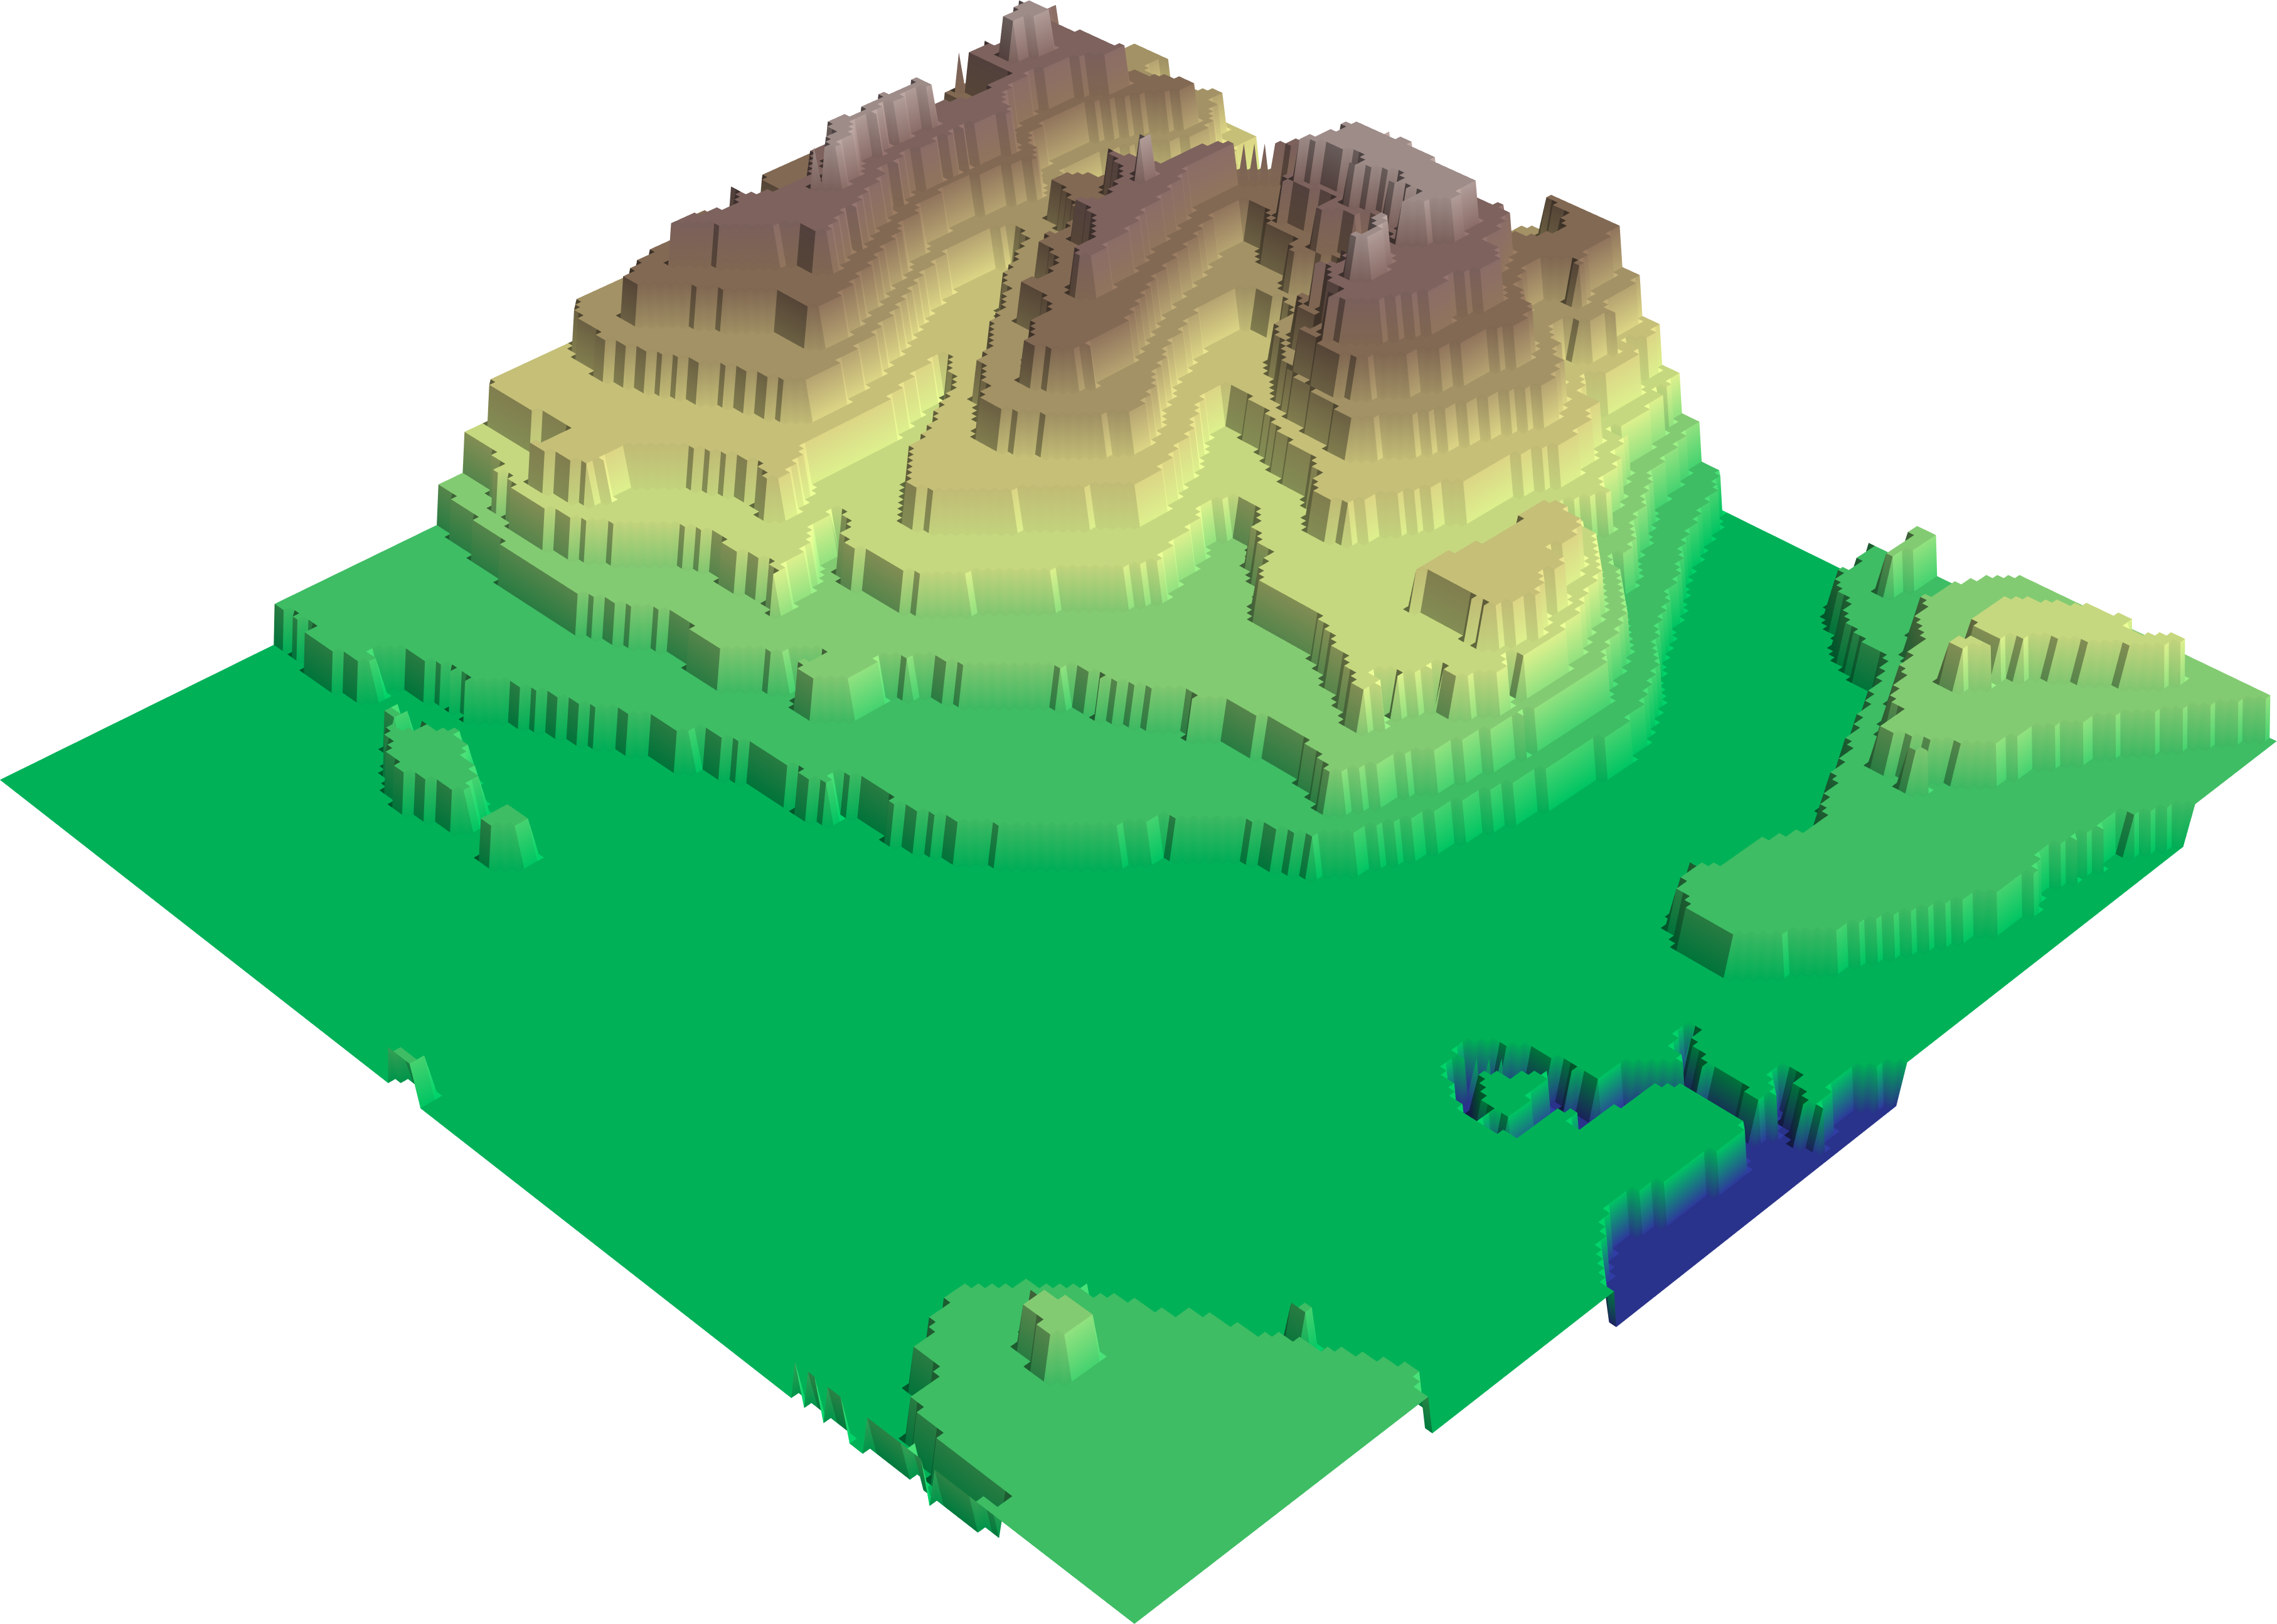
\includegraphics[width=1\textwidth]{../images/discretize/Discretized.png}
    \caption{Discretized elevation surface.}
    \end{subfigure}
    \caption{An example of discretization of elevation data from Fort William (UK ordnance tile NN17), northwest view.}
    \label{fig:3D_discrete_example}
\end{figure}

In the case where the domain is sampled sparsely, but is still on a regular grid, using bivariate spline interpolation is one of the fastest and most reliable methods to interpolate the data. We've used bicubic interpolation when interpolating DEMs in our examples, but in other cases using other degrees of polynomials is also valid and the choice should perhaps be motivated by the problem.

Analogously to 1D, interpolating a discretized image of a function requires us to pre-process the data and isolate some subset of points. This is perhaps a step which depends on the nature of the data that we are trying to interpolate.

In the case of our  DEM examples, we assume that in a discretized DEM, a particular value represents real height which is equal or higher than the value. In other words, the discretized values were created by rounding down to the nearest level. Therefore, the only real values truly preserved by the discretized data representation is located on the curves where two coplanar regions meet - on the contour lines. The elevation level of the contour is then determined by the higher value of the two coplanar regions.

By isolating contours from the discretized data we obtain a set of irregularly spaced points in the domain. Using bicubic interpolation therefore is not a valid option, as that requires a regular grid. There are two alternative methods we investigate in this report. One uses Delaunay triangulation to produce a triangular mesh from the isolated points, and then uses either barycentric interpolation or Clough-Tocher scheme (which in turn uses piecewise cubic interpolating Bézier polynomials). Other option is to use radial basis function (RBF) interpolation.

A radial basis function is a real-valued univariate function of the form $\varphi(||\mathbf{x}-\mathbf{c}||)$. The RBF interpolating function $s(\mathbf{x})$ is formed from the weighted sum of radial basis functions, one for each point $\mathbf{x}_k$ from the data that is being interpolated. The weights $w_k$ are chosen such that $\forall k:\ s(\mathbf{x}_k)=f(\mathbf{x}_k)$, i.e. $s(\mathbf{x})$ interpolates the original function $f(\mathbf{x})$ at the original points $\mathbf{x}_k$ with zero error.\footnote{\url{https://en.wikipedia.org/wiki/Radial\_basis\_function\_interpolation\#Examples}}
$$
s(x) = \sum\limits_{k} w_k \varphi(\|\mathbf{x}-\mathbf{x}_k\|)
$$
\begin{equation*}
 \begin{bmatrix}
\varphi(\|\mathbf{x}_0 - \mathbf{x}_0\|) & \varphi(\|\mathbf{x}_1 - \mathbf{x}_0\|) & \dots & \varphi(\|\mathbf{x}_{14} - \mathbf{x}_0\|) \\
\varphi(\|\mathbf{x}_0 - \mathbf{x}_1\|) & \varphi(\|\mathbf{x}_1 - \mathbf{x}_1\|) & \dots & \varphi(\|\mathbf{x}_{14} - \mathbf{x}_{1}\|) \\
\vdots & \vdots & \ddots & \vdots \\
\varphi(\|\mathbf{x}_0 - \mathbf{x}_{14}\|) & \varphi(\|\mathbf{x}_1 - \mathbf{x}_{14}\|) & \dots & \varphi(\|\mathbf{x}_{14} - \mathbf{x}_{14}\|) \\
\end{bmatrix}
\begin{bmatrix}w_0 \\ w_1 \\ \vdots \\ w_{14}\end{bmatrix}
= \begin{bmatrix}f(\mathbf{x}_0) \\ f(\mathbf{x}_1) \\ \vdots \\ f(\mathbf{x}_{14})\end{bmatrix}.
\end{equation*}
There is a degree of freedom in the choice of the RBF, some examples include linear $\varphi(r) = r$, thin plate spline $\varphi(r) = r^2\log{r}$, multiquadric $\varphi(r) = \sqrt{1+(\varepsilon r)^2}$ and many more.

\begin{figure}[H]
    \centering
    \begin{subfigure}{\textwidth}
        \includesvg[width=1\textwidth]{../images/differences/Delaunay_Triangulation_and_Barycentric_Interpolation_2D.svg}
        % 2D_Contour_Interpolation.svg: 1600x900 px, 100dpi, 40.64x22.86 cm, bb=0 0 1152 648
    \caption{Delaunay triangulation used together with barycentric interpolation.}
    \end{subfigure}
    \begin{subfigure}{\textwidth}
        \includesvg[width=1\textwidth]{../images/differences/Delaunay_Triangulation_and_Clough-Tocher_scheme_2D.svg}
        % 2D_Contour_Interpolation.svg: 1600x900 px, 100dpi, 40.64x22.86 cm, bb=0 0 1152 648
    \caption{Delaunay triangulation used together with Clough-Tocher scheme.}
    \end{subfigure}
    \begin{subfigure}{\textwidth}
        \includesvg[width=1\textwidth]{../images/differences/Radial_Basis_Thin_Plate_Spline_2D.svg}
        % 2D_Contour_Interpolation.svg: 1600x900 px, 100dpi, 40.64x22.86 cm, bb=0 0 1152 648
    \caption{Radial basis function interpolation using thin plate spline radial function.}
    \end{subfigure}
    \caption{Comparison of various interpolation methods using elevation data from UK ordnance tile NO44 (South of Forfar).}
    \label{fig:2D_discretized_comparison}
\end{figure}

\begin{figure}[H]
    \centering
    \begin{subfigure}{.32\textwidth}
        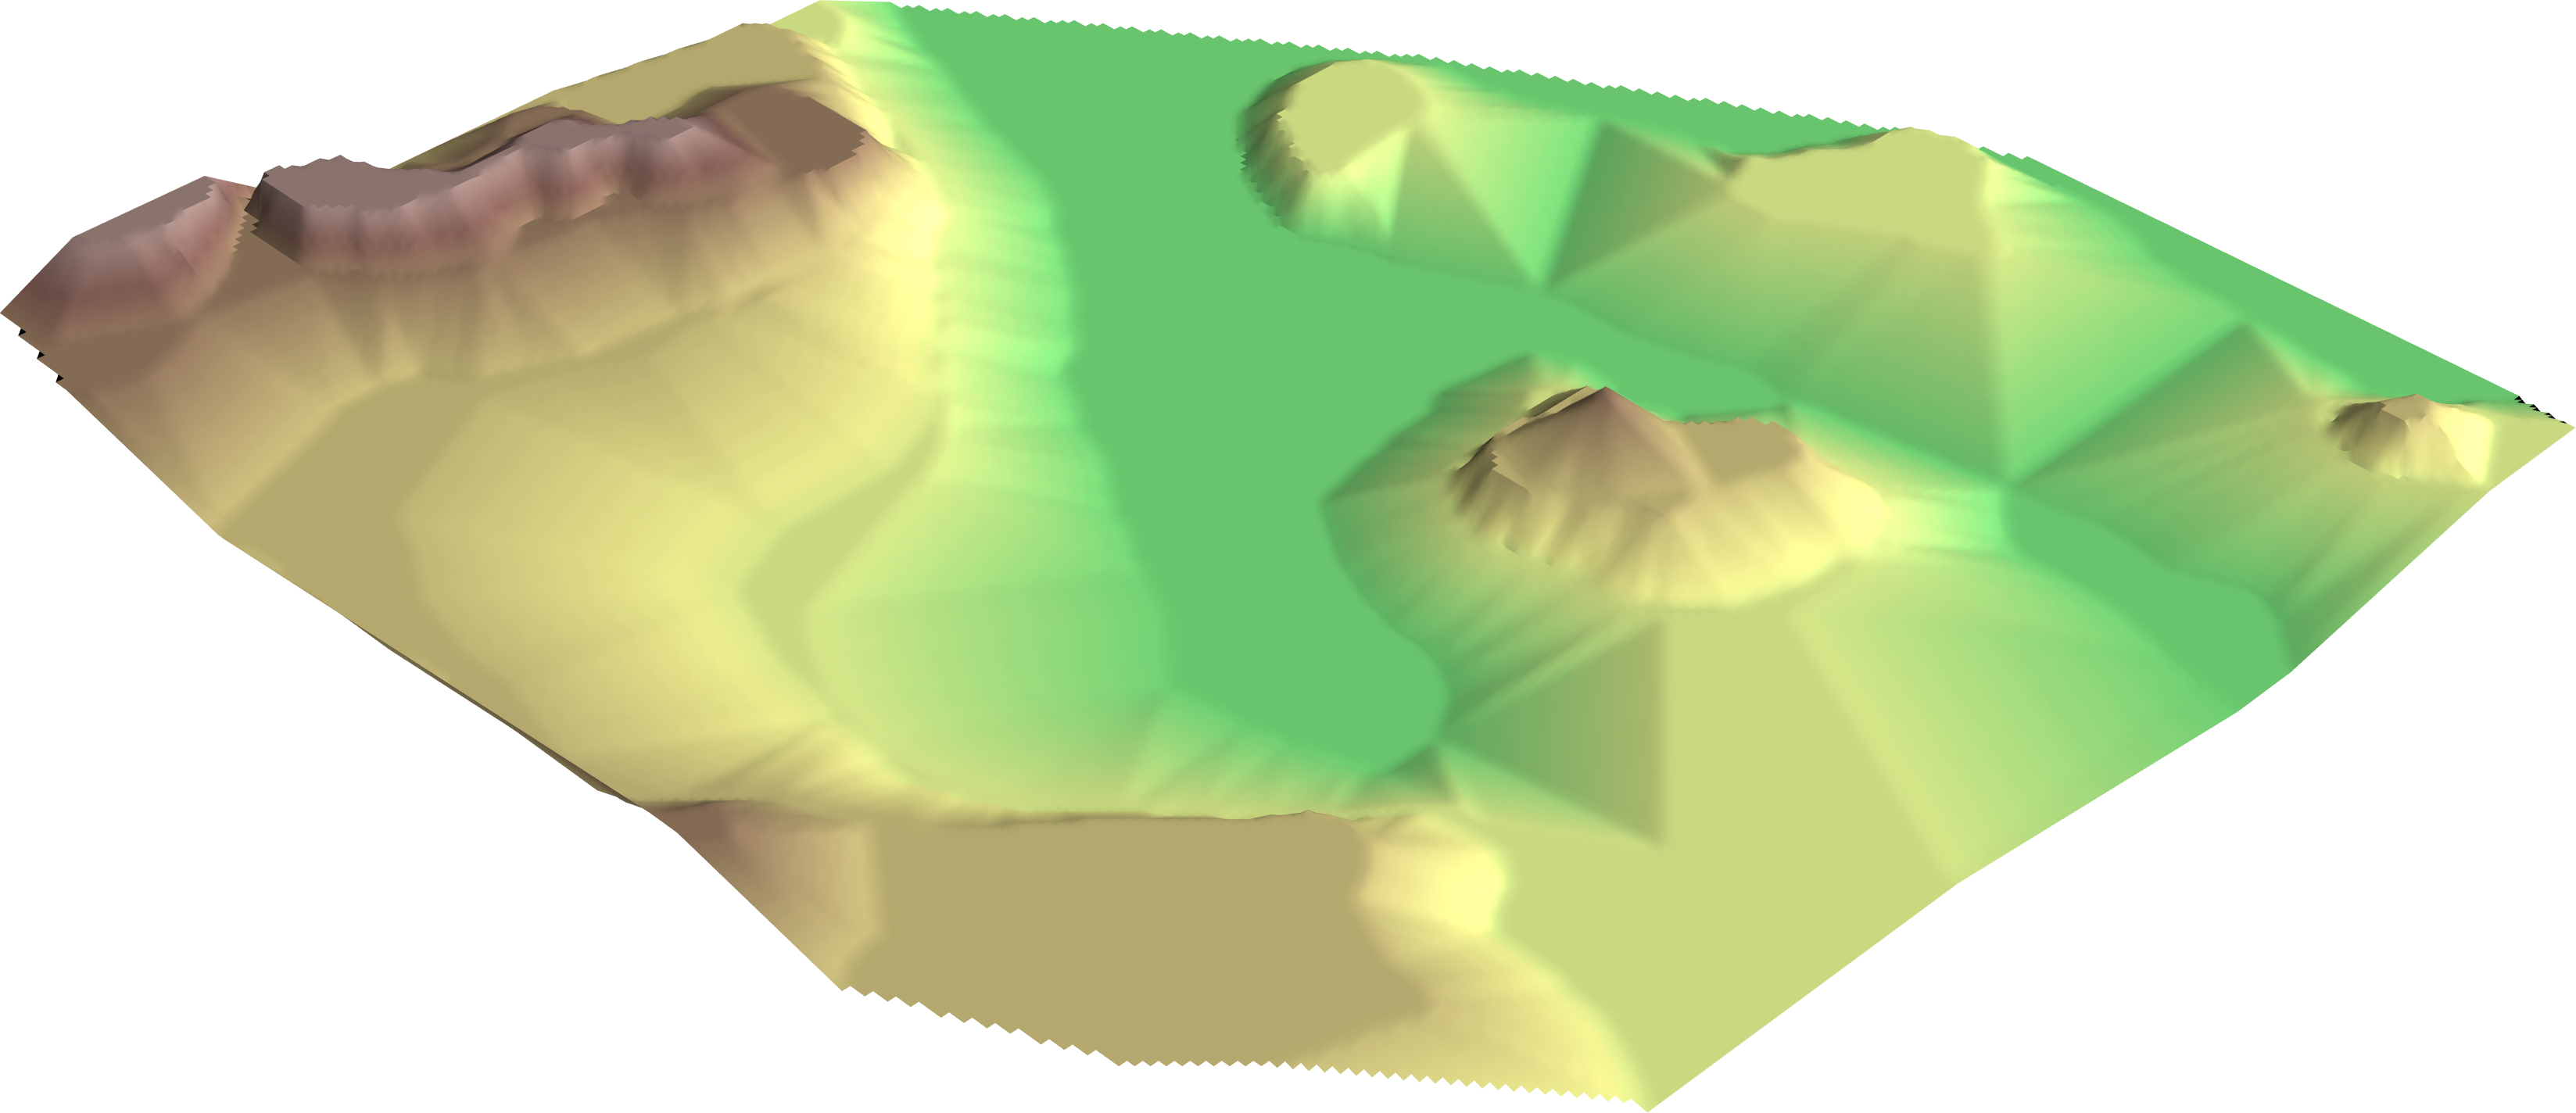
\includegraphics[width=\textwidth]{../images/differences/Delaunay_Triangulation_and_Barycentric_Interpolation_3D.png}
        % 2D_Contour_Interpolation.png: 1600x900 px, 100dpi, 40.64x22.86 cm, bb=0 0 1152 648
    \caption{Delaunay triangulation used together with barycentric interpolation.}
    \label{fig:3D_discretized_comparison_a}
    \end{subfigure}
    \hfill
    \begin{subfigure}{.32\textwidth}
        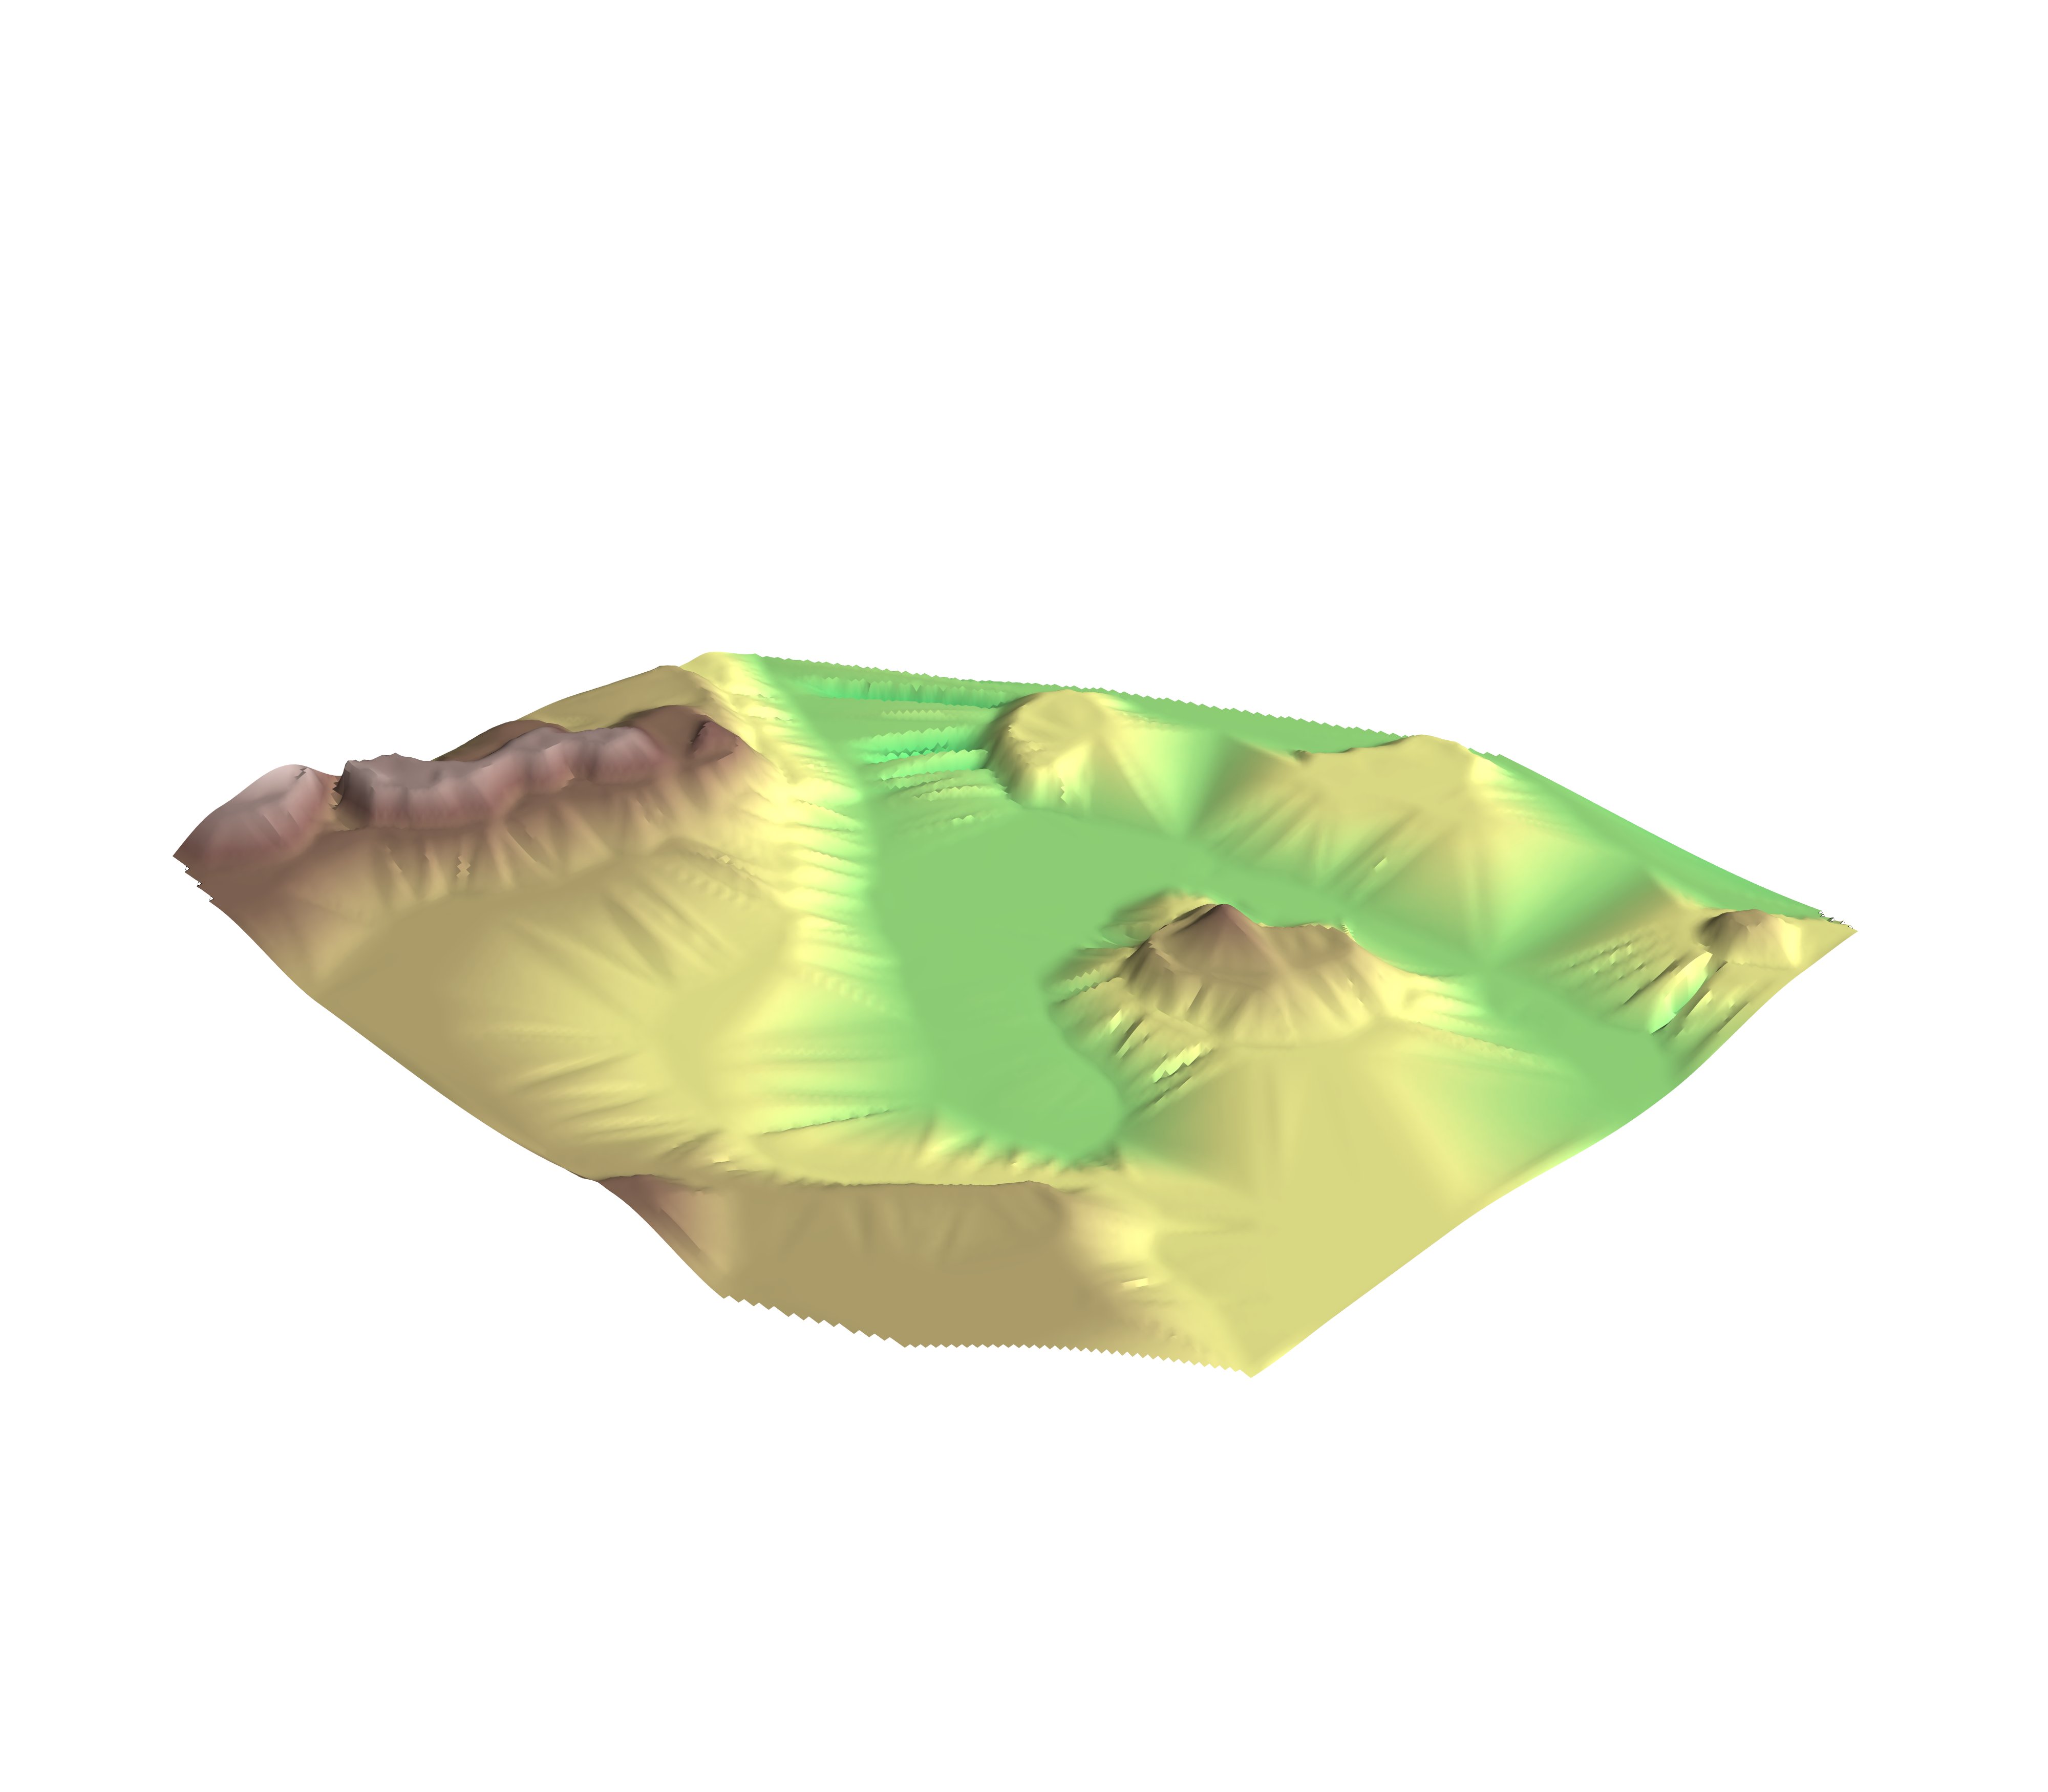
\includegraphics[width=\textwidth]{../images/differences/Delaunay_Triangulation_and_Clough-Tocher_scheme_3D.png}
        % 2D_Contour_Interpolation.png: 1600x900 px, 100dpi, 40.64x22.86 cm, bb=0 0 1152 648
    \caption{Delaunay triangulation used together with Clough-Tocher scheme.}
    \label{fig:3D_discretized_comparison_b}
    \end{subfigure}
    \hfill
    \begin{subfigure}{.32\textwidth}
        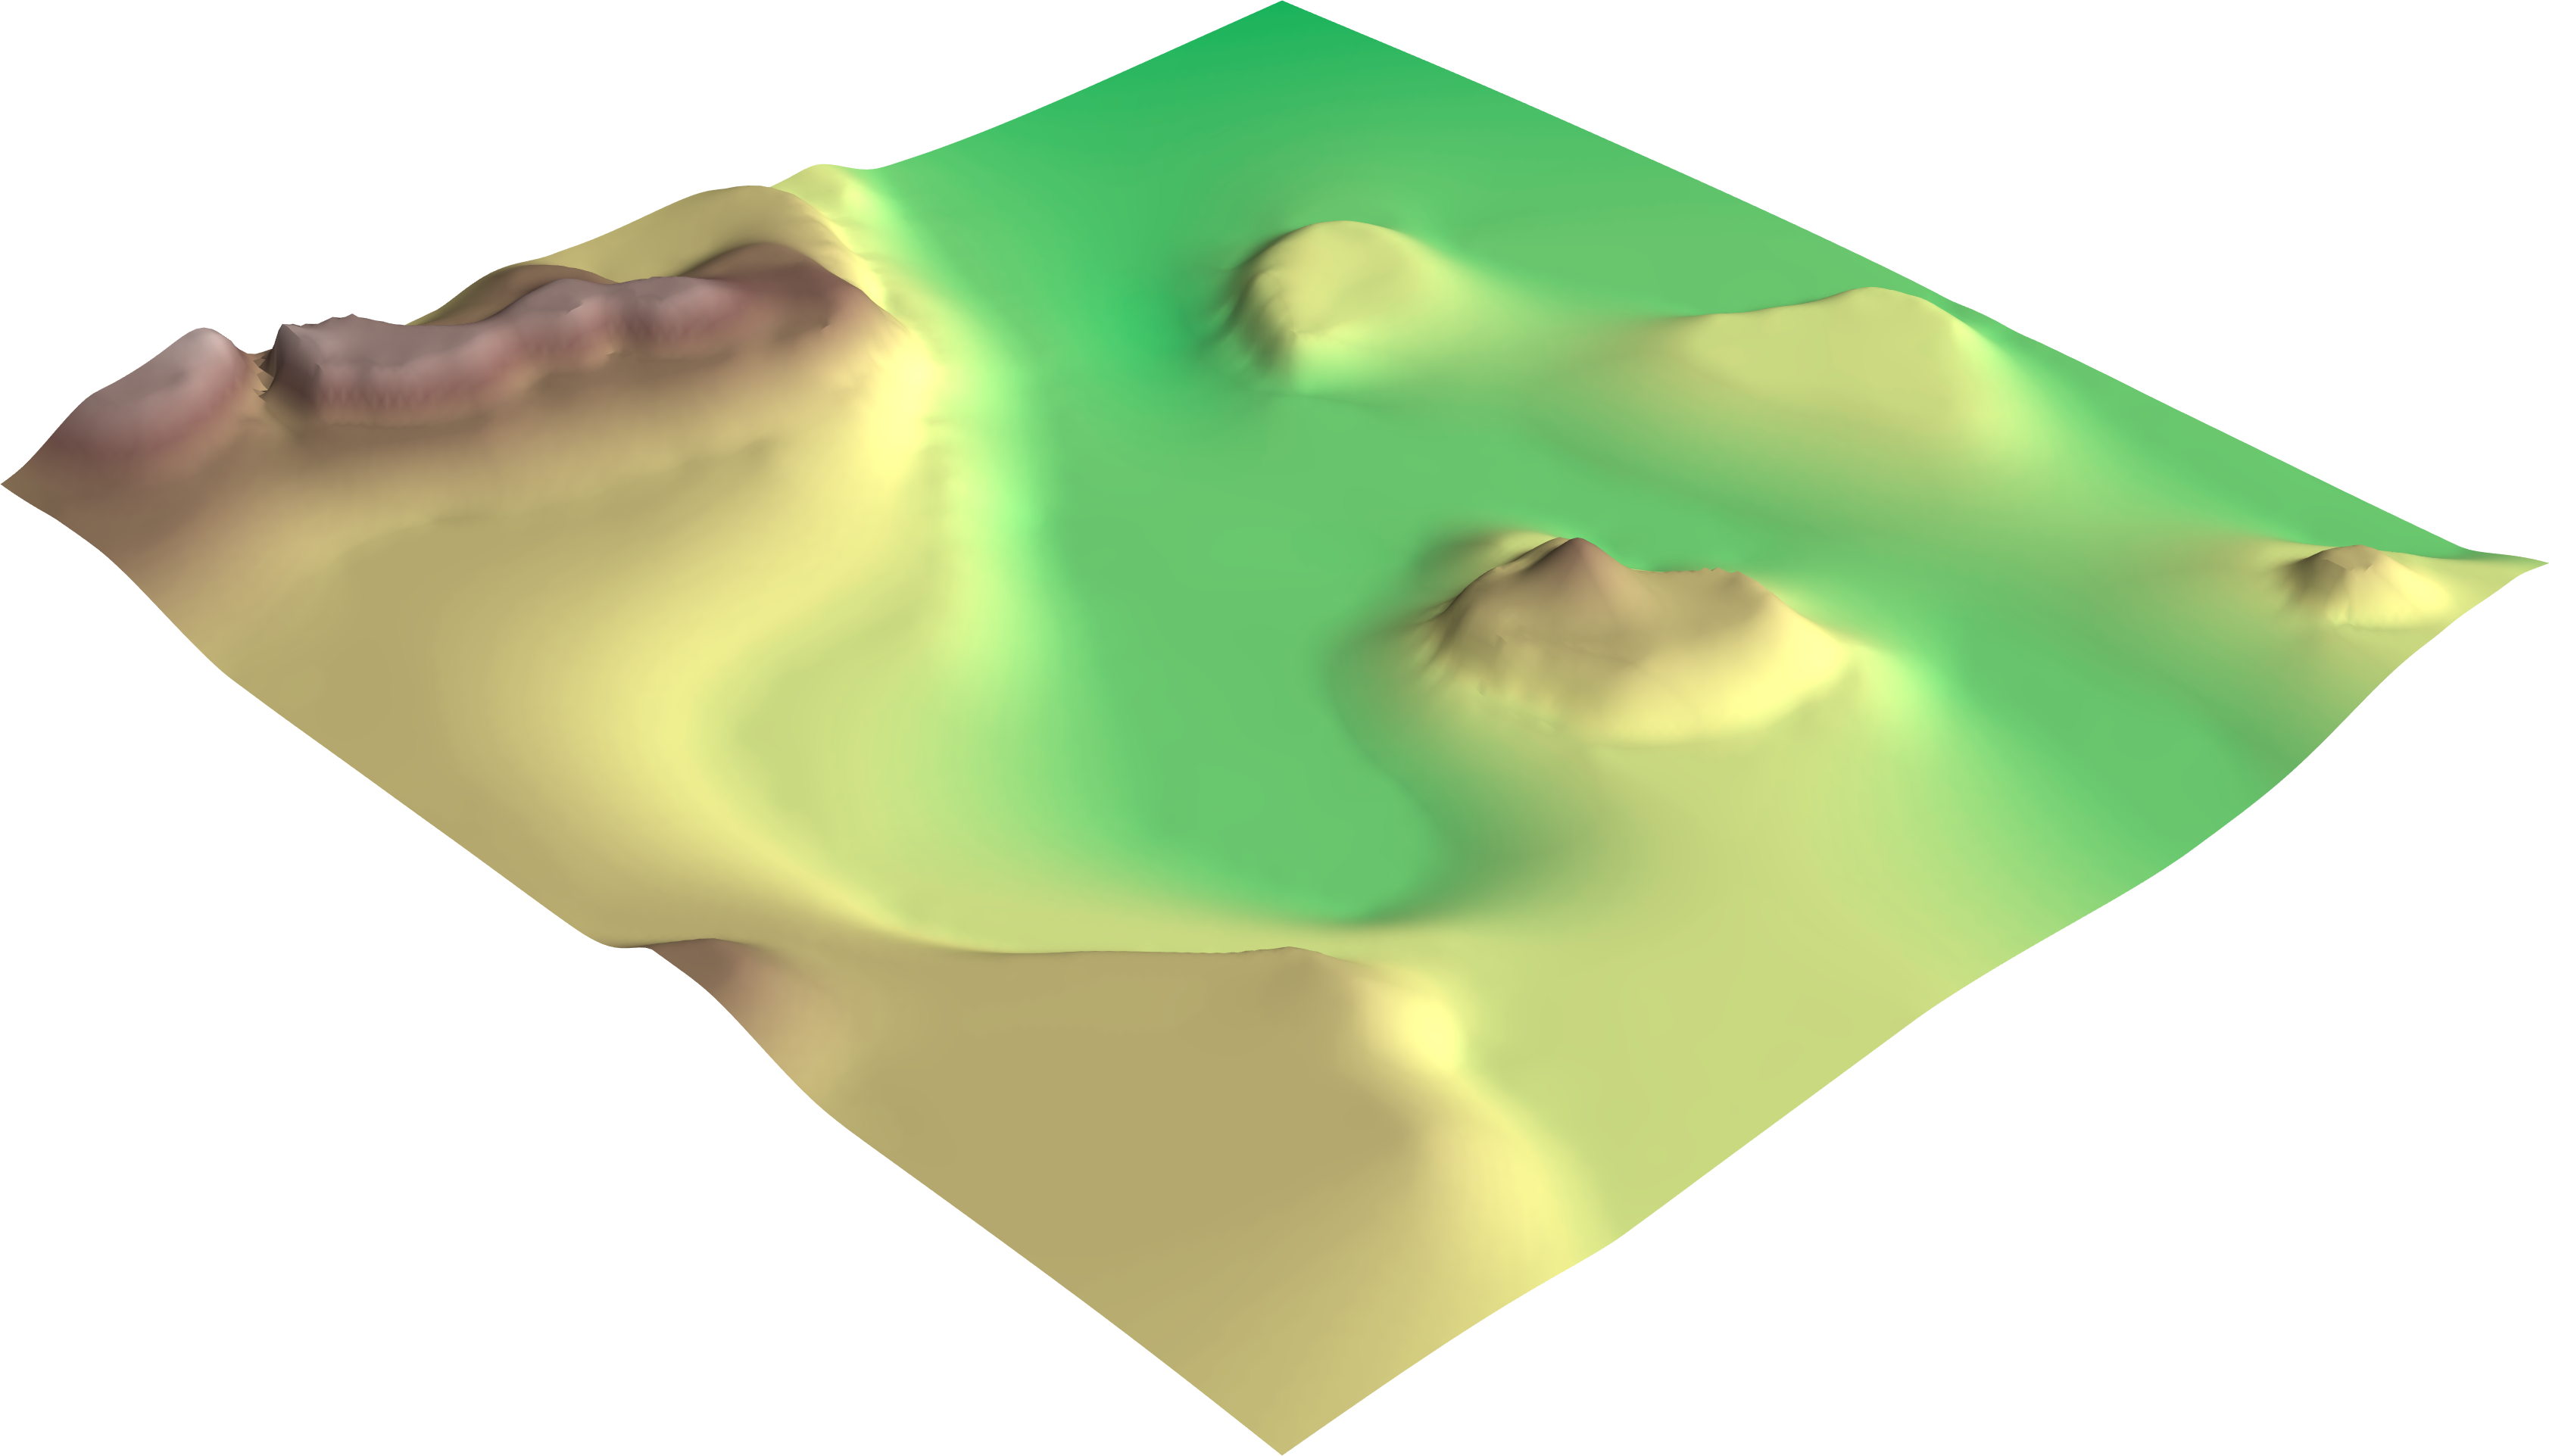
\includegraphics[width=\textwidth]{../images/differences/Radial_Basis_Thin_Plate_Spline_3D.png}
        % 2D_Contour_Interpolation.png: 1600x900 px, 100dpi, 40.64x22.86 cm, bb=0 0 1152 648
    \caption{Radial basis function interpolation using thin plate spline radial function.}
    \label{fig:3D_discretized_comparison_c}
    \end{subfigure}
    \caption{Comparison of various interpolation methods using elevation data from UK ordnance tile NO44 (South of Forfar), southeast view.}
    \label{fig:3D_discretized_comparison}
\end{figure}

In Figure \ref{fig:2D_discretized_comparison} and \ref{fig:3D_discretized_comparison} we compare the two aforementioned methods. We can immediately notice that neither of the methods is particularly accurate at the regions where no contour lines are available, in this case the NW corner of the tile. The methods using Delaunay triangulation do not interpolate regions outside the convex hull of the isolated points at all, and radial basis function interpolation does produce reasonable estimates, but as can be seen on the right-most plot the absolute error in this region is still quite high. However, this is perhaps expected, as there simply isn't enough information to interpolate in the first place.

Another issue with the Delaunay triangulation is that it doesn't produce smooth surfaces. This can be easily seen in Figure \ref{fig:3D_discretized_comparison_a} and \ref{fig:3D_discretized_comparison_b}, where the triangles still remain visible when visualizing the surface. The Clough-Tocher scheme also introduces artefacts in forms of stretched valleys.

The disadvantages of Delaunay triangulation lead us to opting for the radial basis function interpolation for DEMs. With this approach, we also have a choice of kernel function for the interpolation. We compared several, such as linear, thin plate spline, cubic, quintic, multiquadric, inverse multiquadric, inverse quadratic and Gaussian.\footnote{All available within the \href{https://docs.scipy.org/doc/scipy/reference/generated/scipy.interpolate.RBFInterpolator.html}{RBFInterpolator class} of Python SciPy library.}. Out of these, linear, thin plate spline and multiquadric produced results with the smallest errors. We can see the RBF interpolation in action on Figure \ref{fig:2D_data} and \ref{fig:3D_discretized_interpolation}.

\begin{figure}[H]
    \centering
    \begin{subfigure}{\textwidth}
        \includesvg[width=1\textwidth]{../images/NH52/2D_Data_Interpolation.svg}
        % 2D_Contour_Interpolation.svg: 1600x900 px, 100dpi, 40.64x22.86 cm, bb=0 0 1152 648
    \caption{Elevation data from Drumnadrochit, Loch Ness (UK ordnance tile NH52).}
    \end{subfigure}
    \begin{subfigure}{\textwidth}
        \includesvg[width=1\textwidth]{../images/NO33/2D_Data_Interpolation.svg}
        % 2D_Contour_Interpolation.svg: 1600x900 px, 100dpi, 40.64x22.86 cm, bb=0 0 1152 648
    \caption{Elevation data from west Dundee (UK ordnance tile NO33).}
    \end{subfigure}
    \caption{Interpolation of elevation data with various resolution by using thin plate spline method.}
    \label{fig:2D_data}
\end{figure}

\begin{figure}[H]
    \centering
    \begin{subfigure}{\textwidth}
        \begin{subfigure}{.49\textwidth}
        \centering
            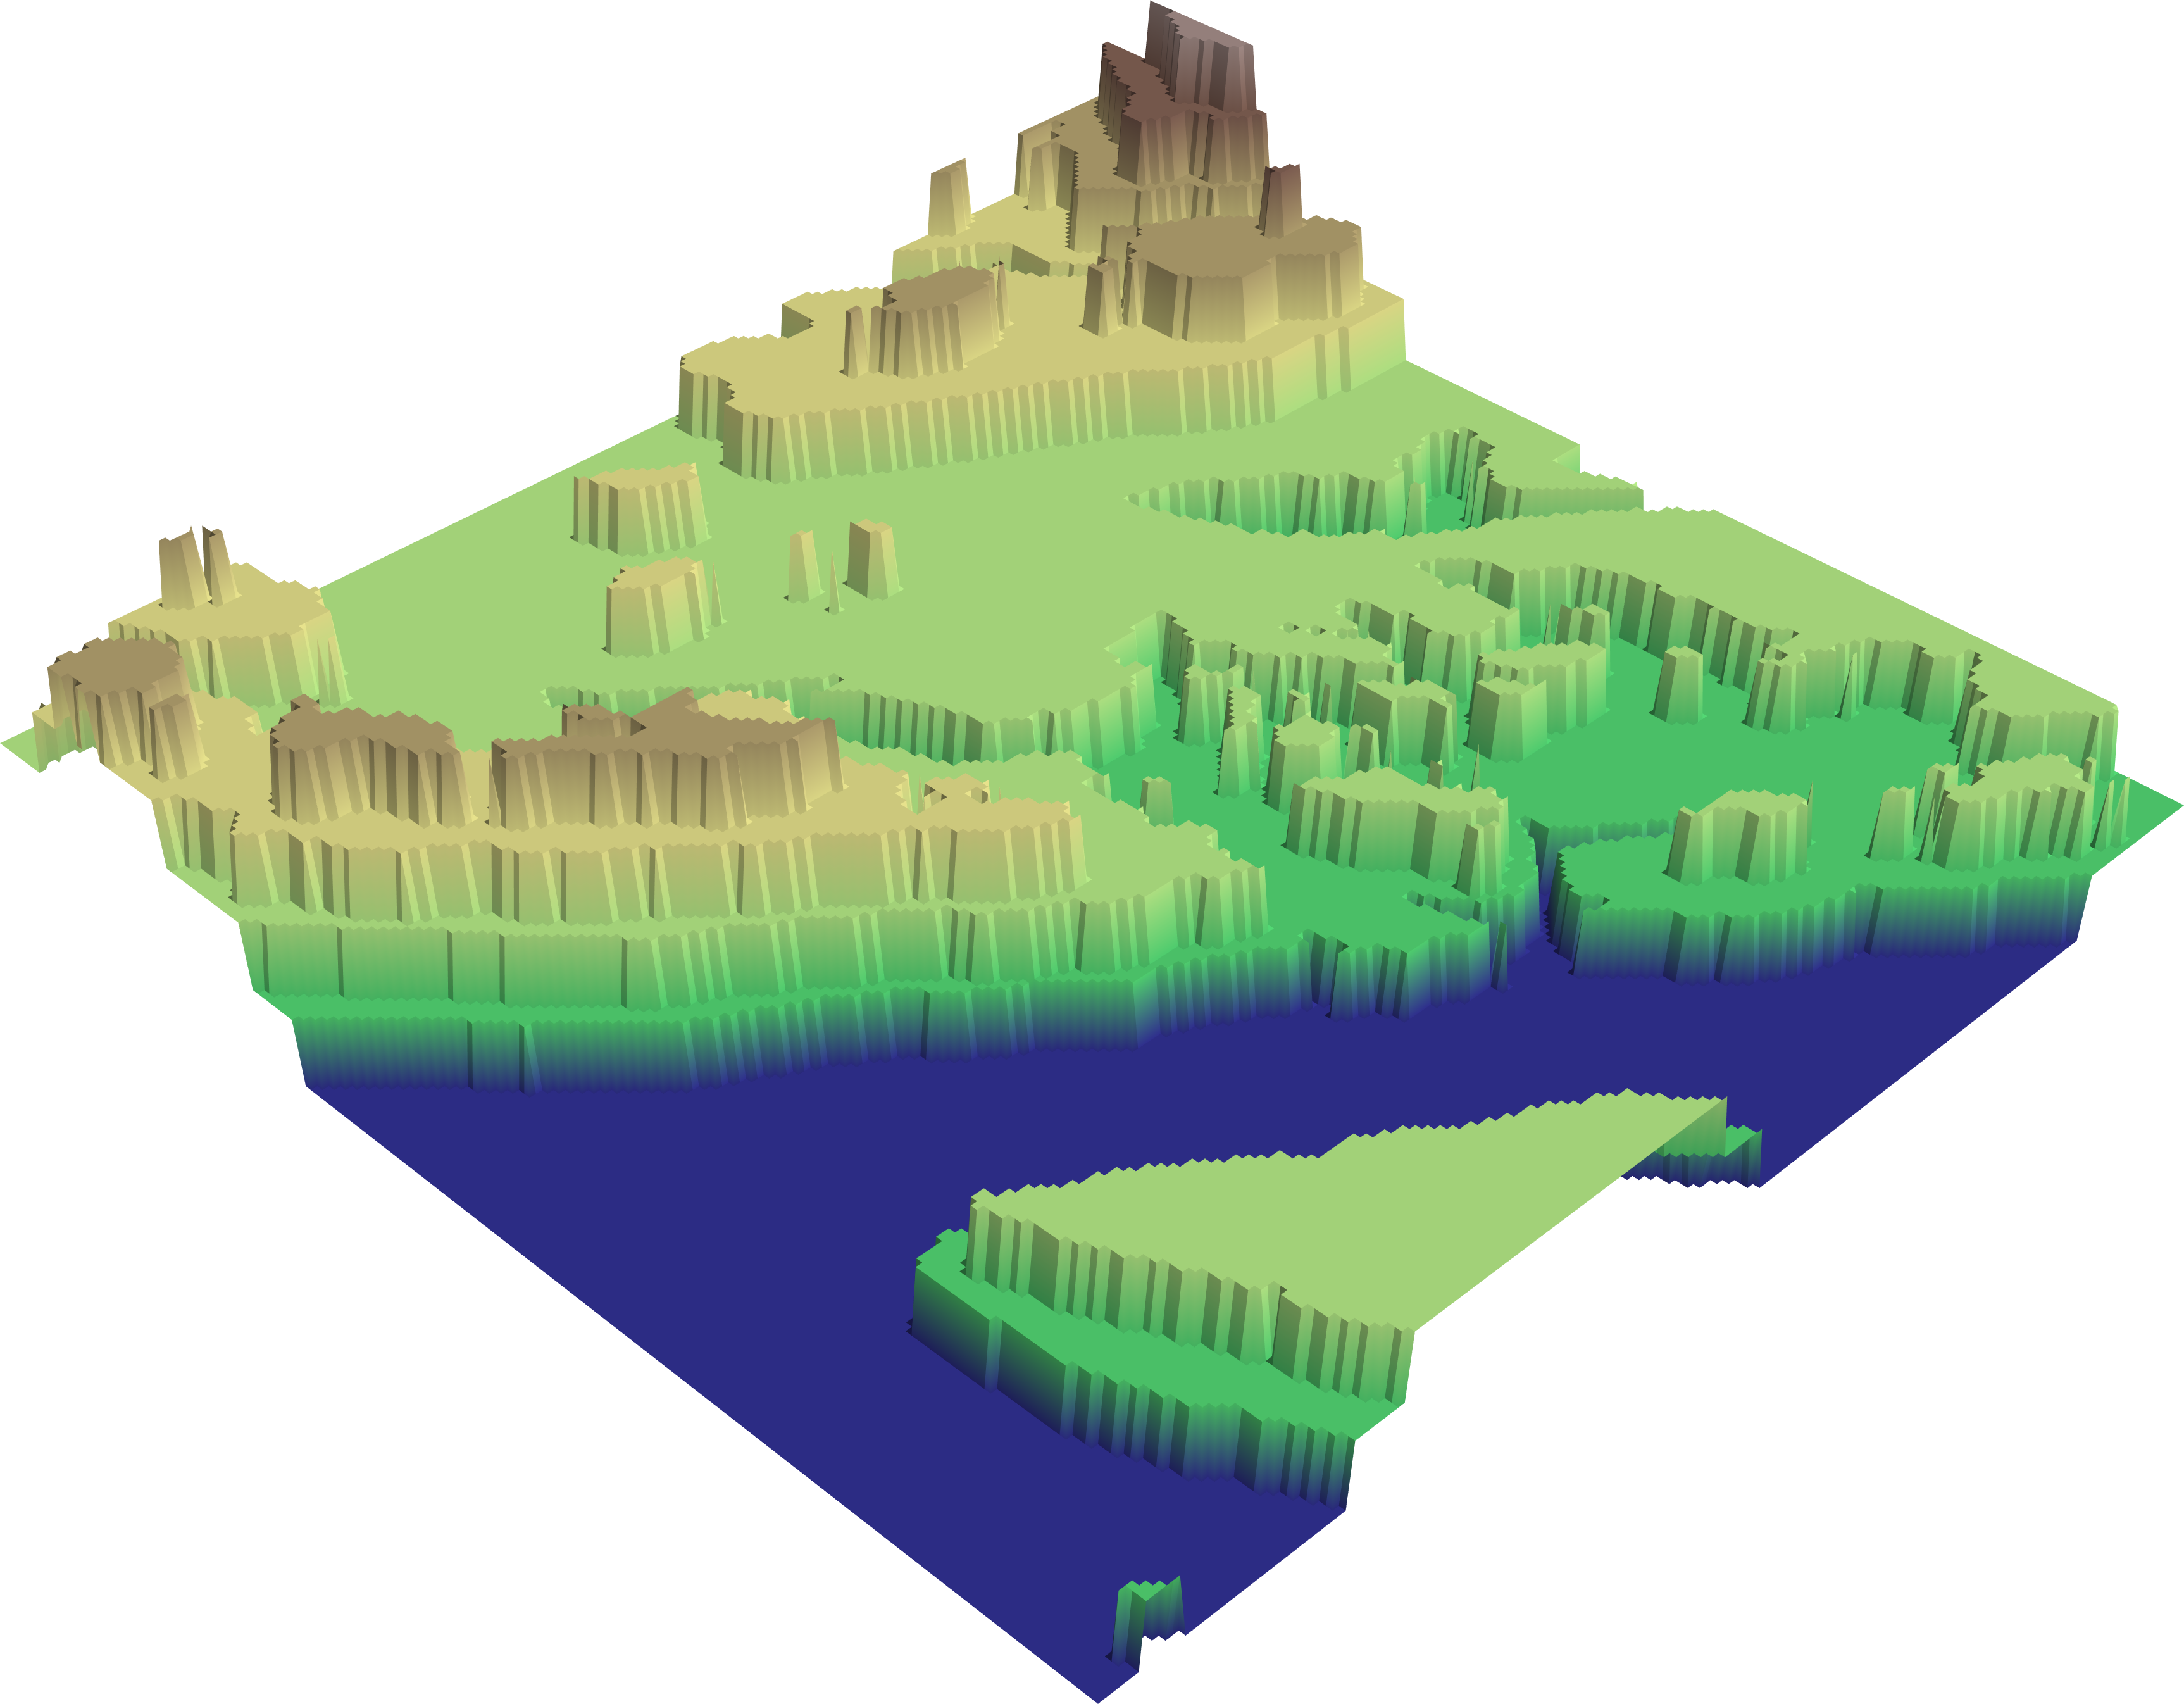
\includegraphics[width=\textwidth]{../images/NH52/2D_Data_Interpolation_3D_discretized_datagrid.png}
        \renewcommand\thesubfigure{\alph{subfigure}) i}
        \caption{Surface from discretized elevation data.}
        \end{subfigure}
        \hfill
        \begin{subfigure}{.49\textwidth}
            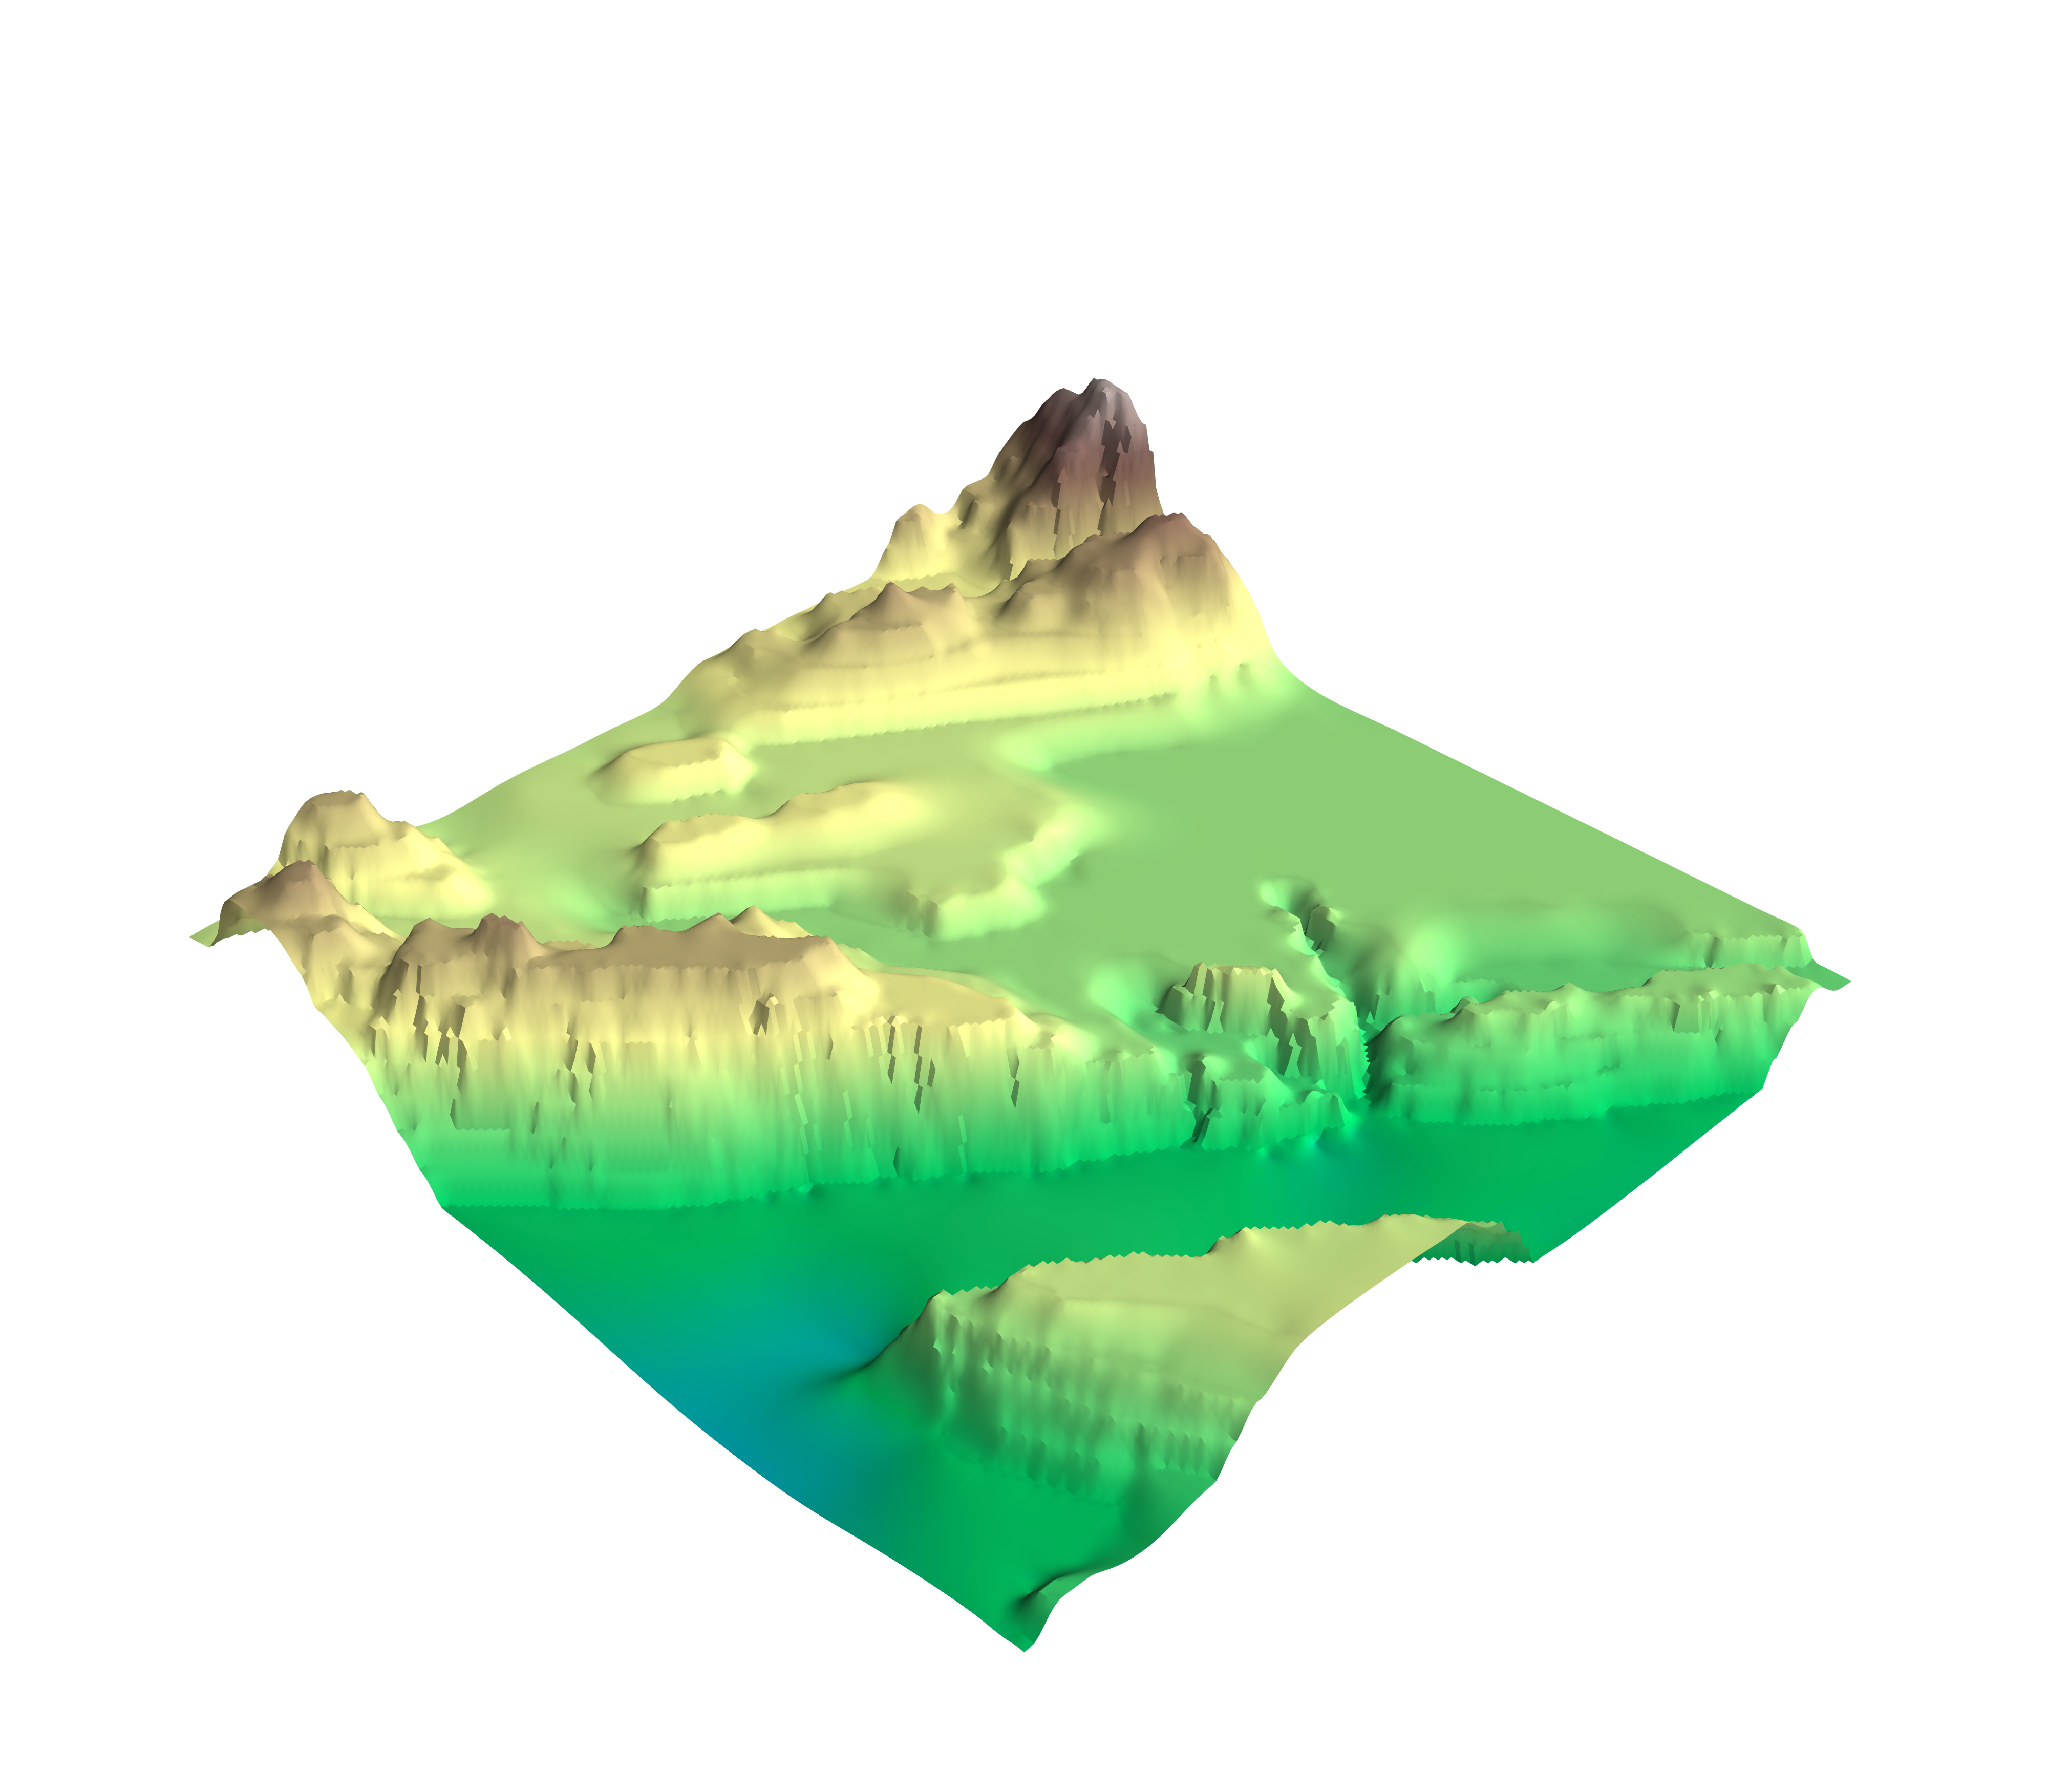
\includegraphics[width=\textwidth]{../images/NH52/2D_Data_Interpolation_3D_discretized_datagrid_interpolated.png}
        \addtocounter{subfigure}{-1}
        \renewcommand\thesubfigure{\alph{subfigure}) ii}
        \caption{Surface from interpolated elevation data.}
        \end{subfigure}
        \addtocounter{subfigure}{-1}
        \renewcommand\thesubfigure{\alph{subfigure}}
        \caption{Elevation data from Drumnadrochit, Loch Ness (UK ordnance tile NH52), northwest view.}
        \label{fig:3D_discretized_interpolation_a}
    \end{subfigure}
    \begin{subfigure}{\textwidth}
        \centering
        \begin{subfigure}{.49\textwidth}
            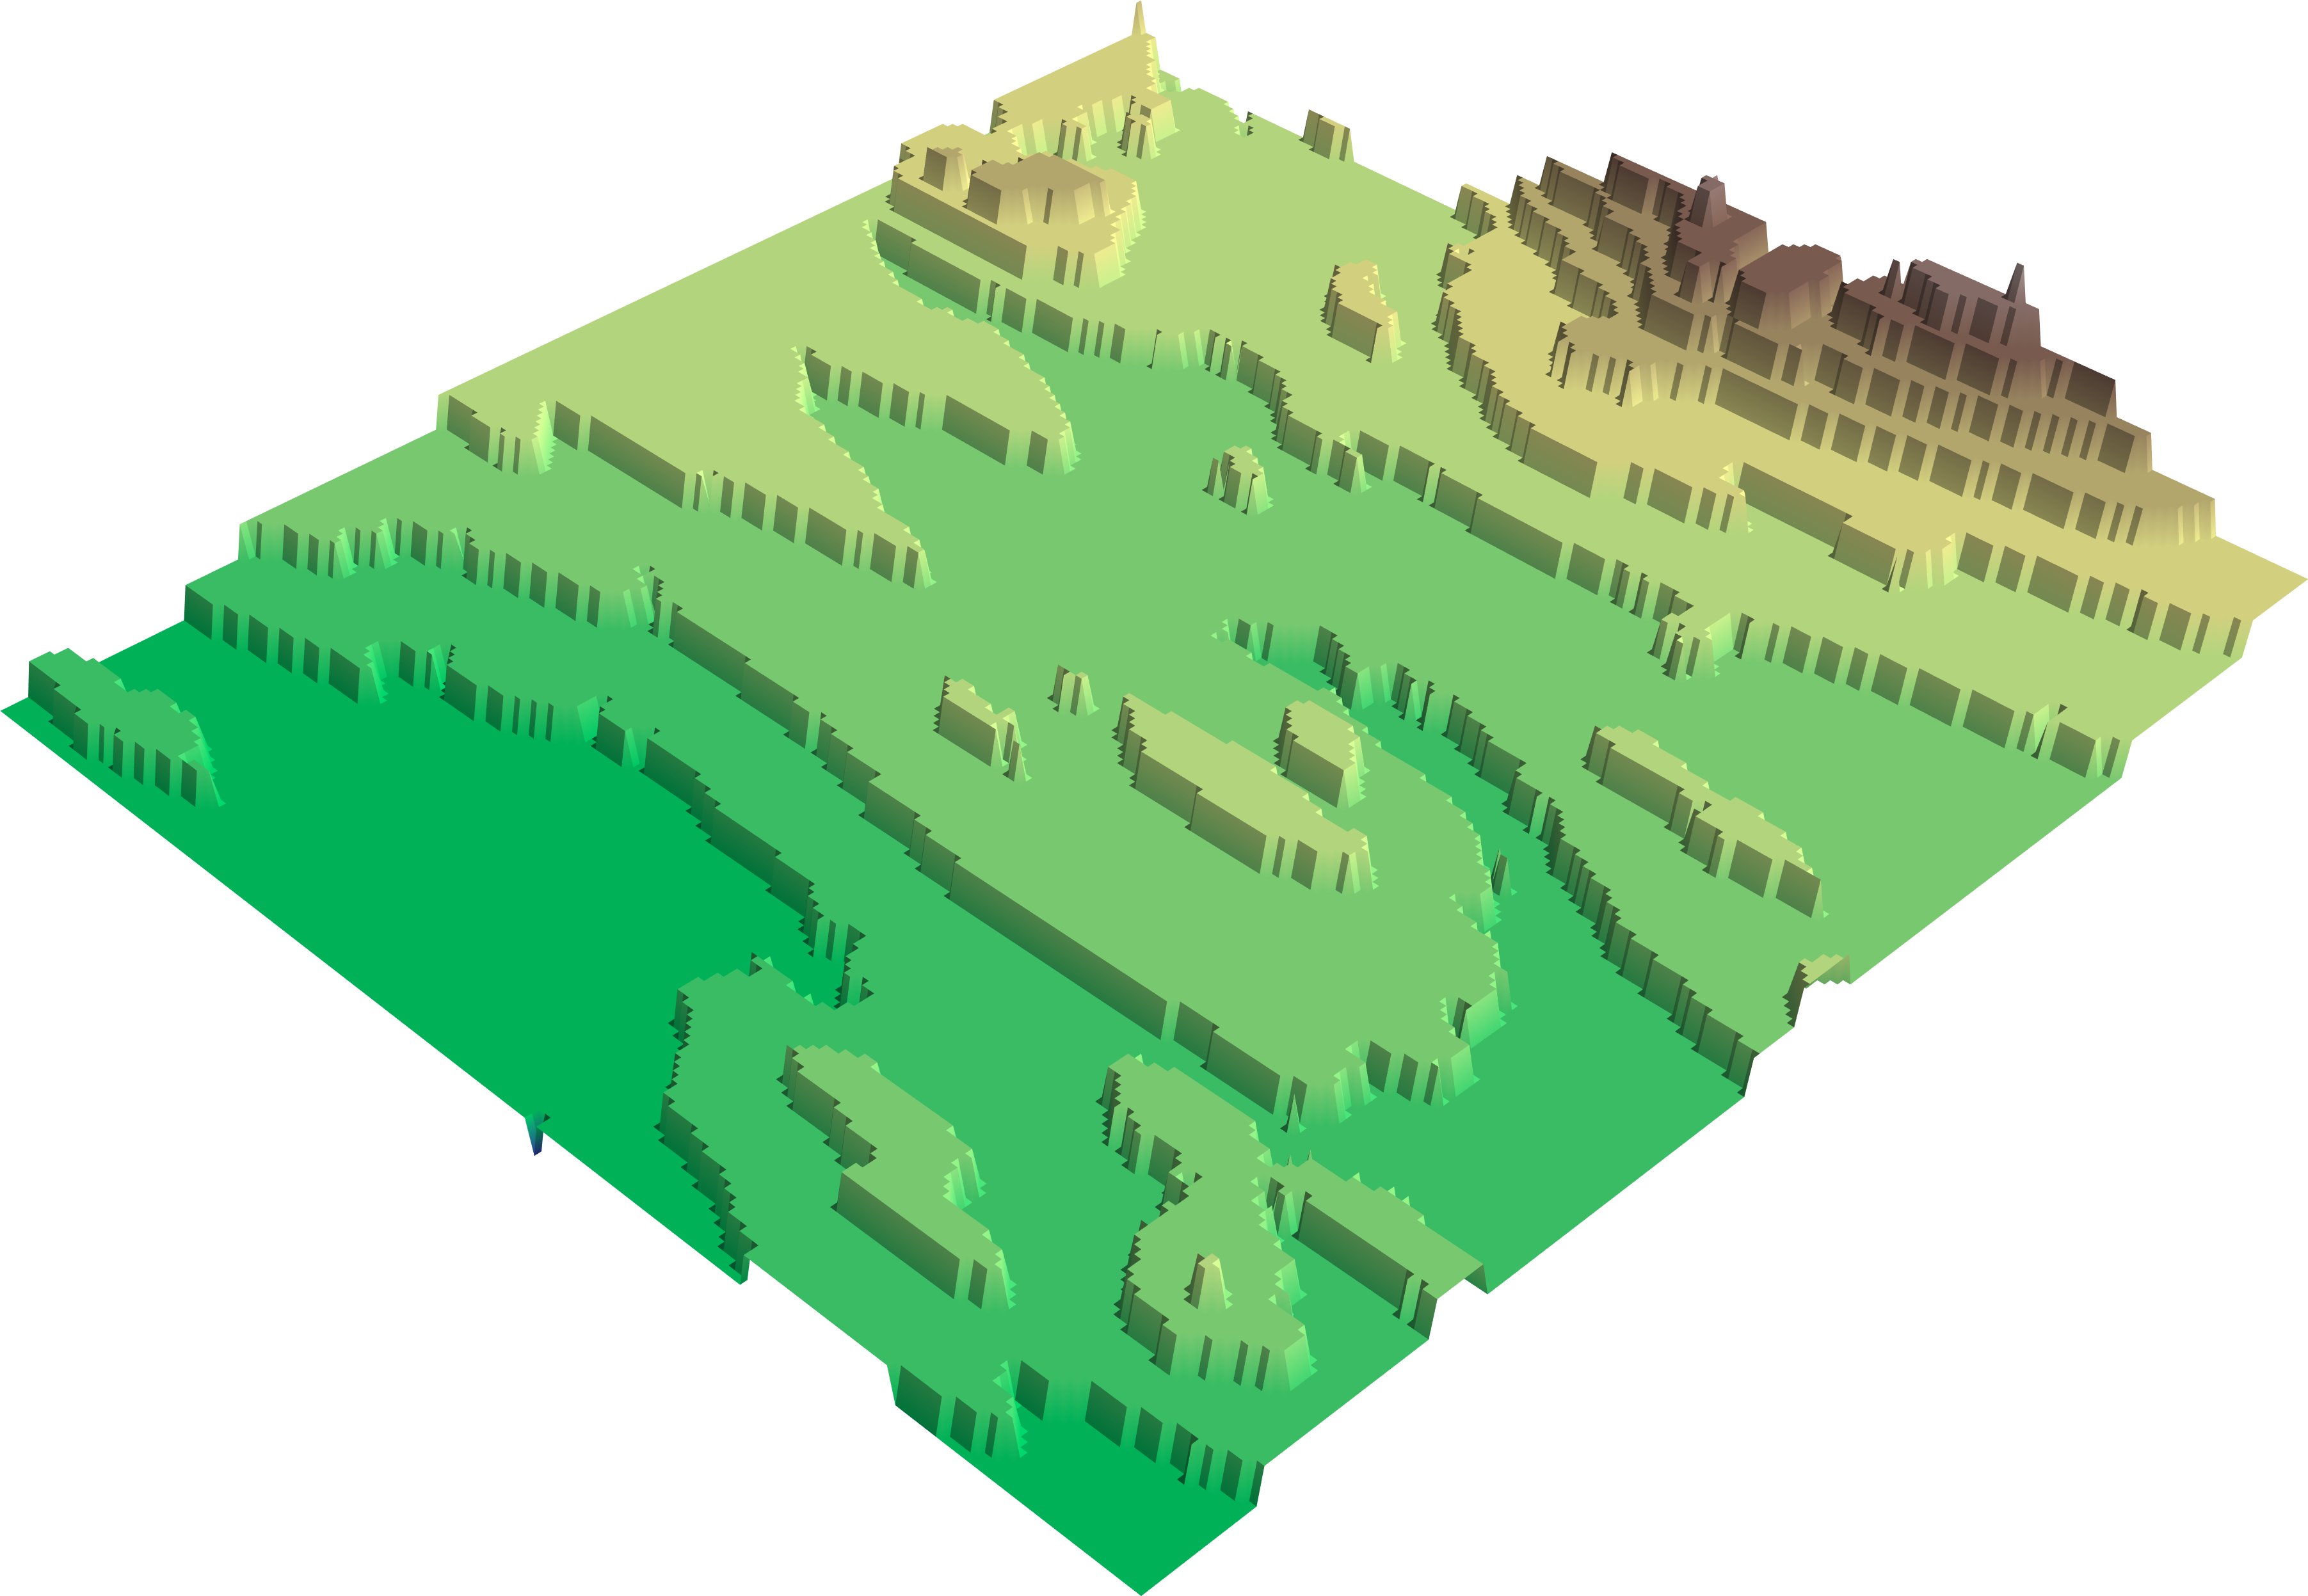
\includegraphics[width=\textwidth]{../images/NO33/2D_Data_Interpolation_3D_discretized_datagrid.png}
        \renewcommand\thesubfigure{\alph{subfigure}) i}
        \caption{Surface from discretized elevation data.}
        \end{subfigure}
        \hfill
        \begin{subfigure}{.49\textwidth}
            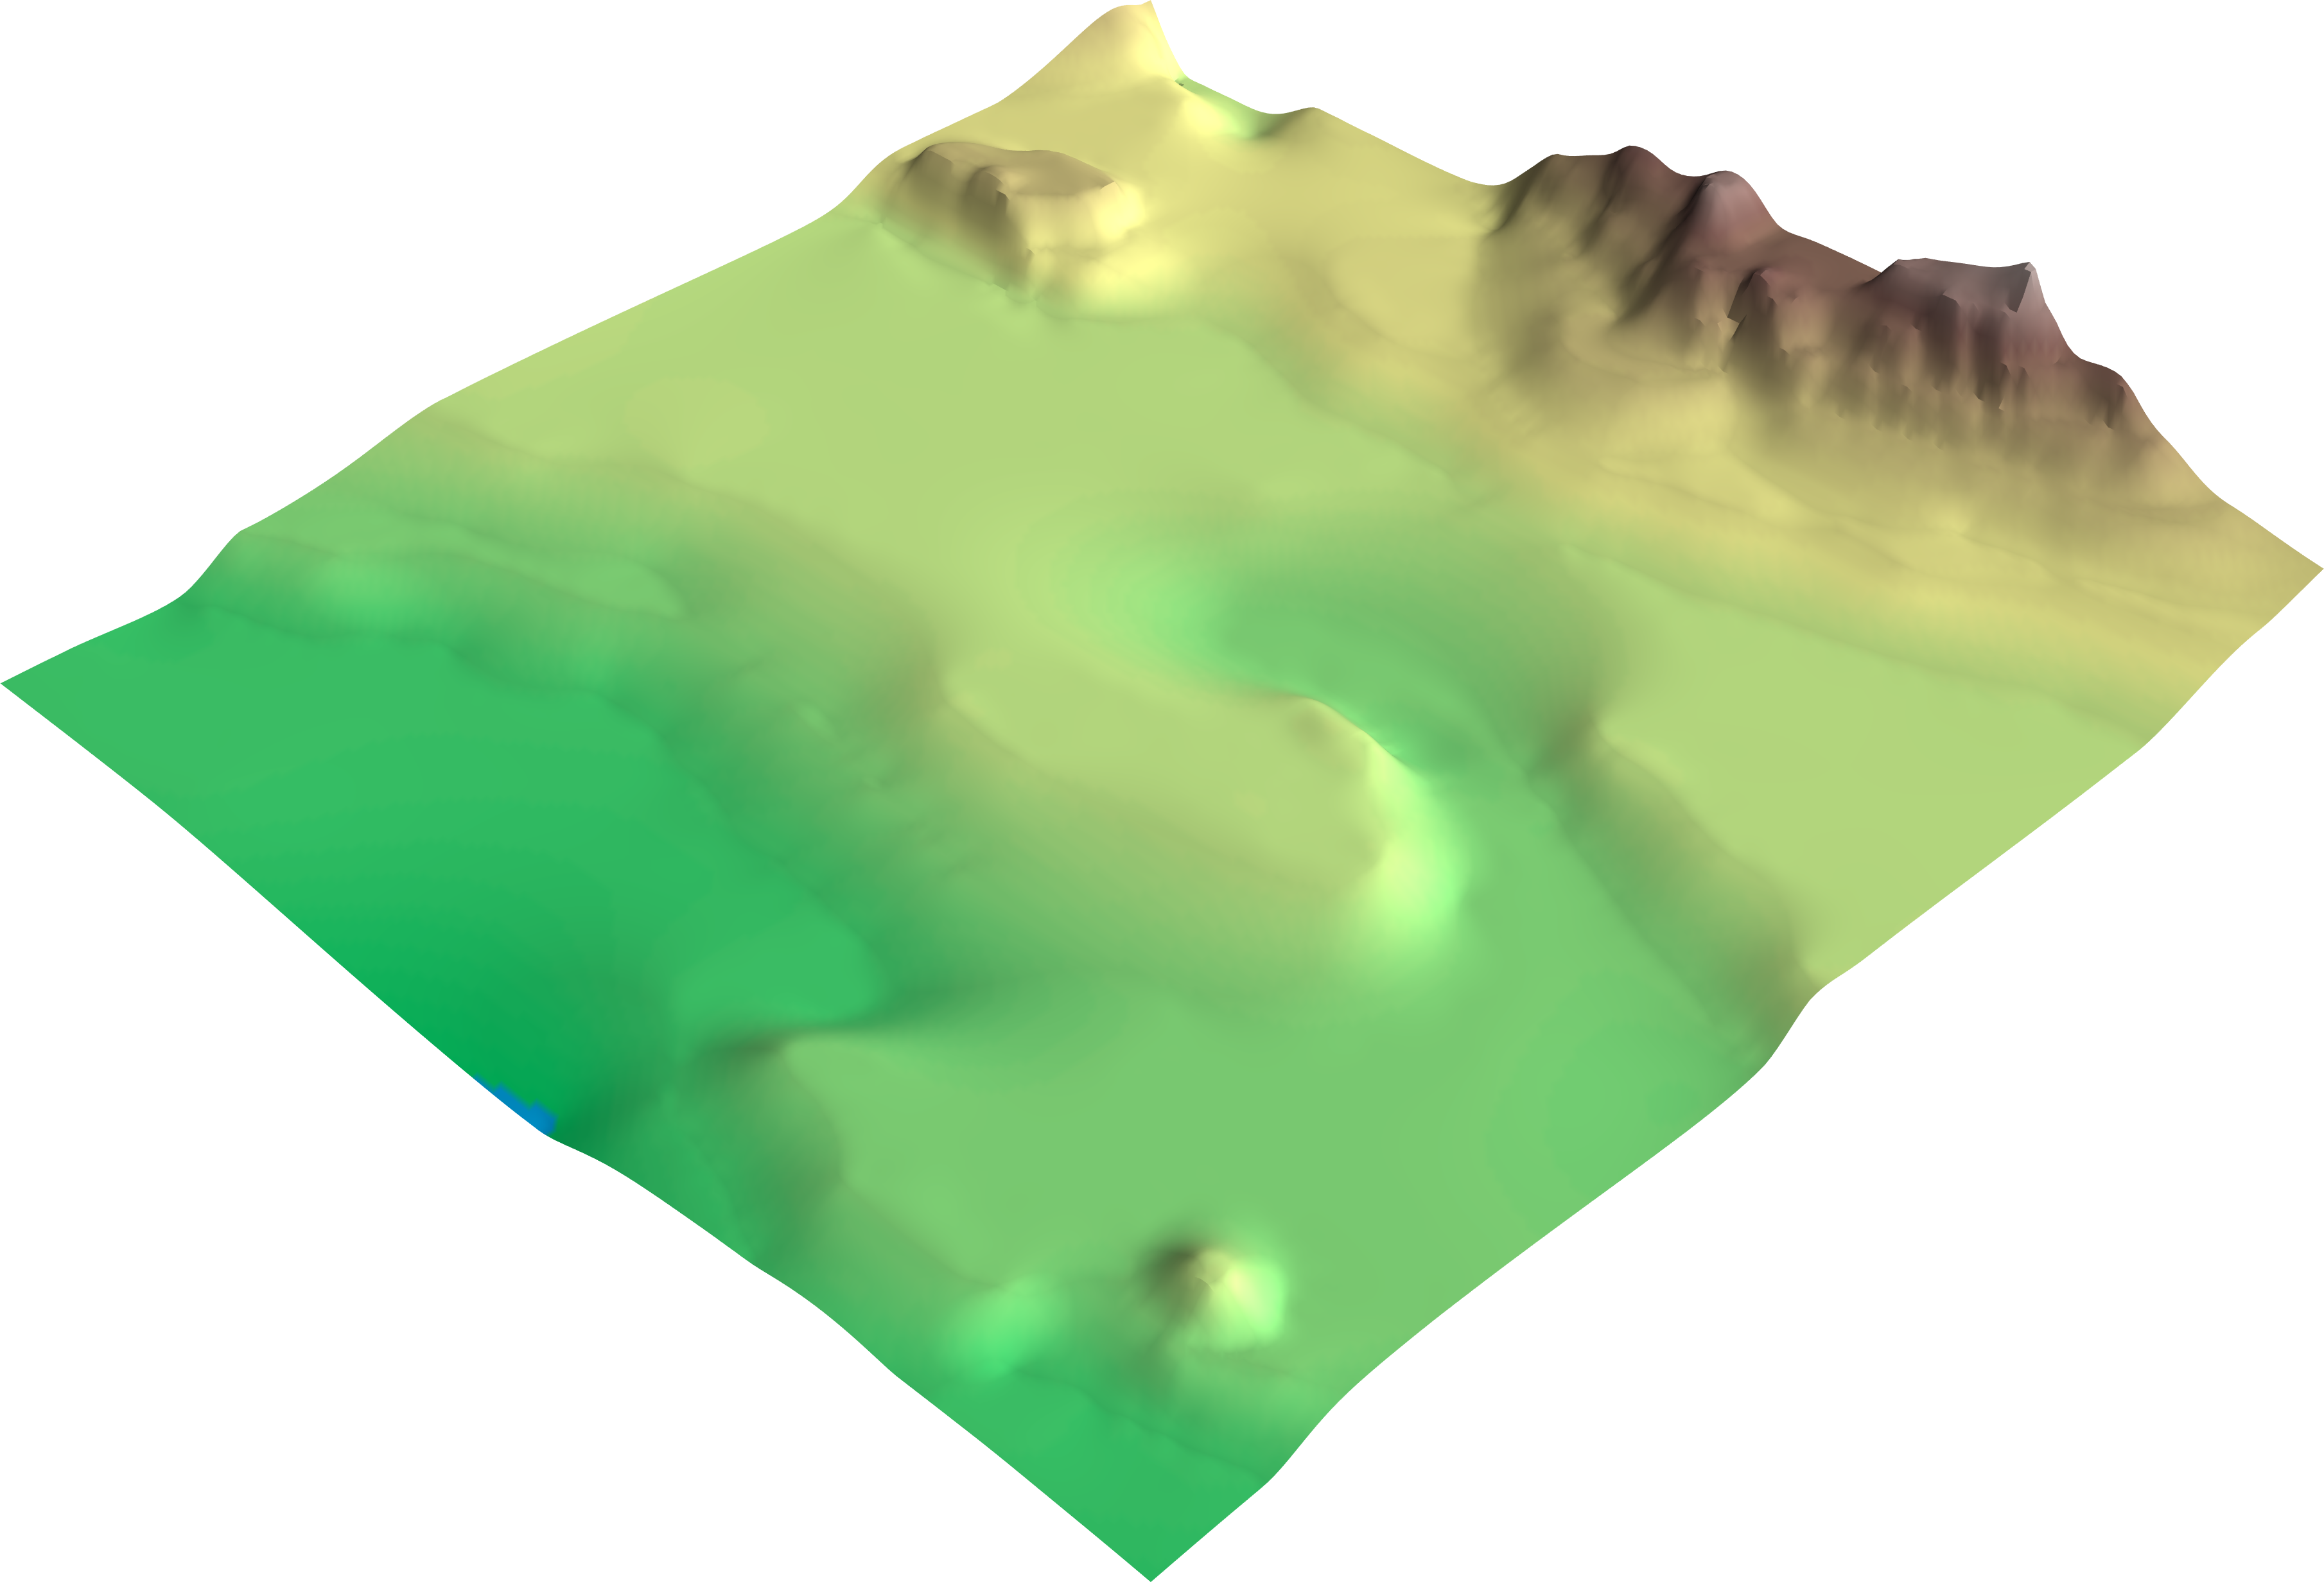
\includegraphics[width=\textwidth]{../images/NO33/2D_Data_Interpolation_3D_discretized_datagrid_interpolated.png}
        \addtocounter{subfigure}{-1}
        \renewcommand\thesubfigure{\alph{subfigure}) ii}
        \caption{Surface from interpolated elevation data.}
        \end{subfigure}
        \addtocounter{subfigure}{-1}
        \renewcommand\thesubfigure{\alph{subfigure}}
        \caption{Elevation data from west Dundee (UK ordnance tile NO33), southeast view.}
        \label{fig:3D_discretized_interpolation_b}
    \end{subfigure}
    \caption{Interpolating discretized elevation surface by using thin plate spline method.}
    \label{fig:3D_discretized_interpolation}
\end{figure}

\subsubsection{Limitations}
It's worth to mention that the interpolation approach for discretized elevation does not behave optimally at local maxima or local minima. This can be seen on Figure \ref{fig:3D_discretized_interpolation_a} in the top right part. A valley is lost in the interpolation process, due to the algorithm by which we select contour lines. The outline of the valley is conserved for the interpolation with elevation value of the higher plateau ($200$ $m$), whilst no further information is preserved about the valley. If interpolation of higher accuracy is desired for DEMs, a revised algorithm should be implemented.

\chapter{Interpolating Binary Contours in 3D}\label{chap:3D}

Interpolating binary contours is useful in case when a contour is produced by applying marching squares to binary data. This is usually done in order to create a triangular mesh, so that a smooth surface from the boundary of the binary data is produced. Rendering a mesh is also computationally cheaper then rendering the voxels individually. However, the resulting contour looks in this case still looks very voxelated. In this chapter, we'll investigate several methods how the smoothness of produced binary contours can be improved.
\begin{figure}[H]
    \centering
    \begin{subfigure}{.49\textwidth}
        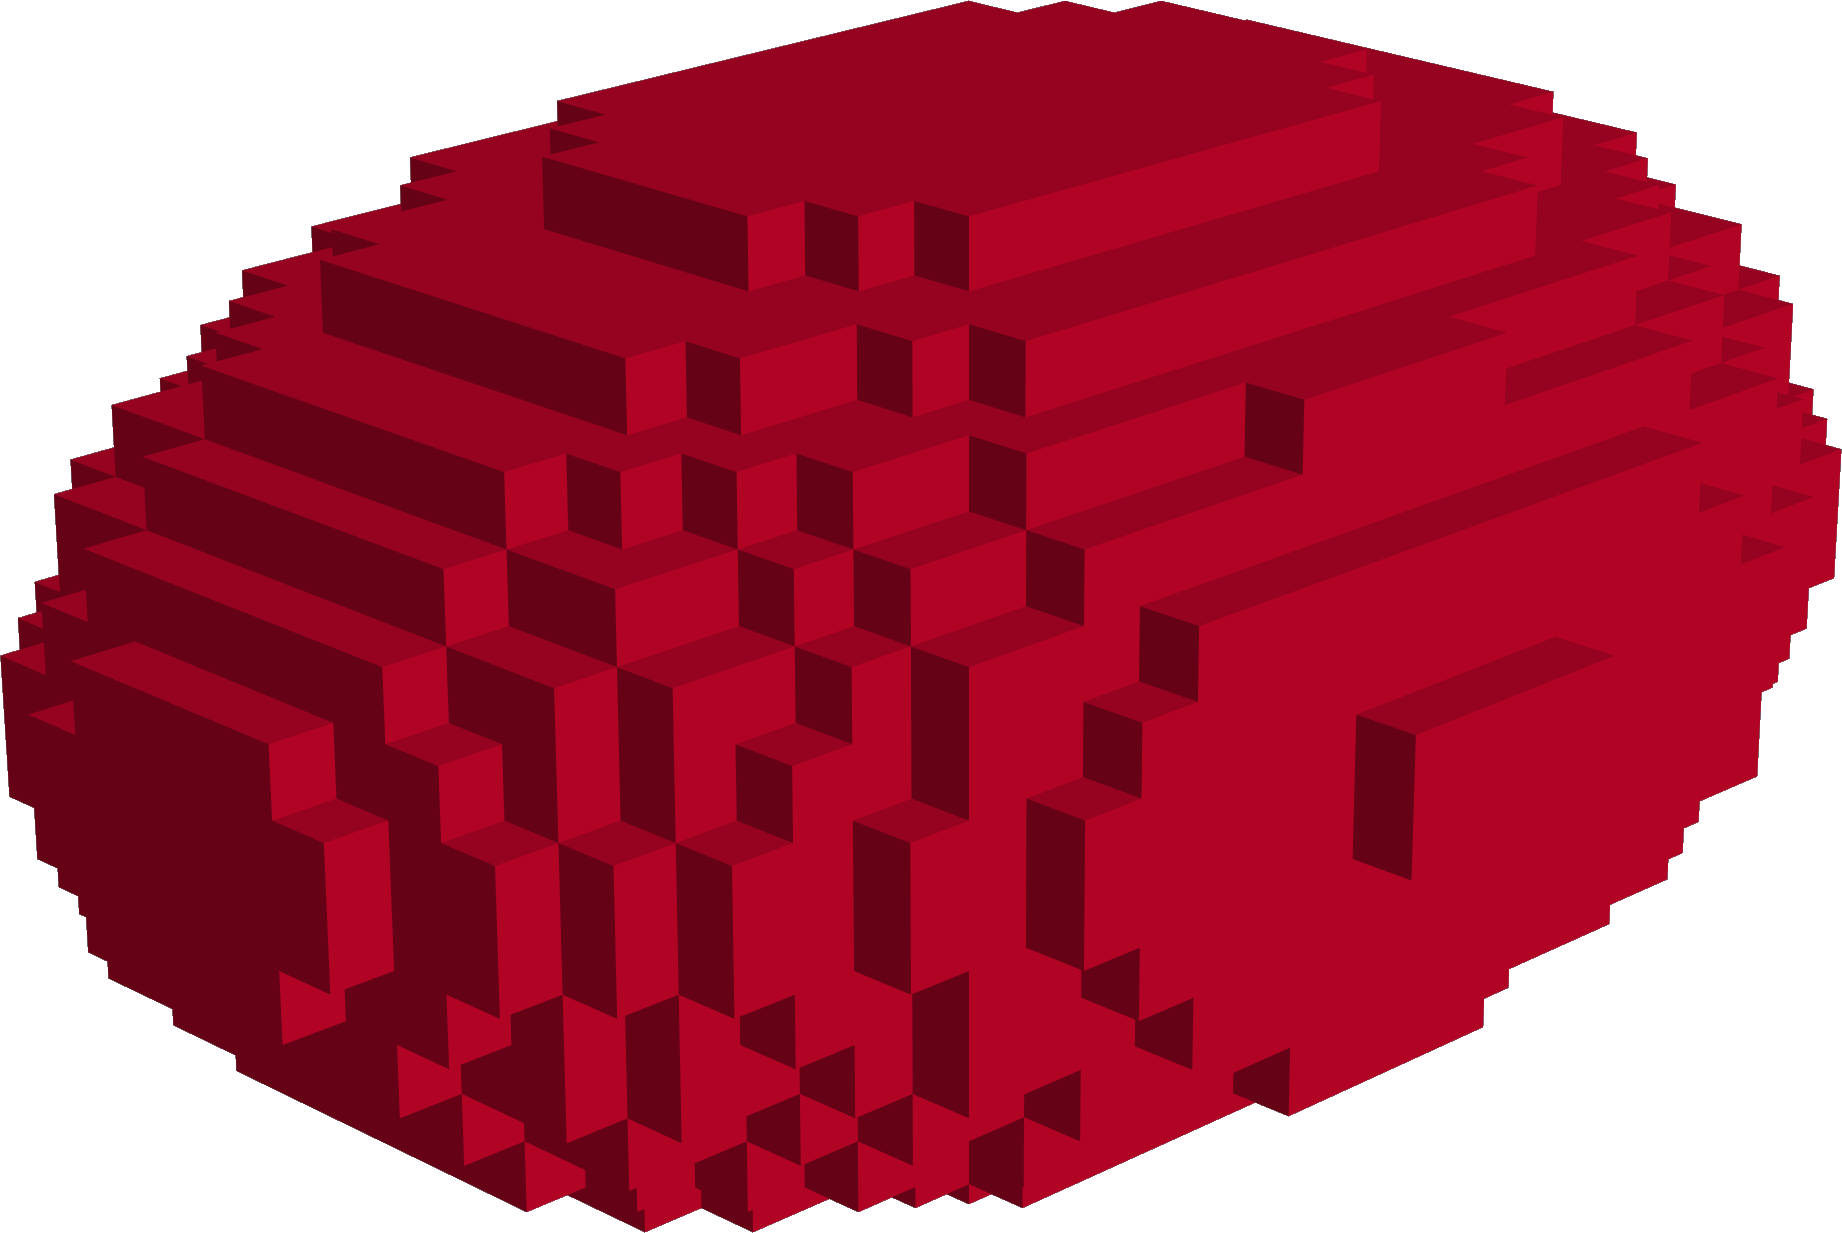
\includegraphics[width=\textwidth]{../images/3D/Ellipsoid_blocks.png}
    \caption{The data voxels rendered directly.}
    \label{fig:Ellipsoid_blocks}
    \end{subfigure}
    \hfill
    \begin{subfigure}{.49\textwidth}
        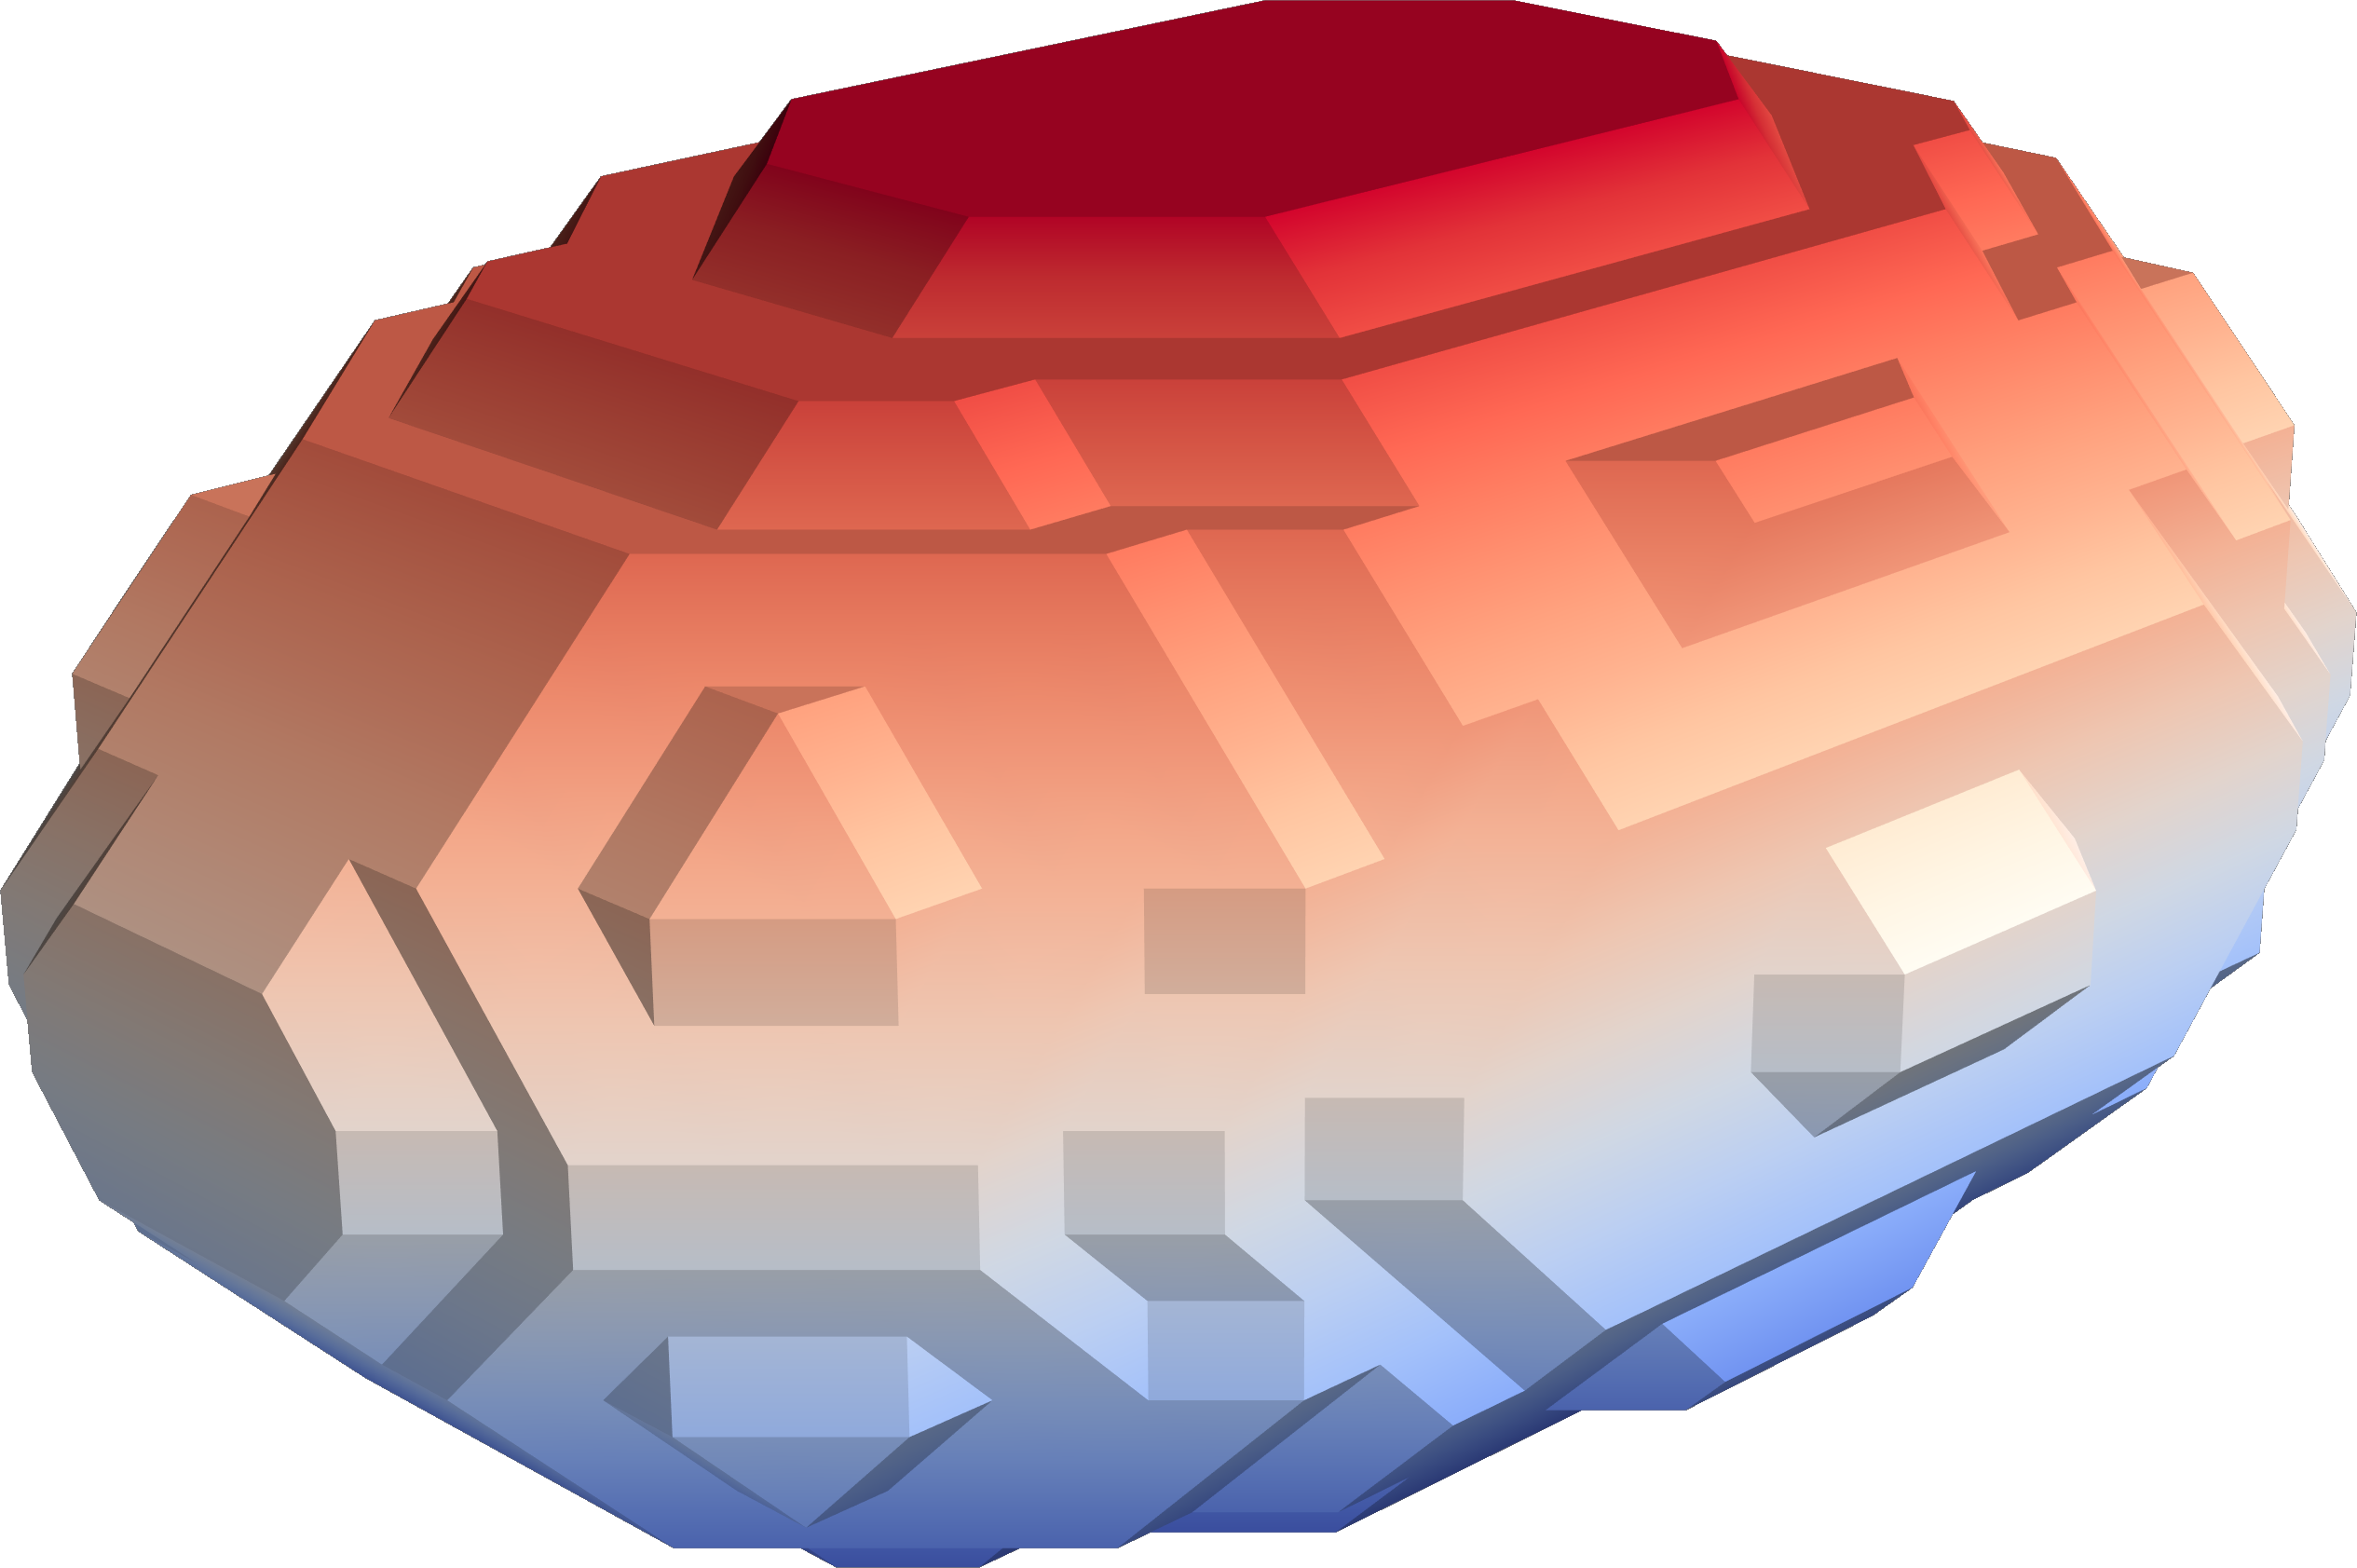
\includegraphics[width=\textwidth]{../images/3D/Ellipsoid_marching_squares.png}
    \caption{The triangular mesh produced by marching squares.}
    \label{fig:Ellipsoid_marching_squares}
    \end{subfigure}
    \caption{Comparison between rendering voxels of an ellipsoid directly and applying marching squares algorithm.}
    \label{fig:Ellipsoid}
\end{figure}

\section{Block Averaging}\label{sec:block_avg}

Block averaging is a relatively simple method to smoothen the binary data. Only regions on the boundary of the contour are changed by using this method, and no distortion in shape is caused. Block averaging is also easy to implement, as it requires no more than a for loop, or a convolution function with uniform kernel.
\begin{figure}[H]
    \centering
    \begin{subfigure}{.49\textwidth}
        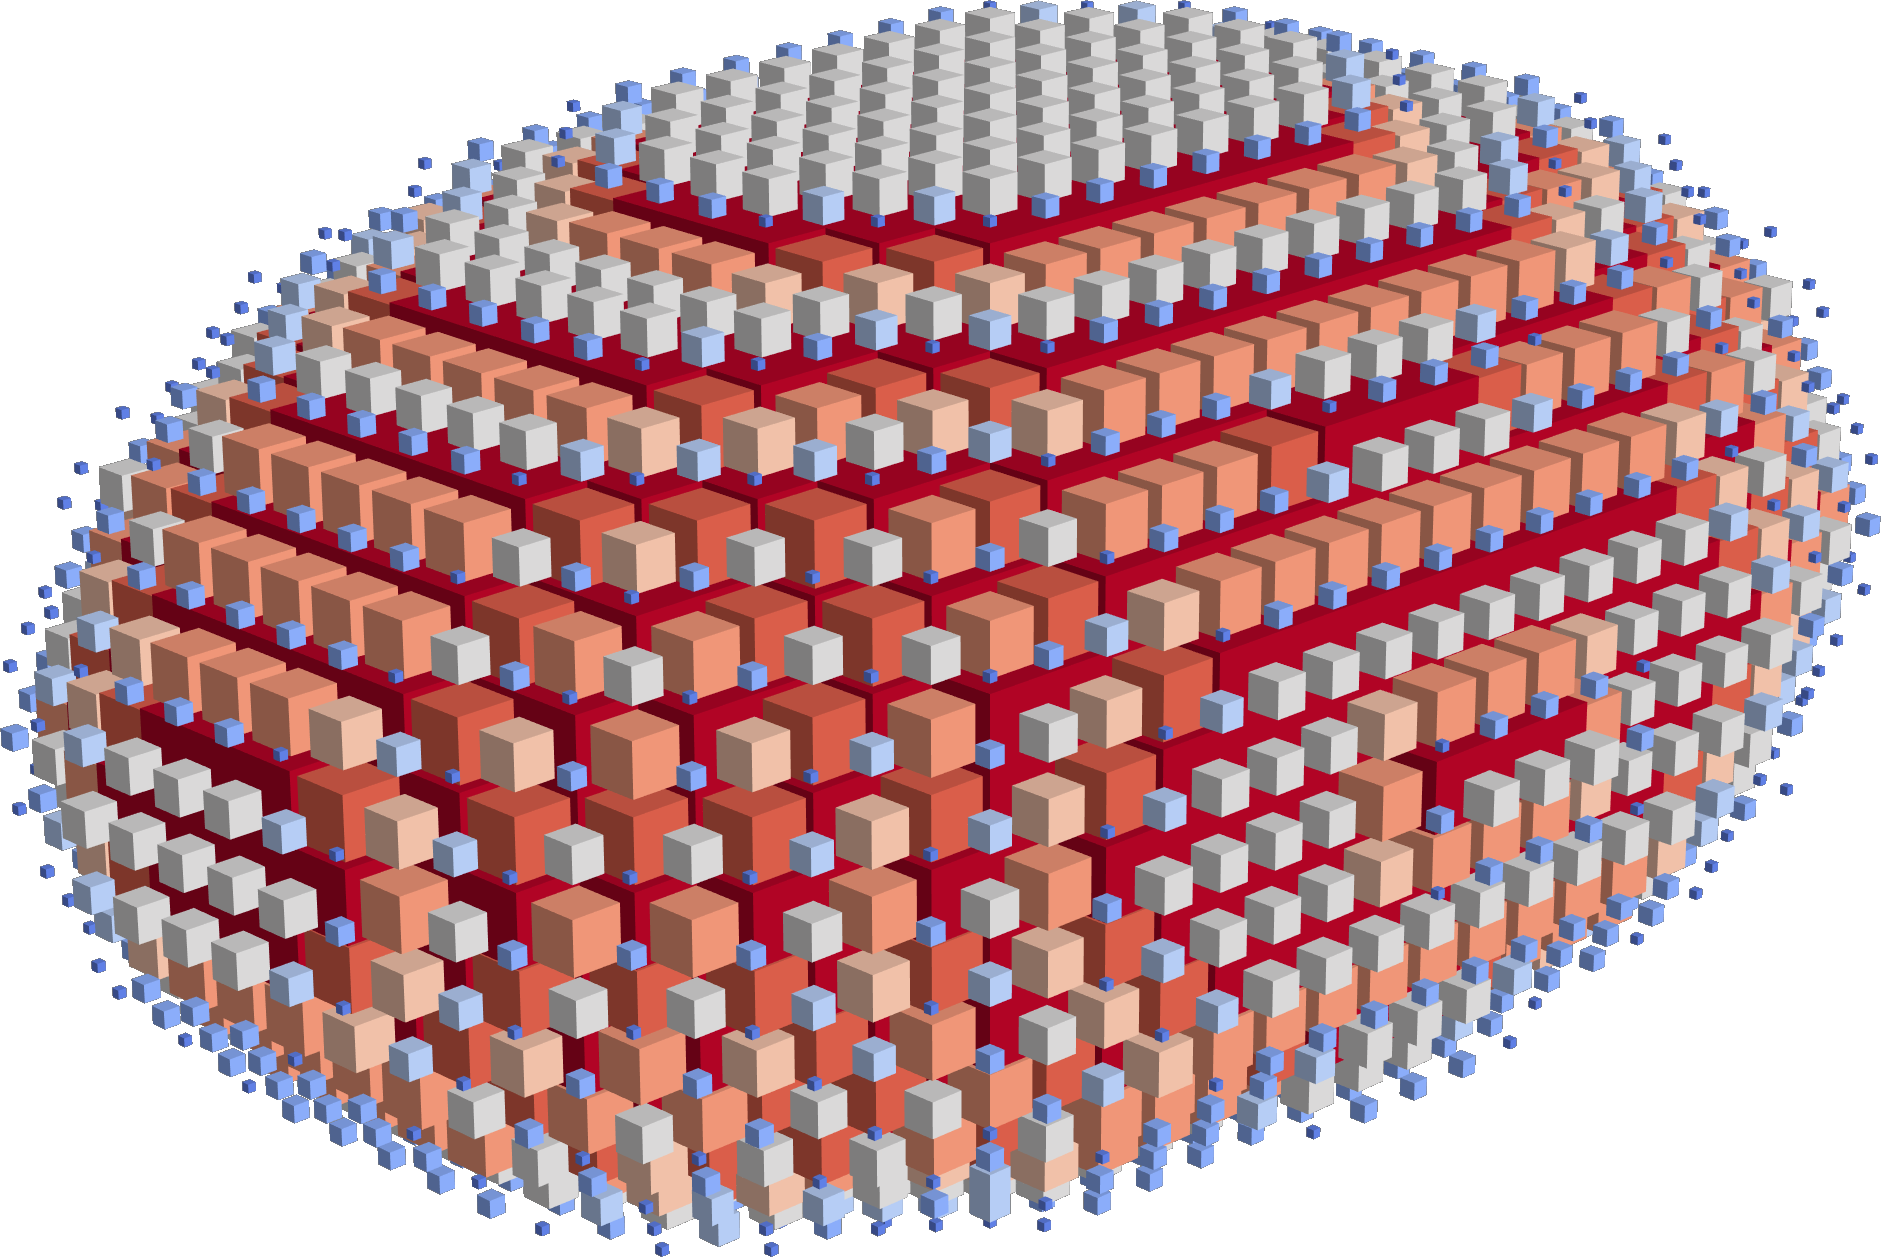
\includegraphics[width=\textwidth]{../images/3D/Ellipsoid_blocks_block_avg.png}
    \caption{The data voxels rendered directly.}
    \label{fig:Ellipsoid_blocks_block_avg}
    \end{subfigure}
    \hfill
    \begin{subfigure}{.49\textwidth}
        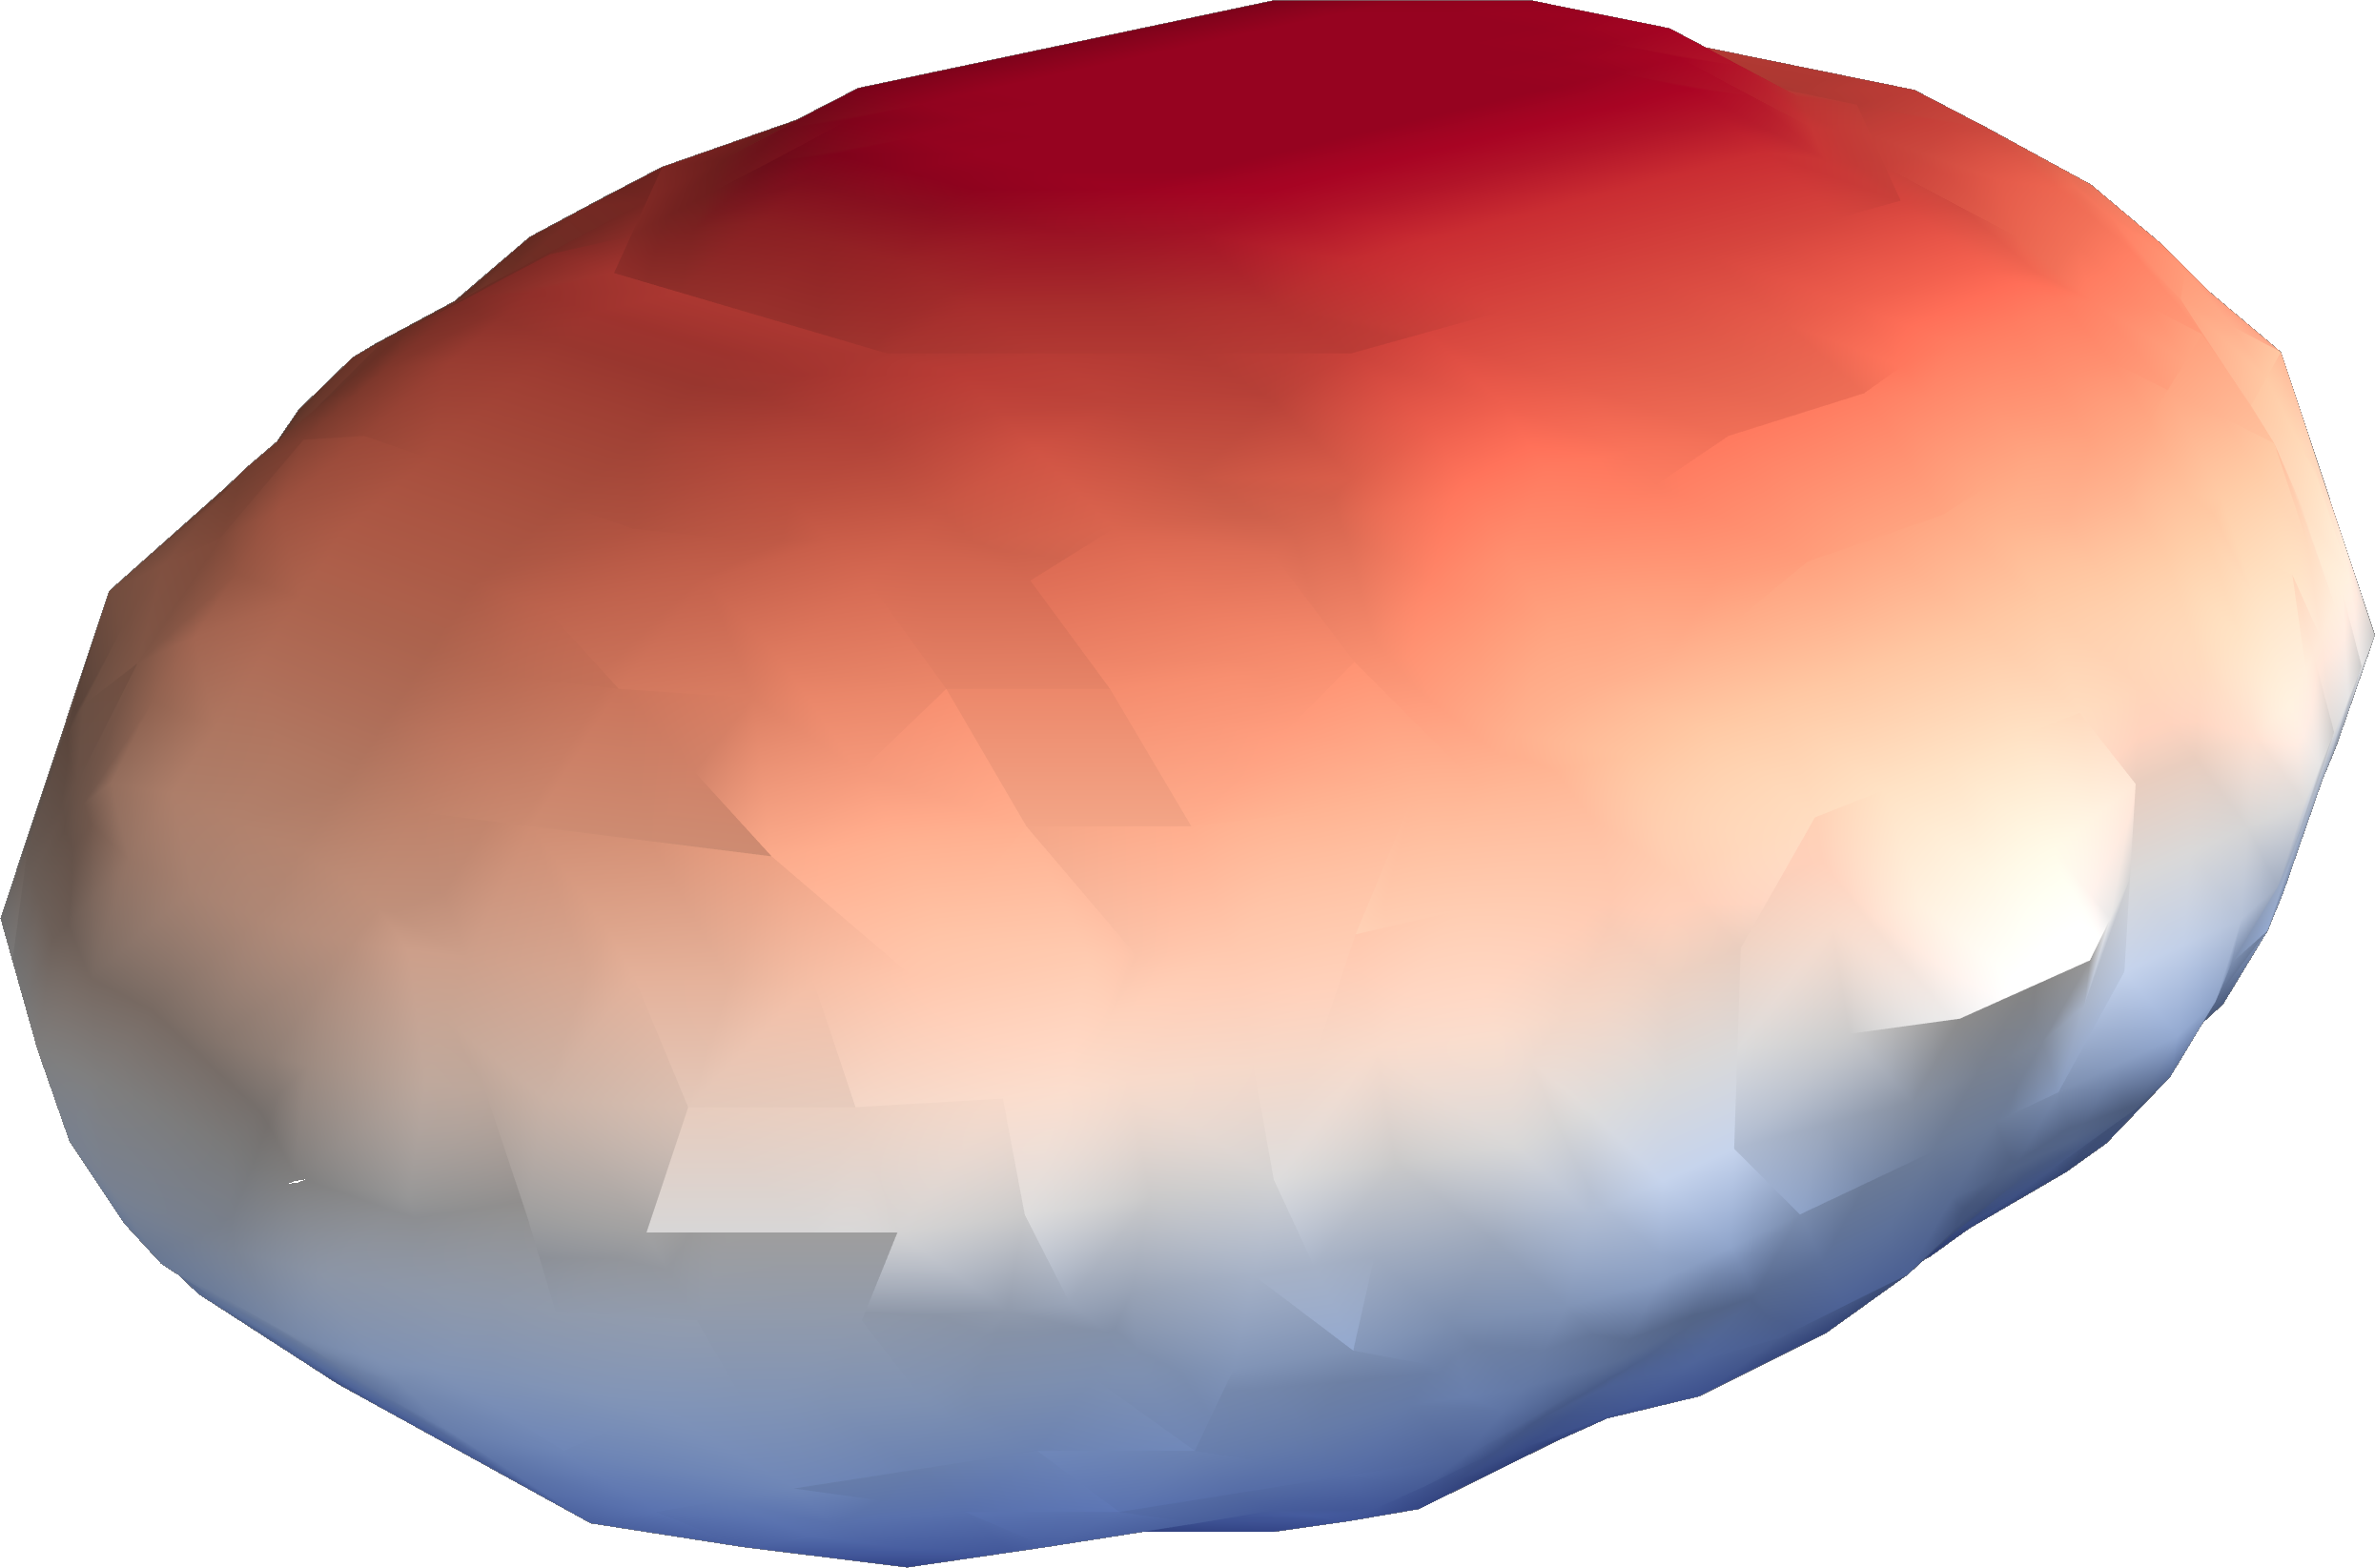
\includegraphics[width=\textwidth]{../images/3D/Ellipsoid_marching_squares_block_avg.png}
    \caption{The triangular mesh produced by marching squares.}
    \label{fig:Ellipsoid_marching_squares_block_avg}
    \end{subfigure}
    \caption{Comparison between rendering voxels directly and applying marching squares algorithm, after block averaging an ellipsoid with block size 2.}
    \label{fig:Ellipsoid_block_avg}
\end{figure}
\begin{figure}[H]
    \centering
    \begin{subfigure}{.49\textwidth}
        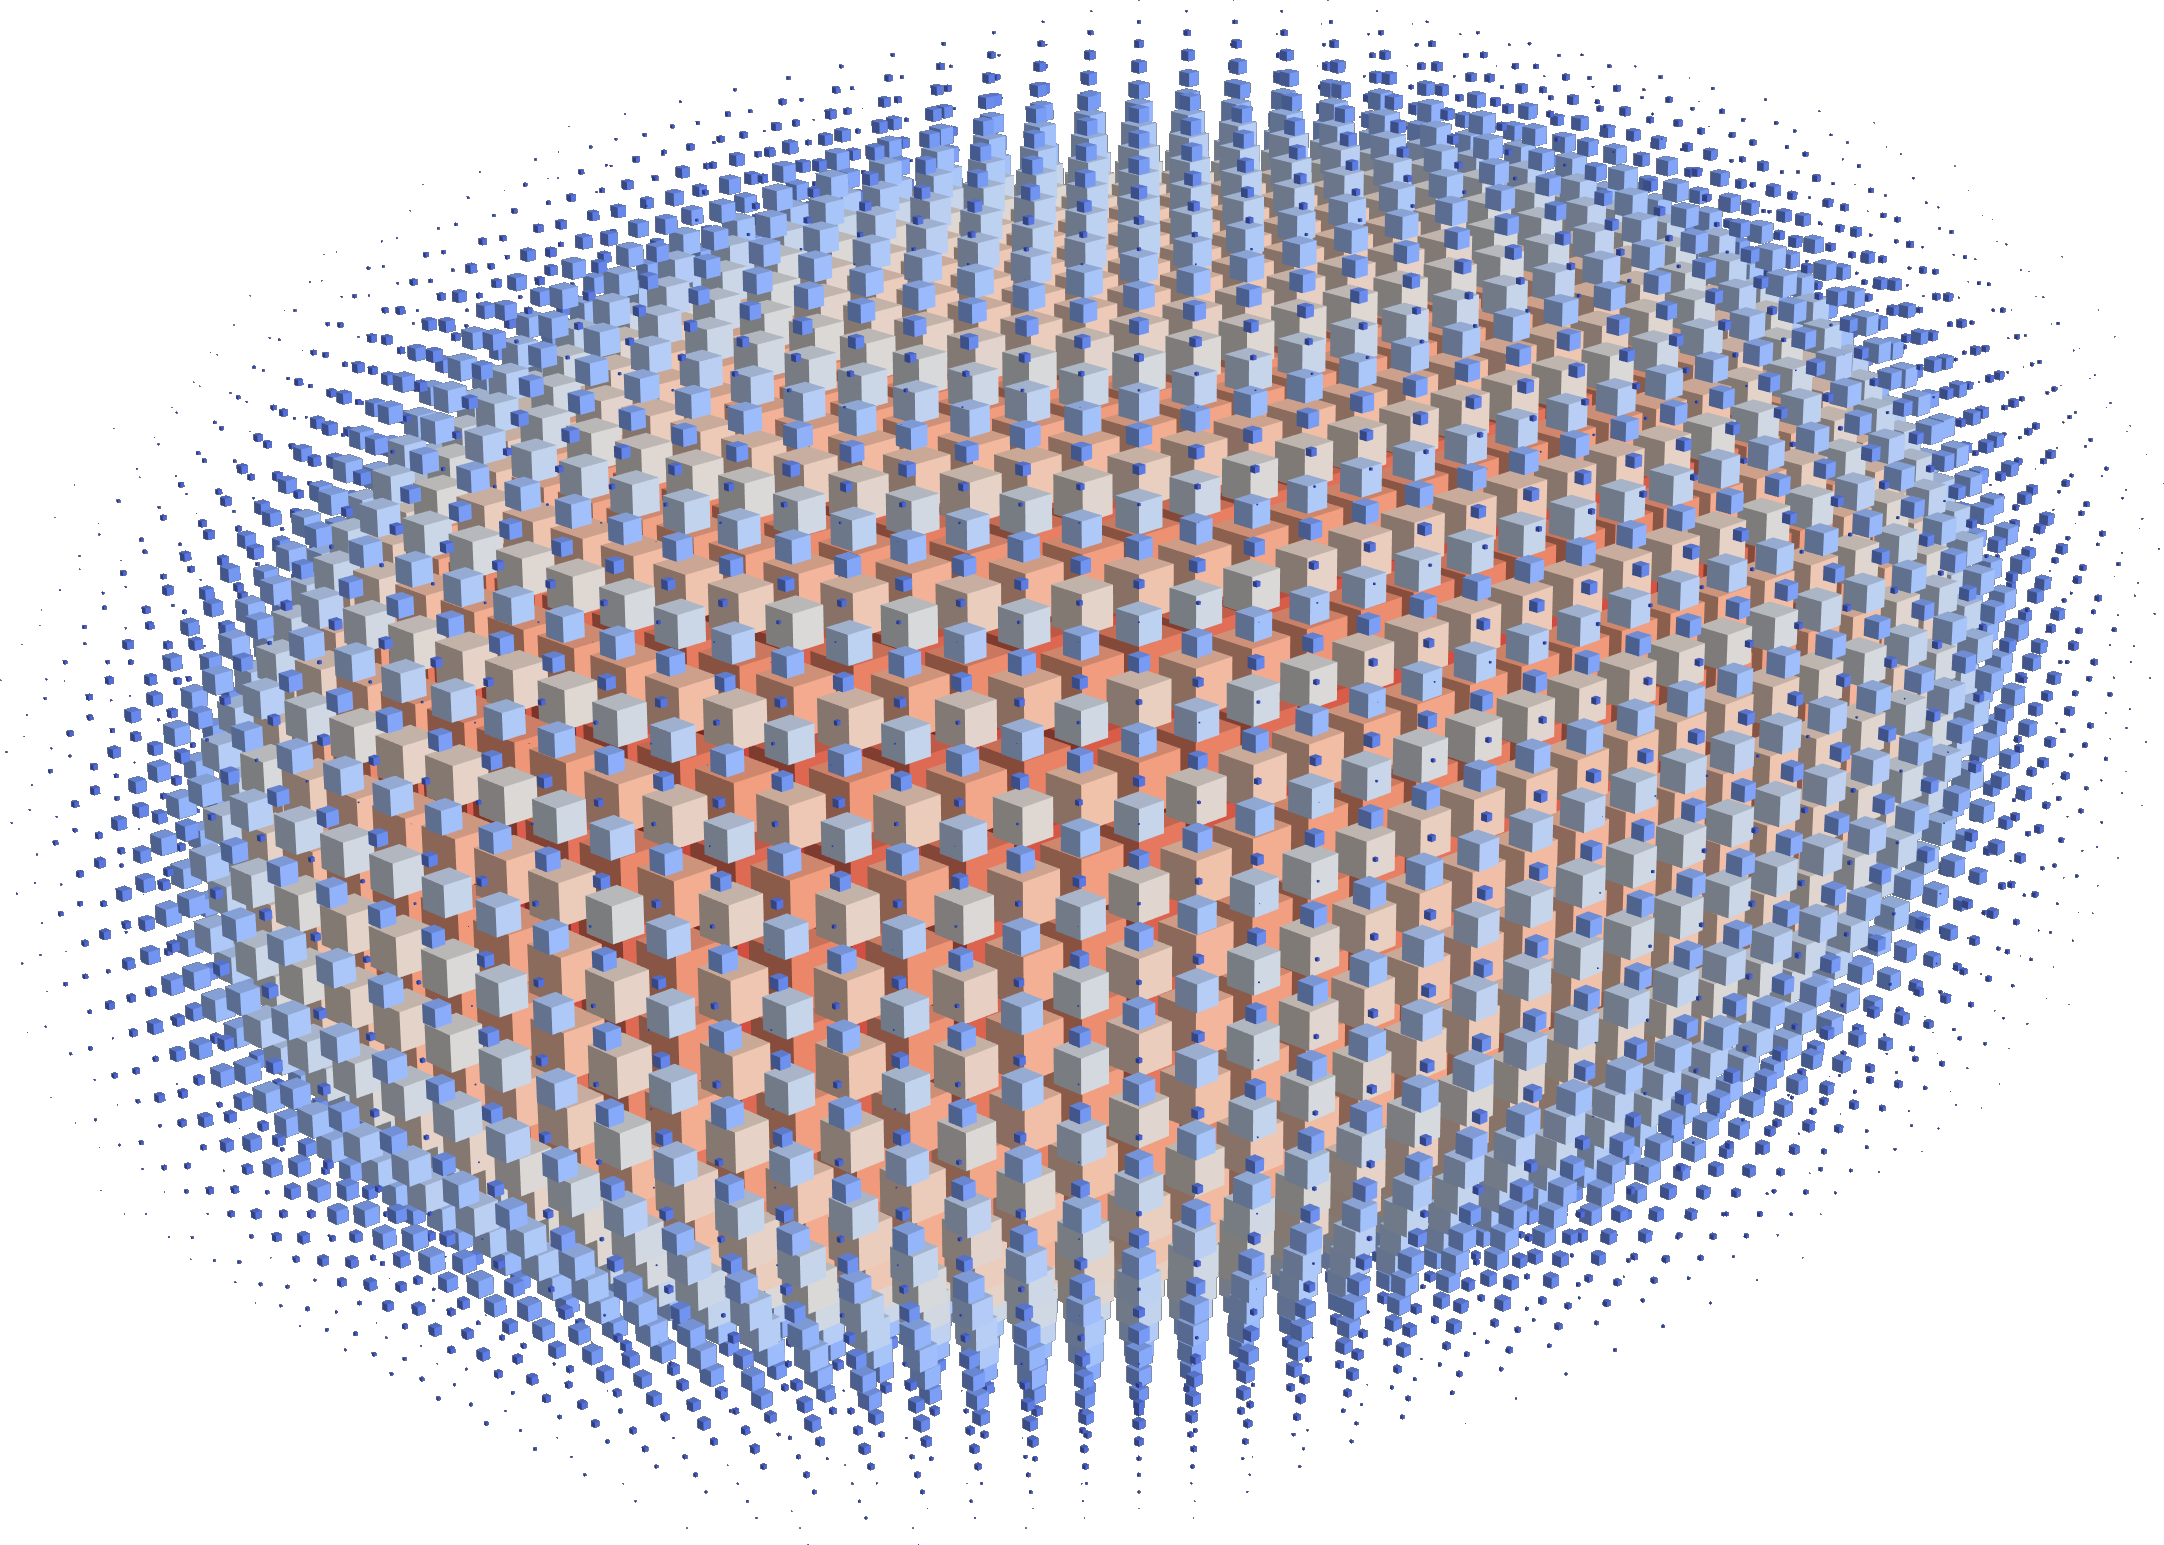
\includegraphics[width=\textwidth]{../images/3D/Ellipsoid_blocks_block_avg_5.png}
    \caption{The data voxels rendered directly.}
    \label{fig:Ellipsoid_blocks_block_avg_5}
    \end{subfigure}
    \hfill
    \begin{subfigure}{.49\textwidth}
        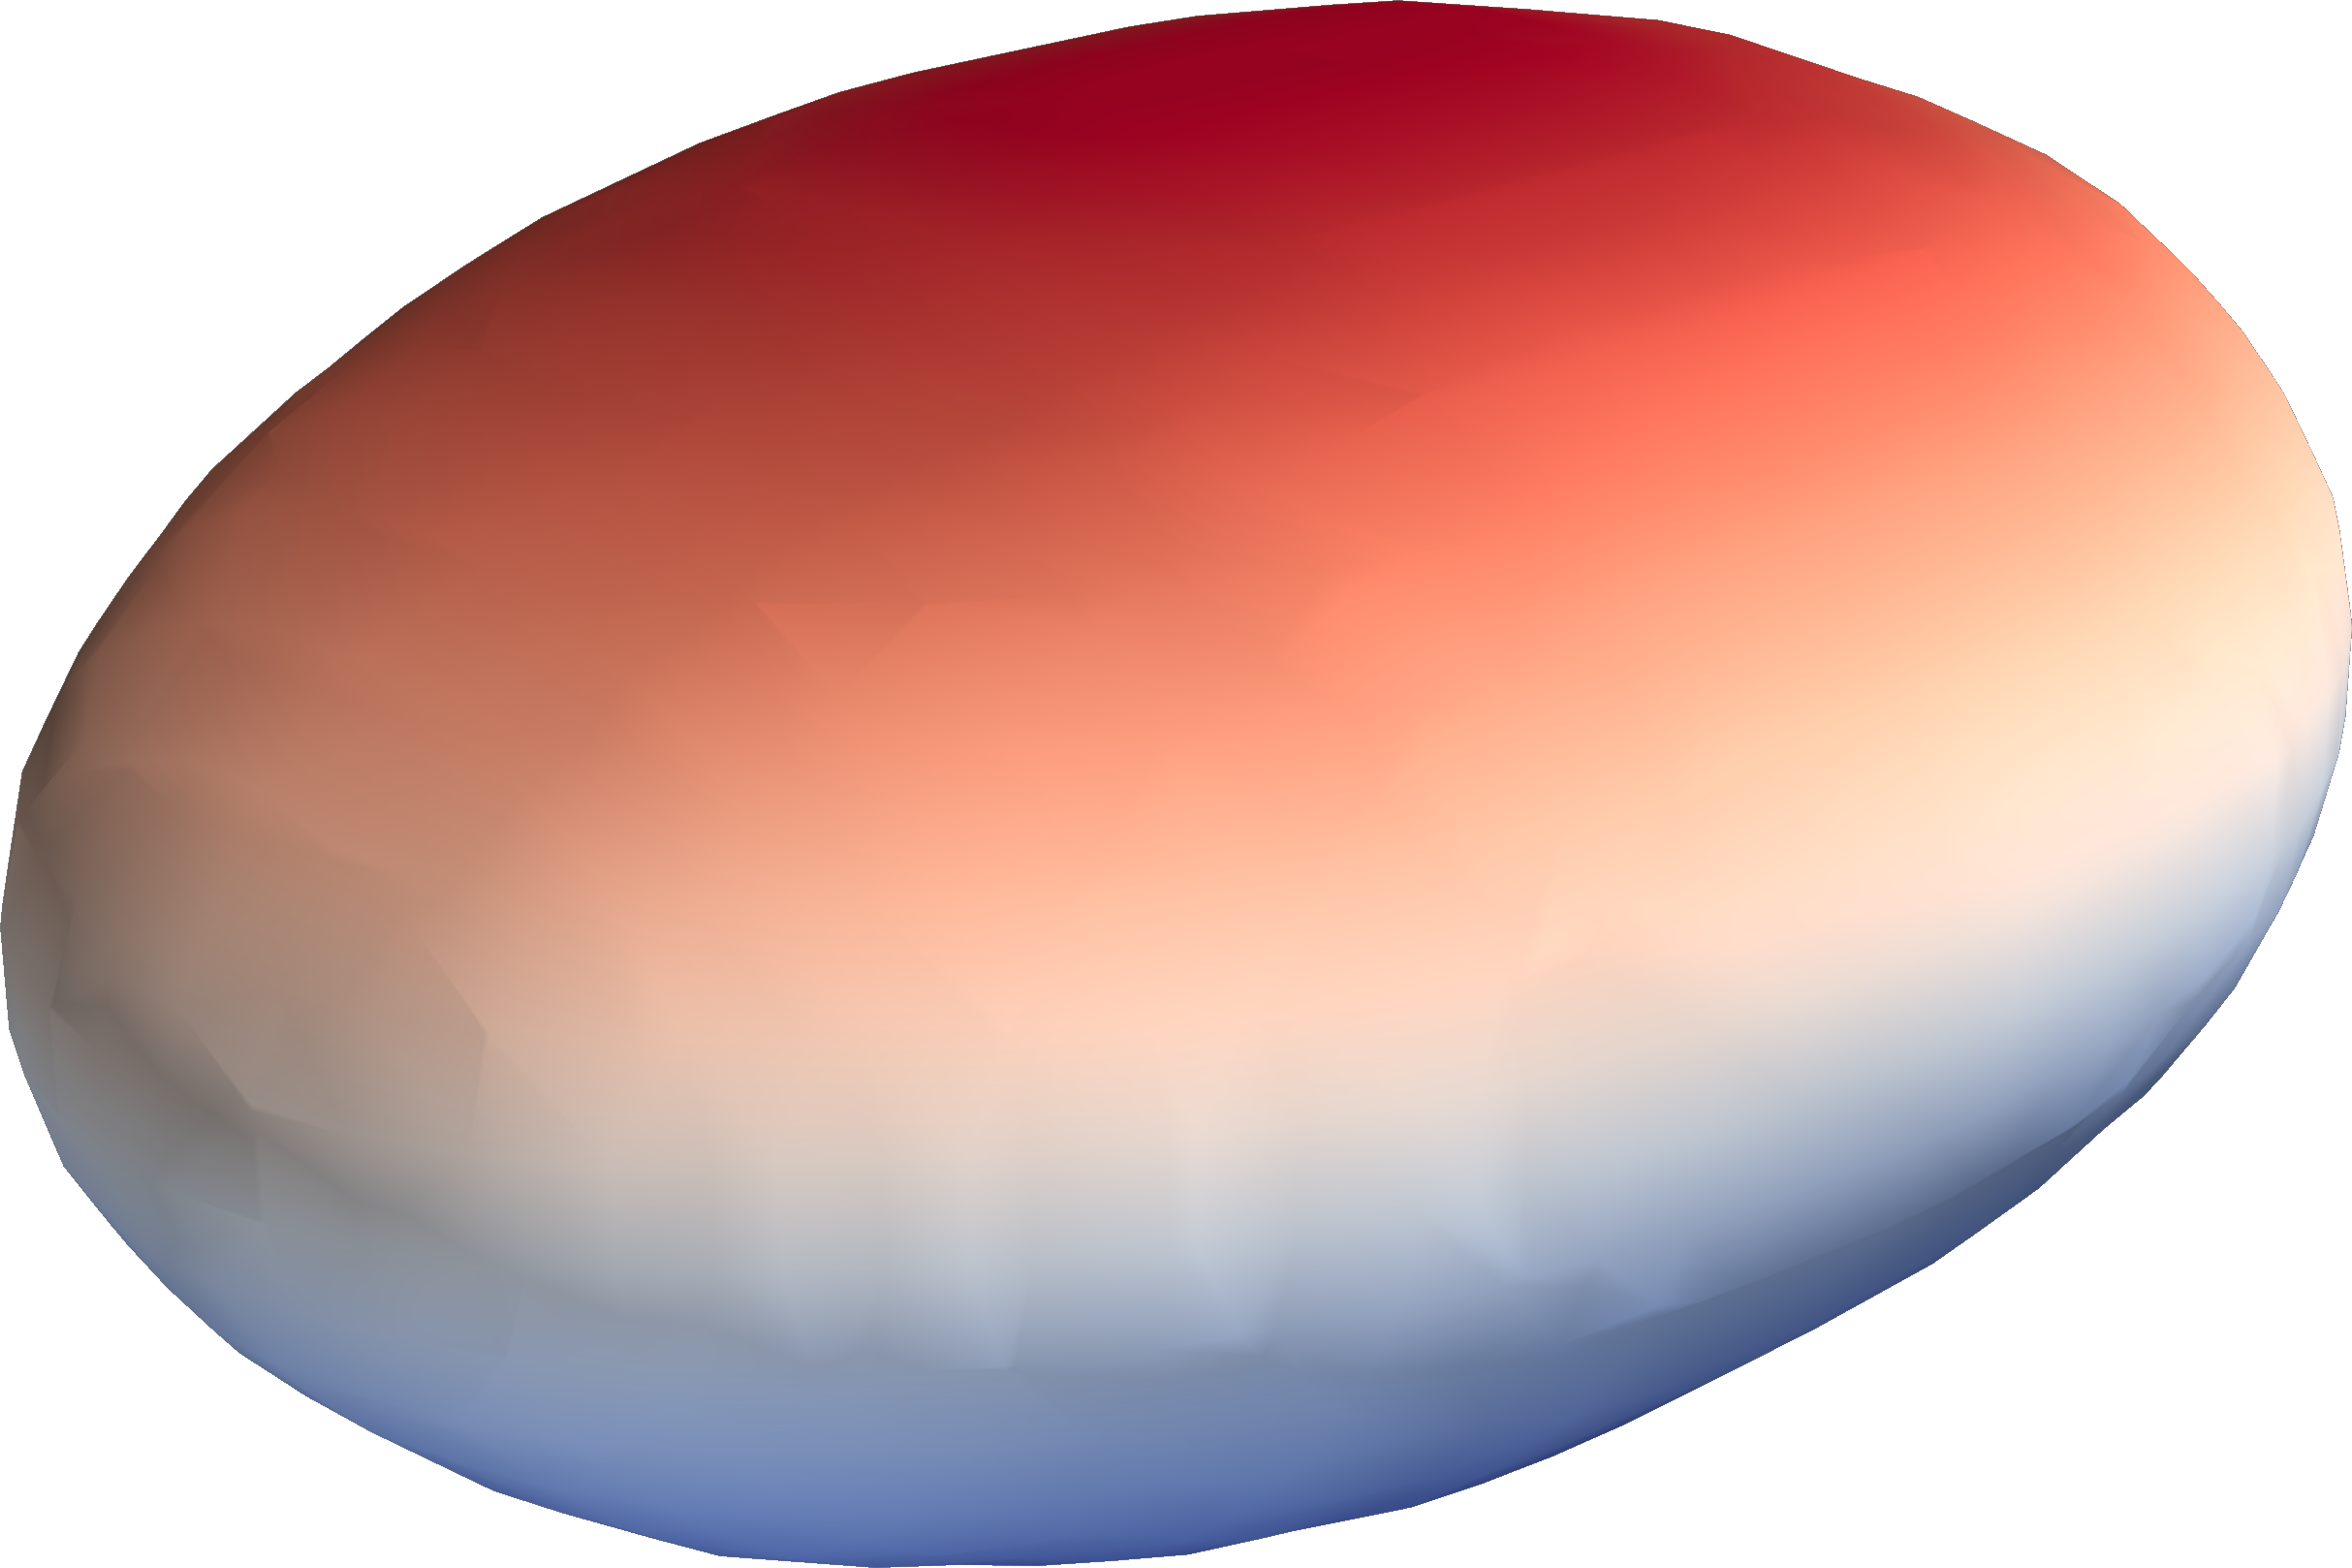
\includegraphics[width=\textwidth]{../images/3D/Ellipsoid_marching_squares_block_avg_5.png}
    \caption{The triangular mesh produced by marching squares.}
    \label{fig:Ellipsoid_marching_squares_block_avg_5}
    \end{subfigure}
    \caption{Comparison between rendering voxels directly and applying marching squares algorithm, after block averaging an ellipsoid with block size 5.}
    \label{fig:Ellipsoid_block_avg_5}
\end{figure}

\section{Isolation of corner vertices}
As an alternative to block averaging, we can identify a neighbourhood of the border and interpolate the points inside this region, as we know that on one side of the region the values are all $0$ and on the other they are all $1$. To identify this region, we can isolate the corner vertices from the binary data. These vertices can be identified by looking at block sums. If a sum of a $n\times n \times n$ block is $1$, then we can consider this block as the \textit{external} corner and if it is $n^3-1$, then we can consider the block to be the \textit{internal} corner. And finally, if the sum is not $0$ or $n^3$, we mark the points of this block as \textit{boundary} points.

After isolating the corners, we can apply various interpolation techniques to interpolate all the points in the \textit{boundary} region by using the corner vertices as value sources. An example that works quite well is using Delaunay tetrahedral tesselation and subsequent linear barycentric interpolation. The tesselation is created from the corner vertices and all boundary vertices' values are interpolated linearly from this tesselation.

\begin{figure}[H]
    \centering
    \begin{subfigure}{.32\textwidth}
        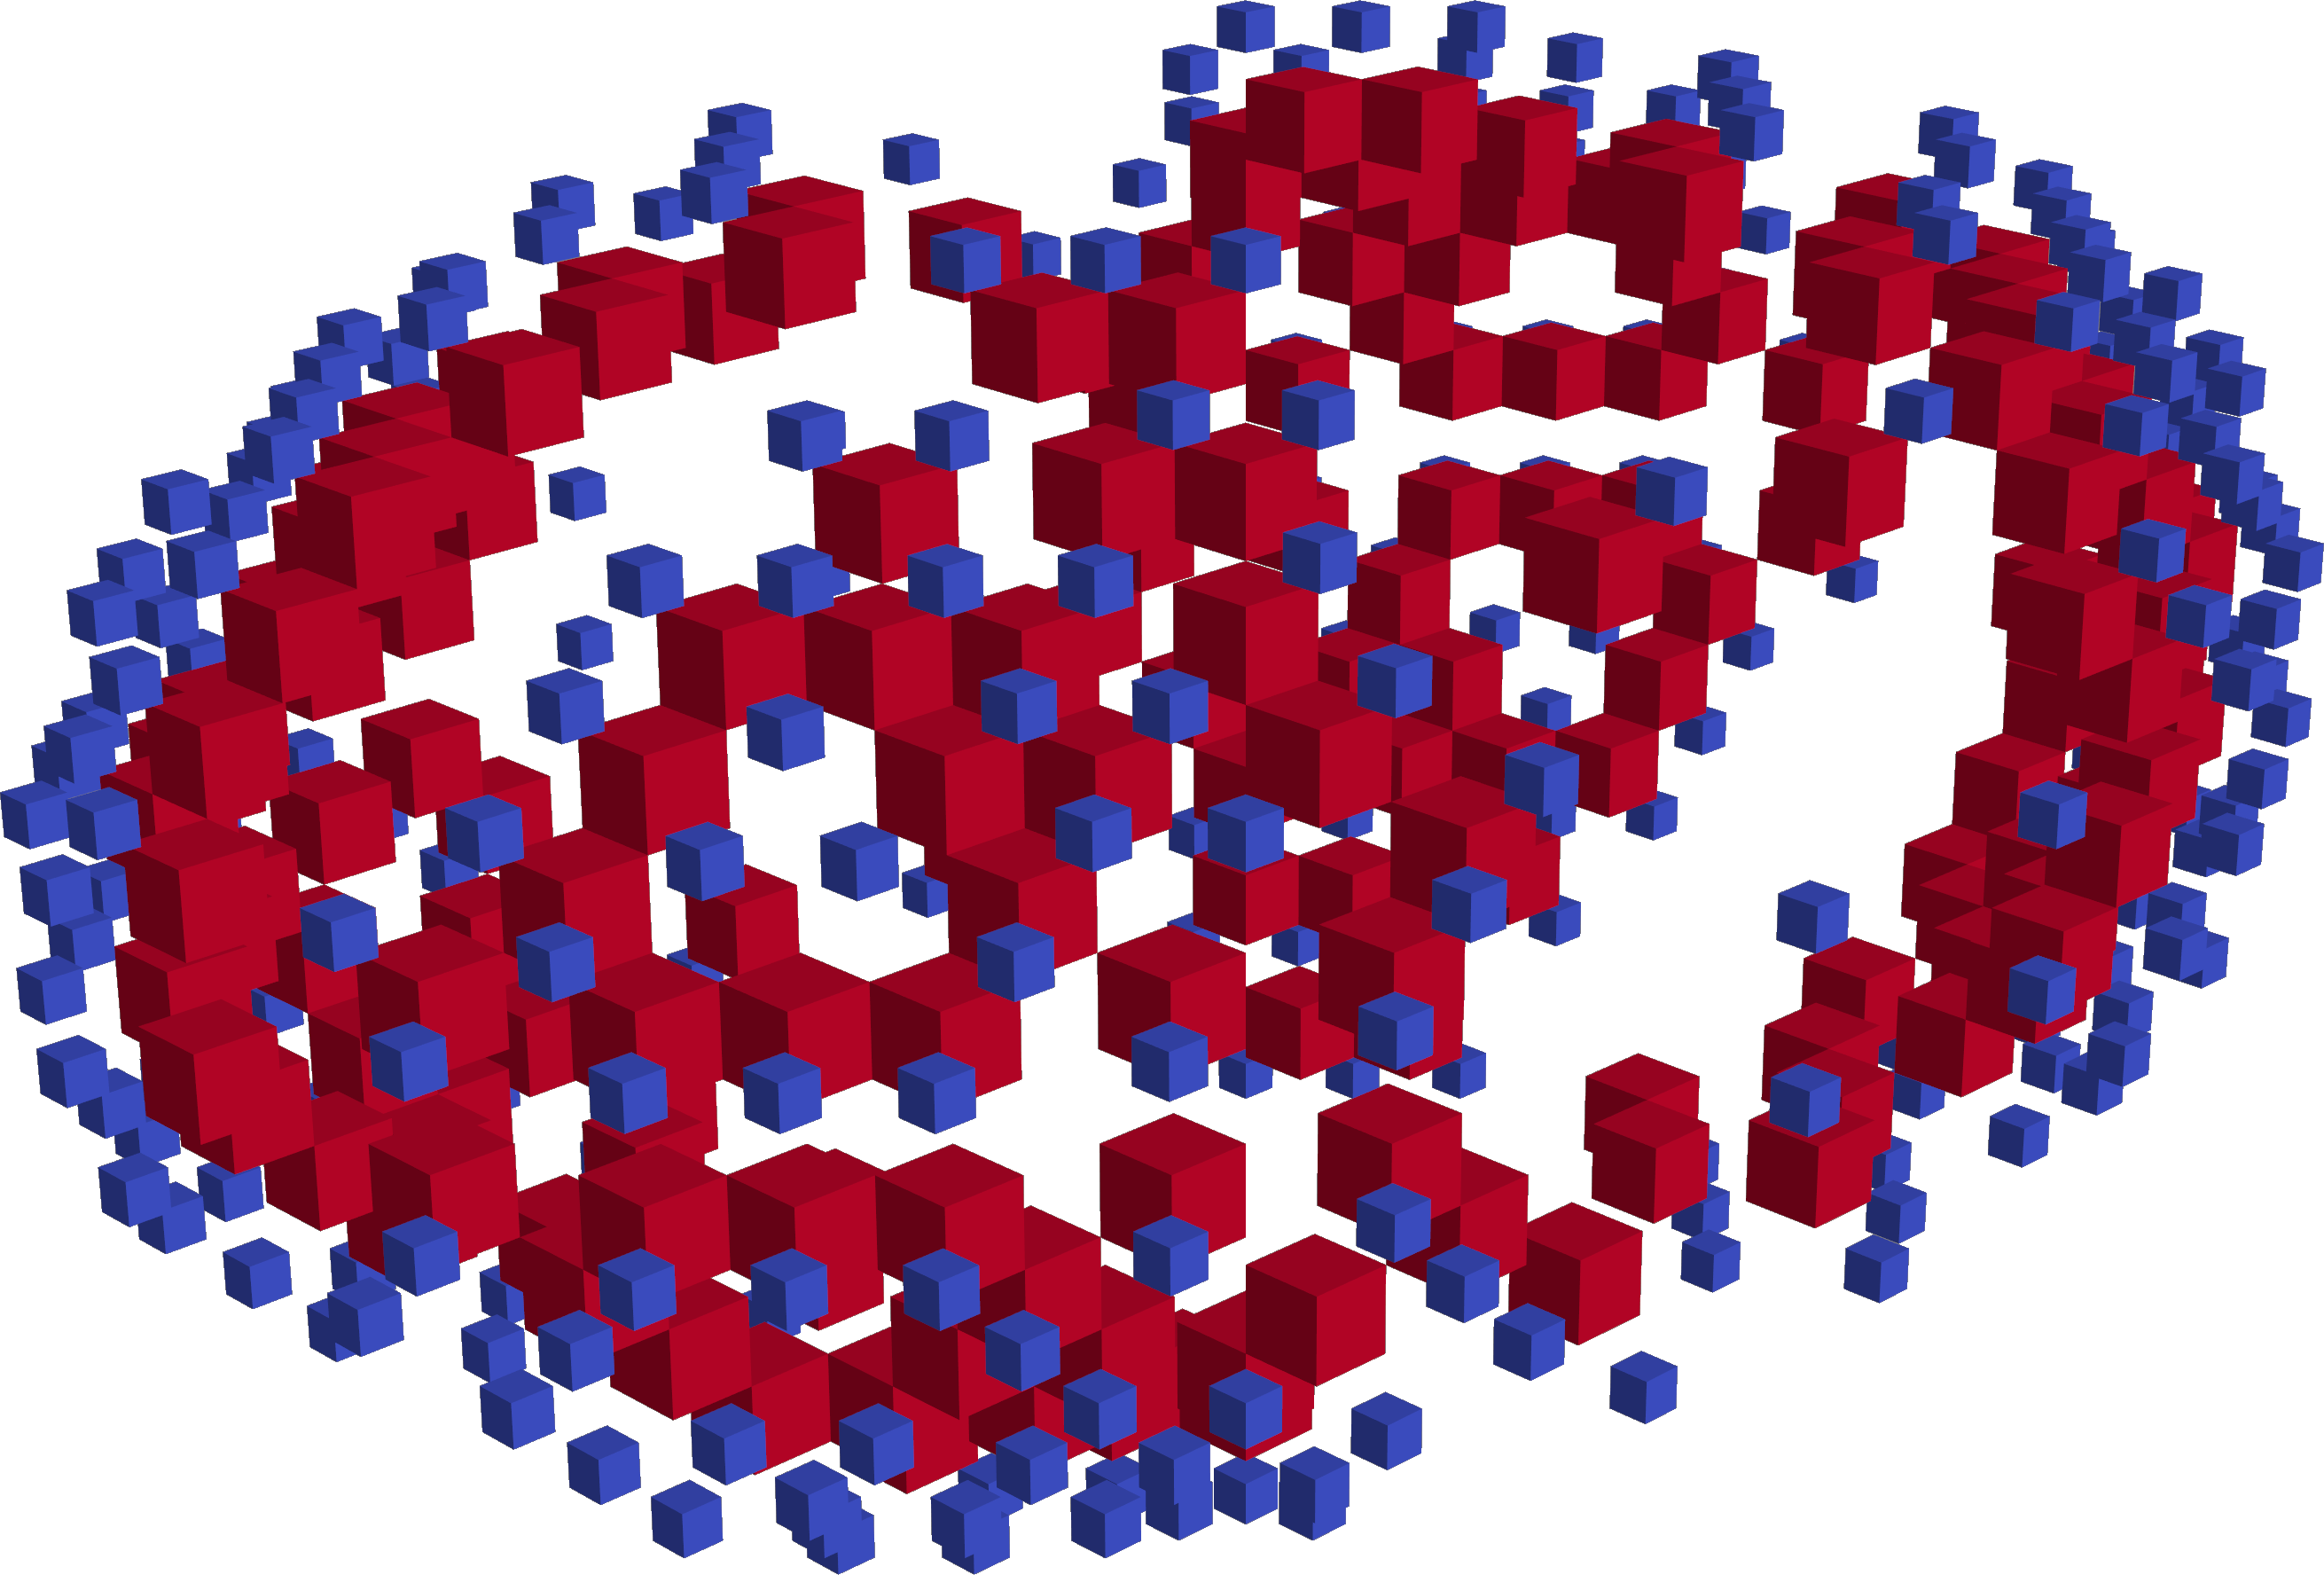
\includegraphics[width=\textwidth]{../images/3D/Ellipsoid_blocks_isolated_vertices.png}
    \caption{The outside (in blue) and inside (in red) corners.}
    \label{fig:Ellipsoid_blocks_isolated_vertices}
    \end{subfigure}
    \hfill
    \begin{subfigure}{.32\textwidth}
        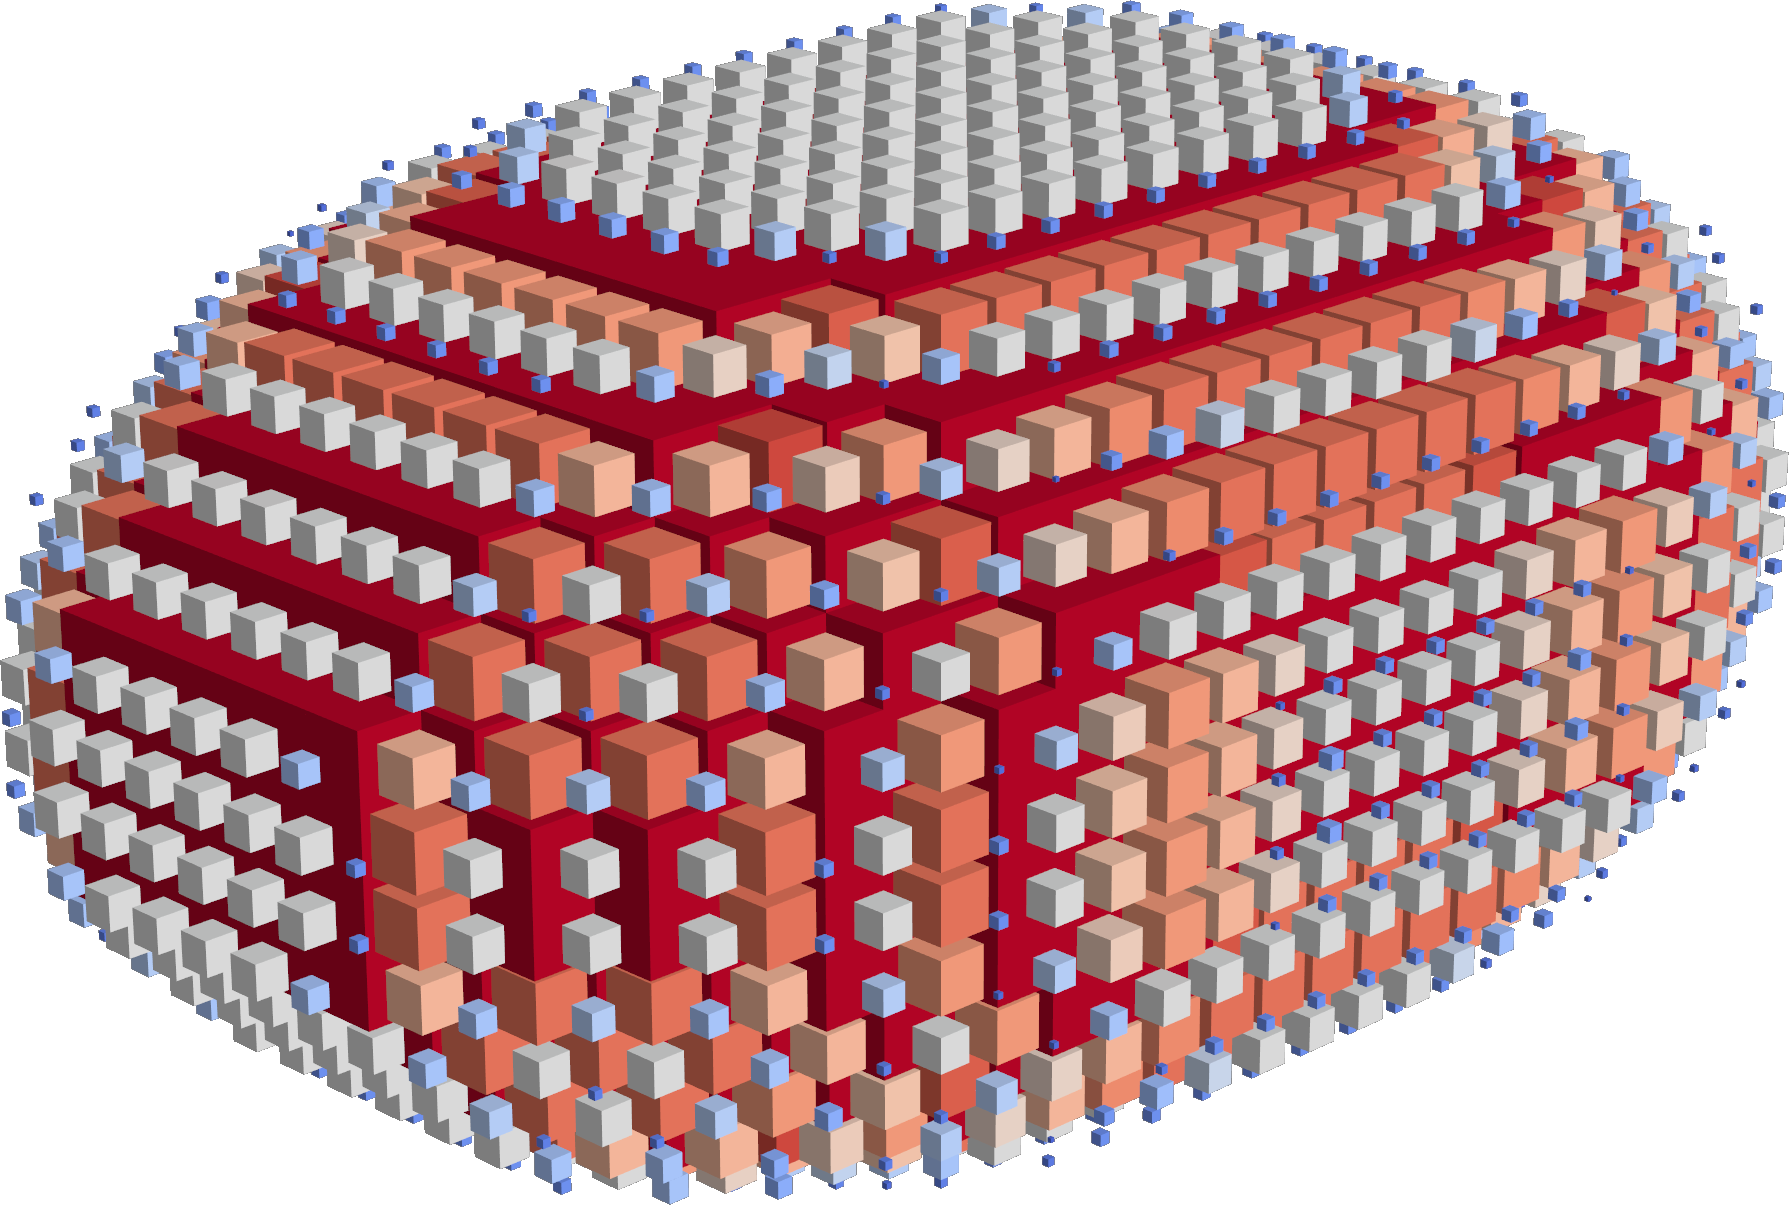
\includegraphics[width=\textwidth]{../images/3D/Ellipsoid_blocks_isolated_vertices_interpolated.png}
    \caption{The ellipsoid voxels with interpolated boundary region.}
    \label{fig:Ellipsoid_blocks_isolated_vertices_interpolated}
    \end{subfigure}
    \hfill
    \begin{subfigure}{.32\textwidth}
        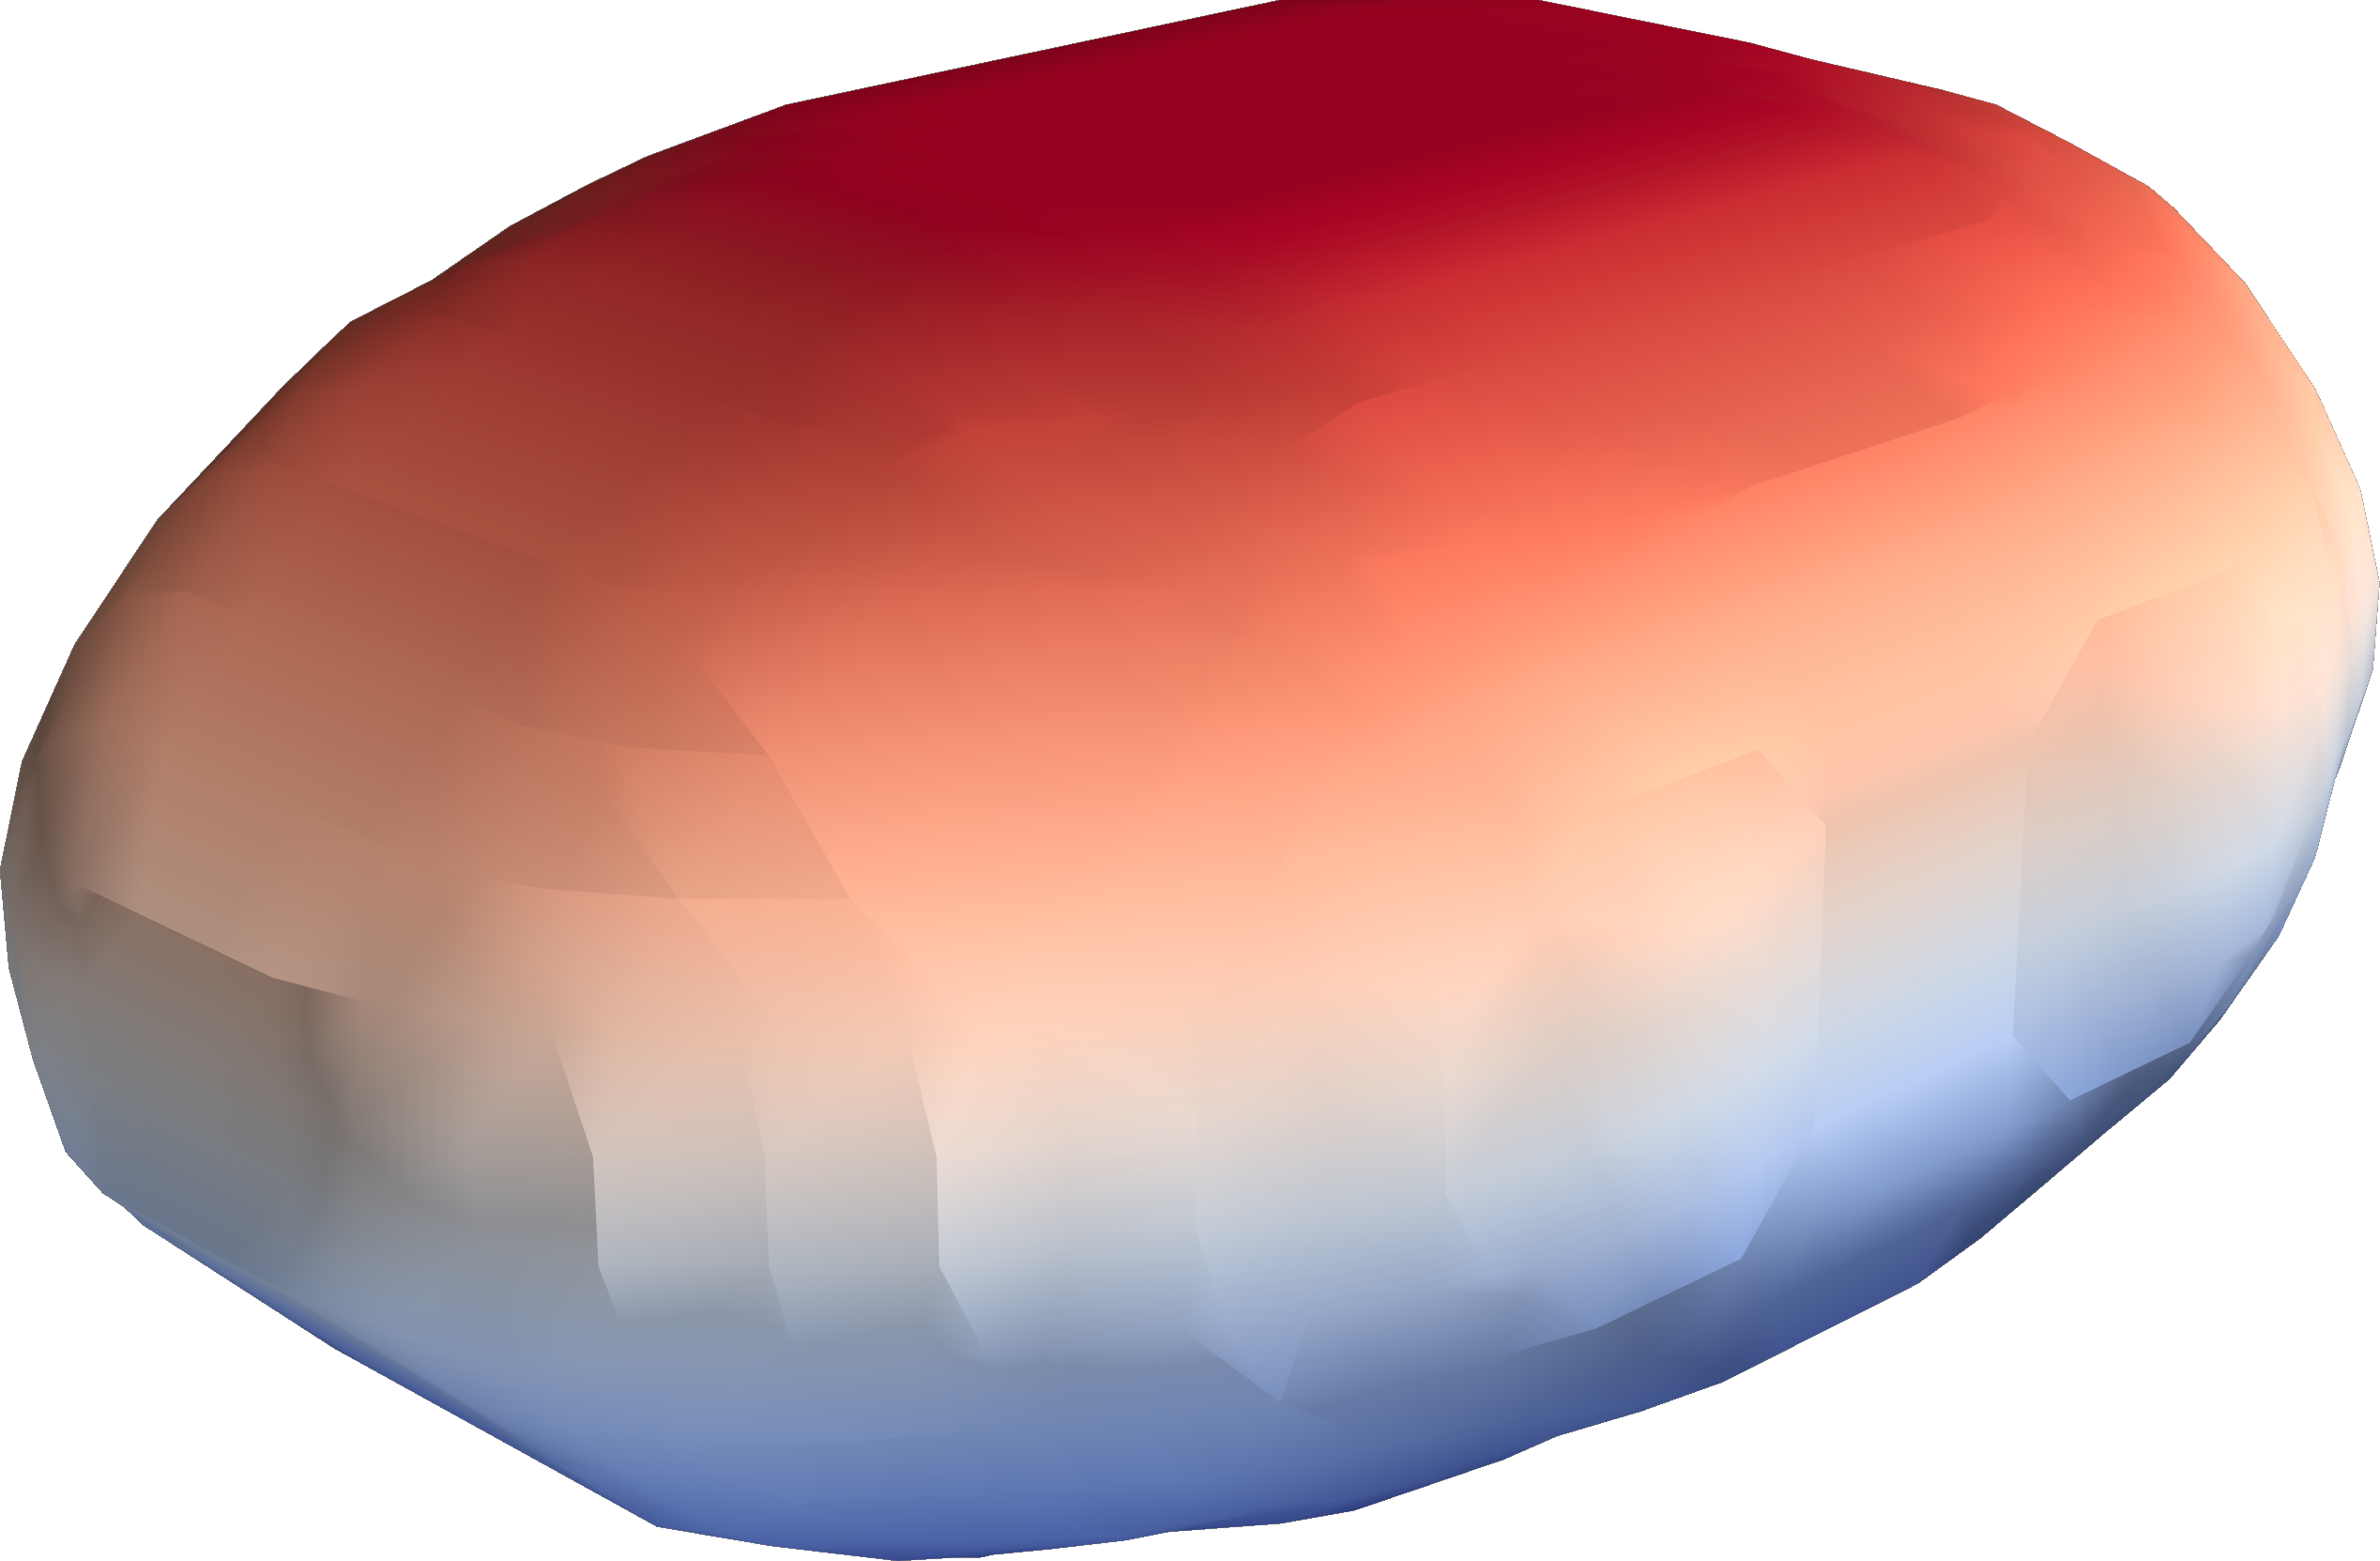
\includegraphics[width=\textwidth]{../images/3D/Ellipsoid_marching_squares_isolated_vertices.png}
    \caption{The triangular mesh produced by marching squares.}
    \label{fig:Ellipsoid_marching_squares_isolated_vertices}
    \end{subfigure}
    \caption{Illustration of contour interpolation using isolation of corner vertices with block size 2.}
    \label{fig:Ellipsoid_isolated_vertices}
\end{figure}

\begin{figure}[H]
    \centering
    \begin{subfigure}{.32\textwidth}
        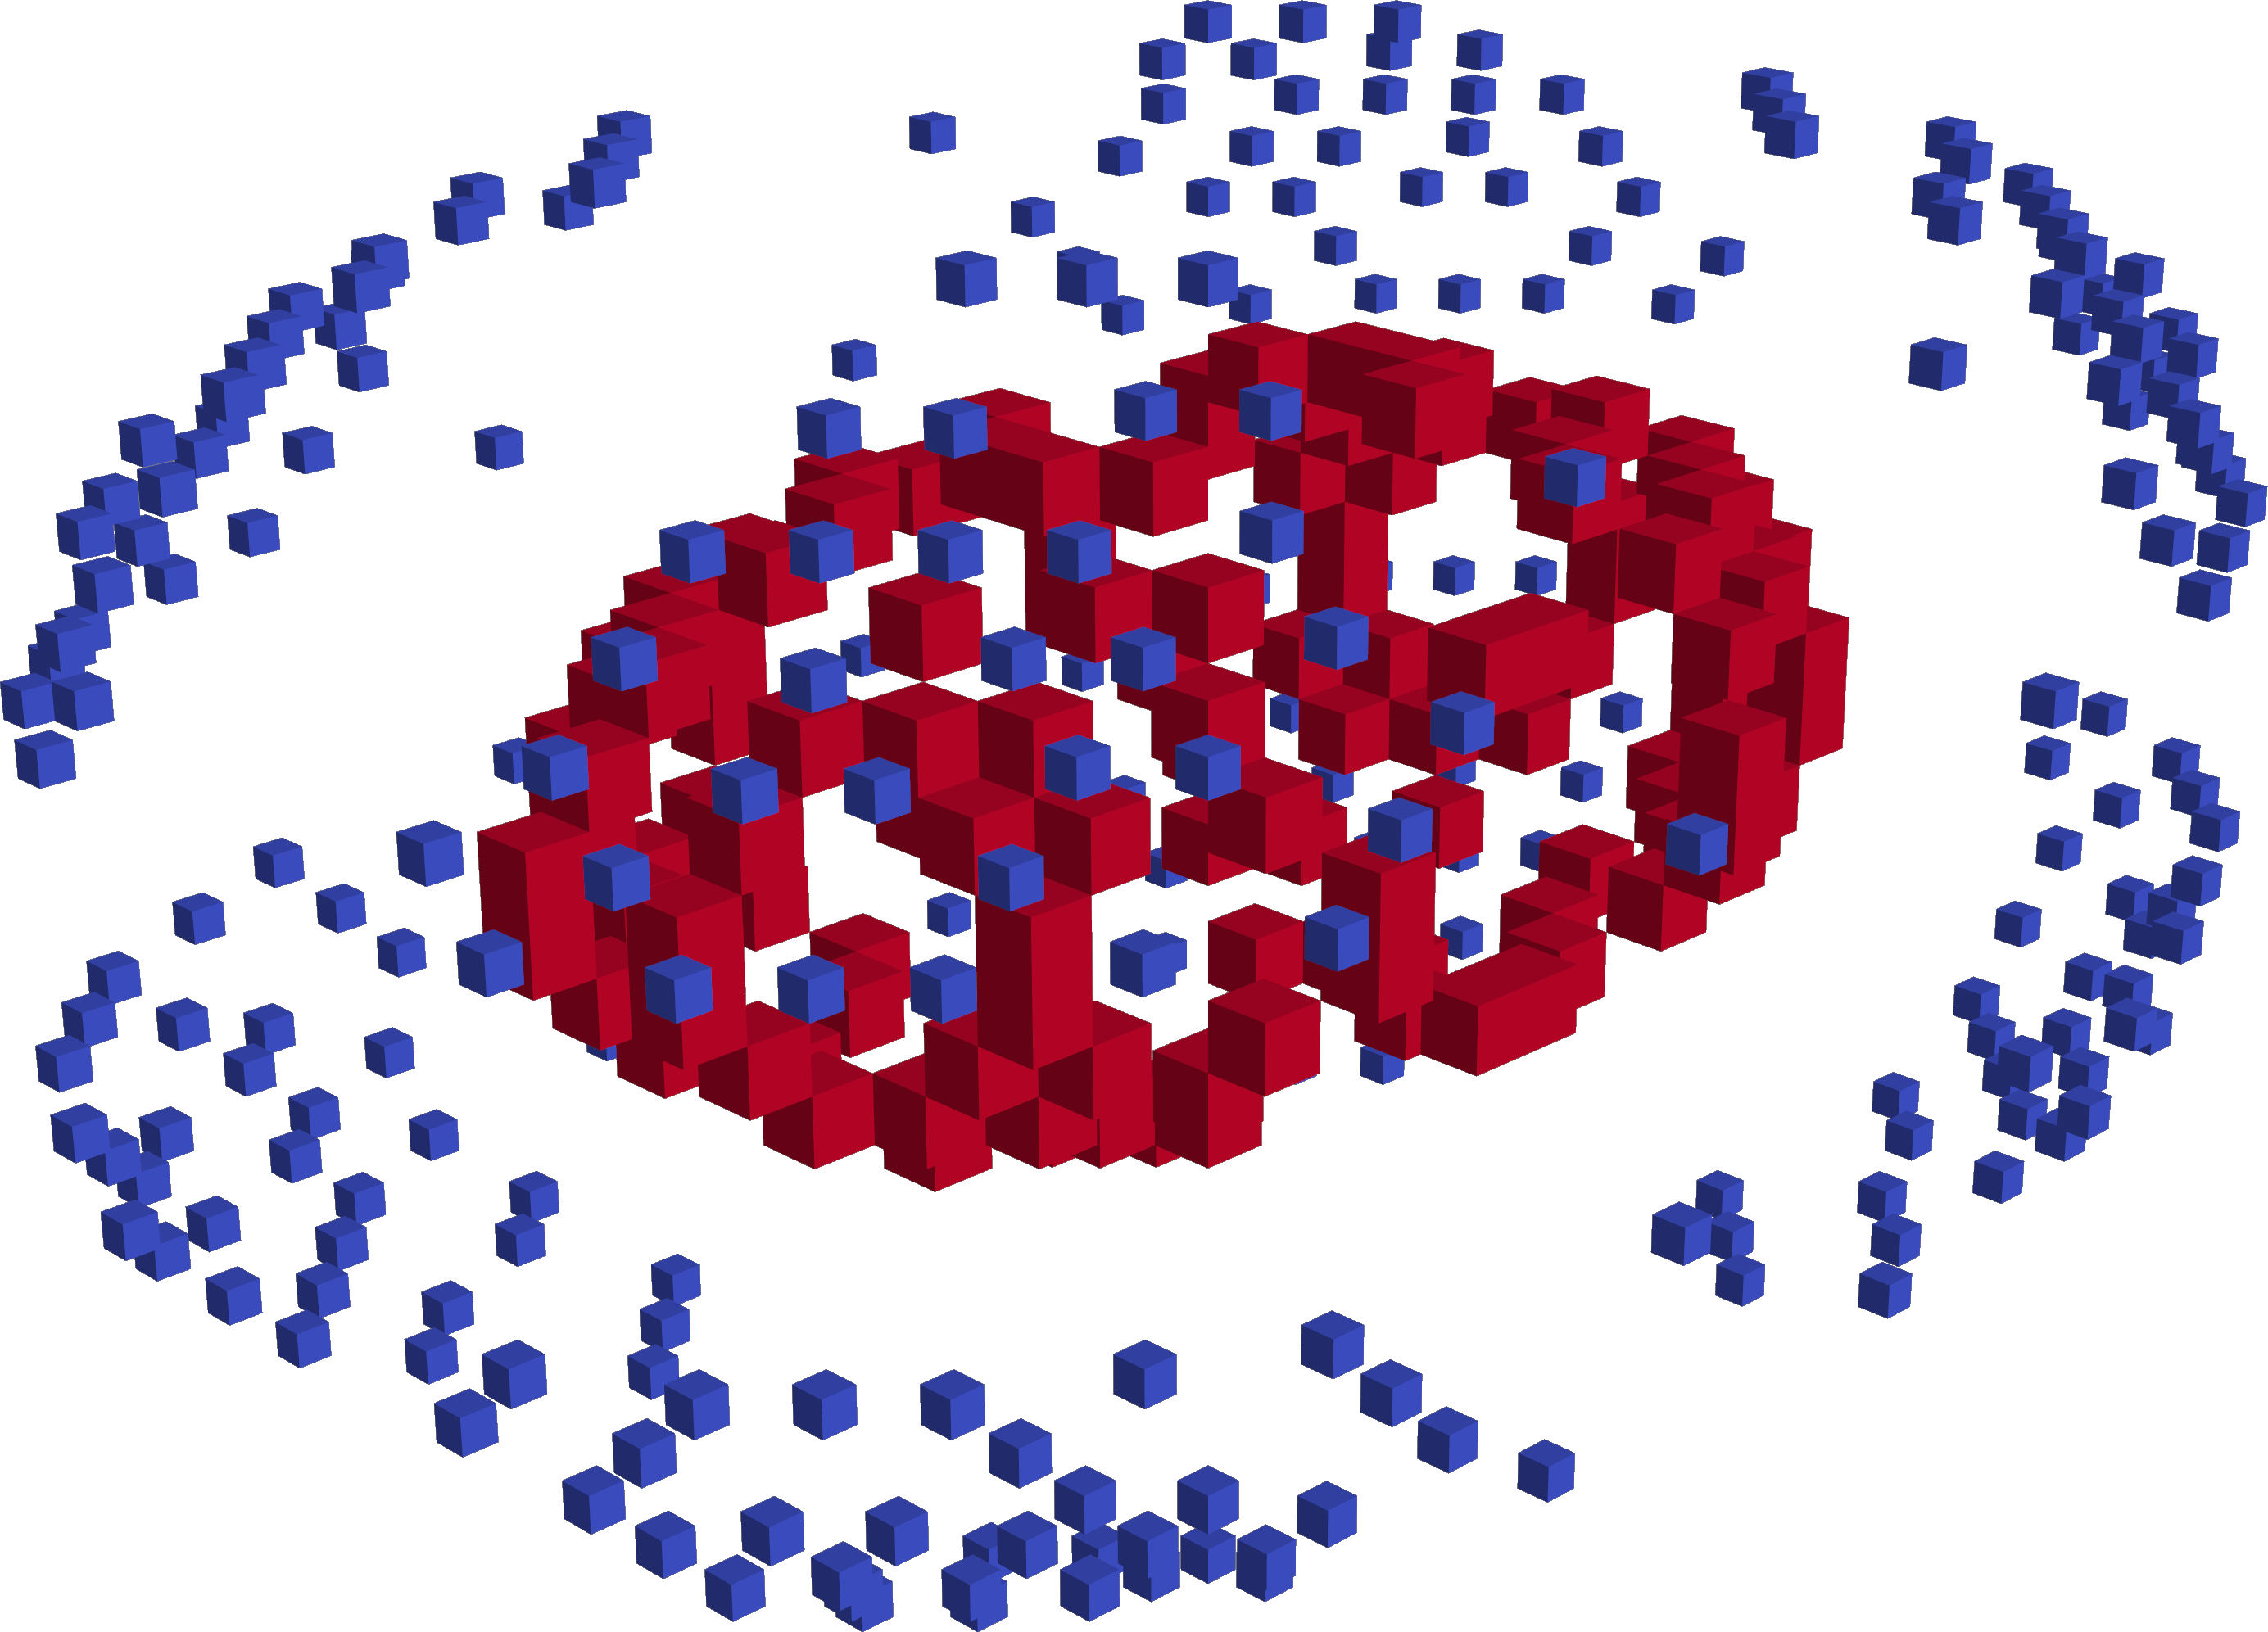
\includegraphics[width=\textwidth]{../images/3D/Ellipsoid_blocks_isolated_vertices_5.png}
    \caption{The outside (in blue) and inside (in red) corners.}
    \label{fig:Ellipsoid_blocks_isolated_vertices_5}
    \end{subfigure}
    \hfill
    \begin{subfigure}{.32\textwidth}
        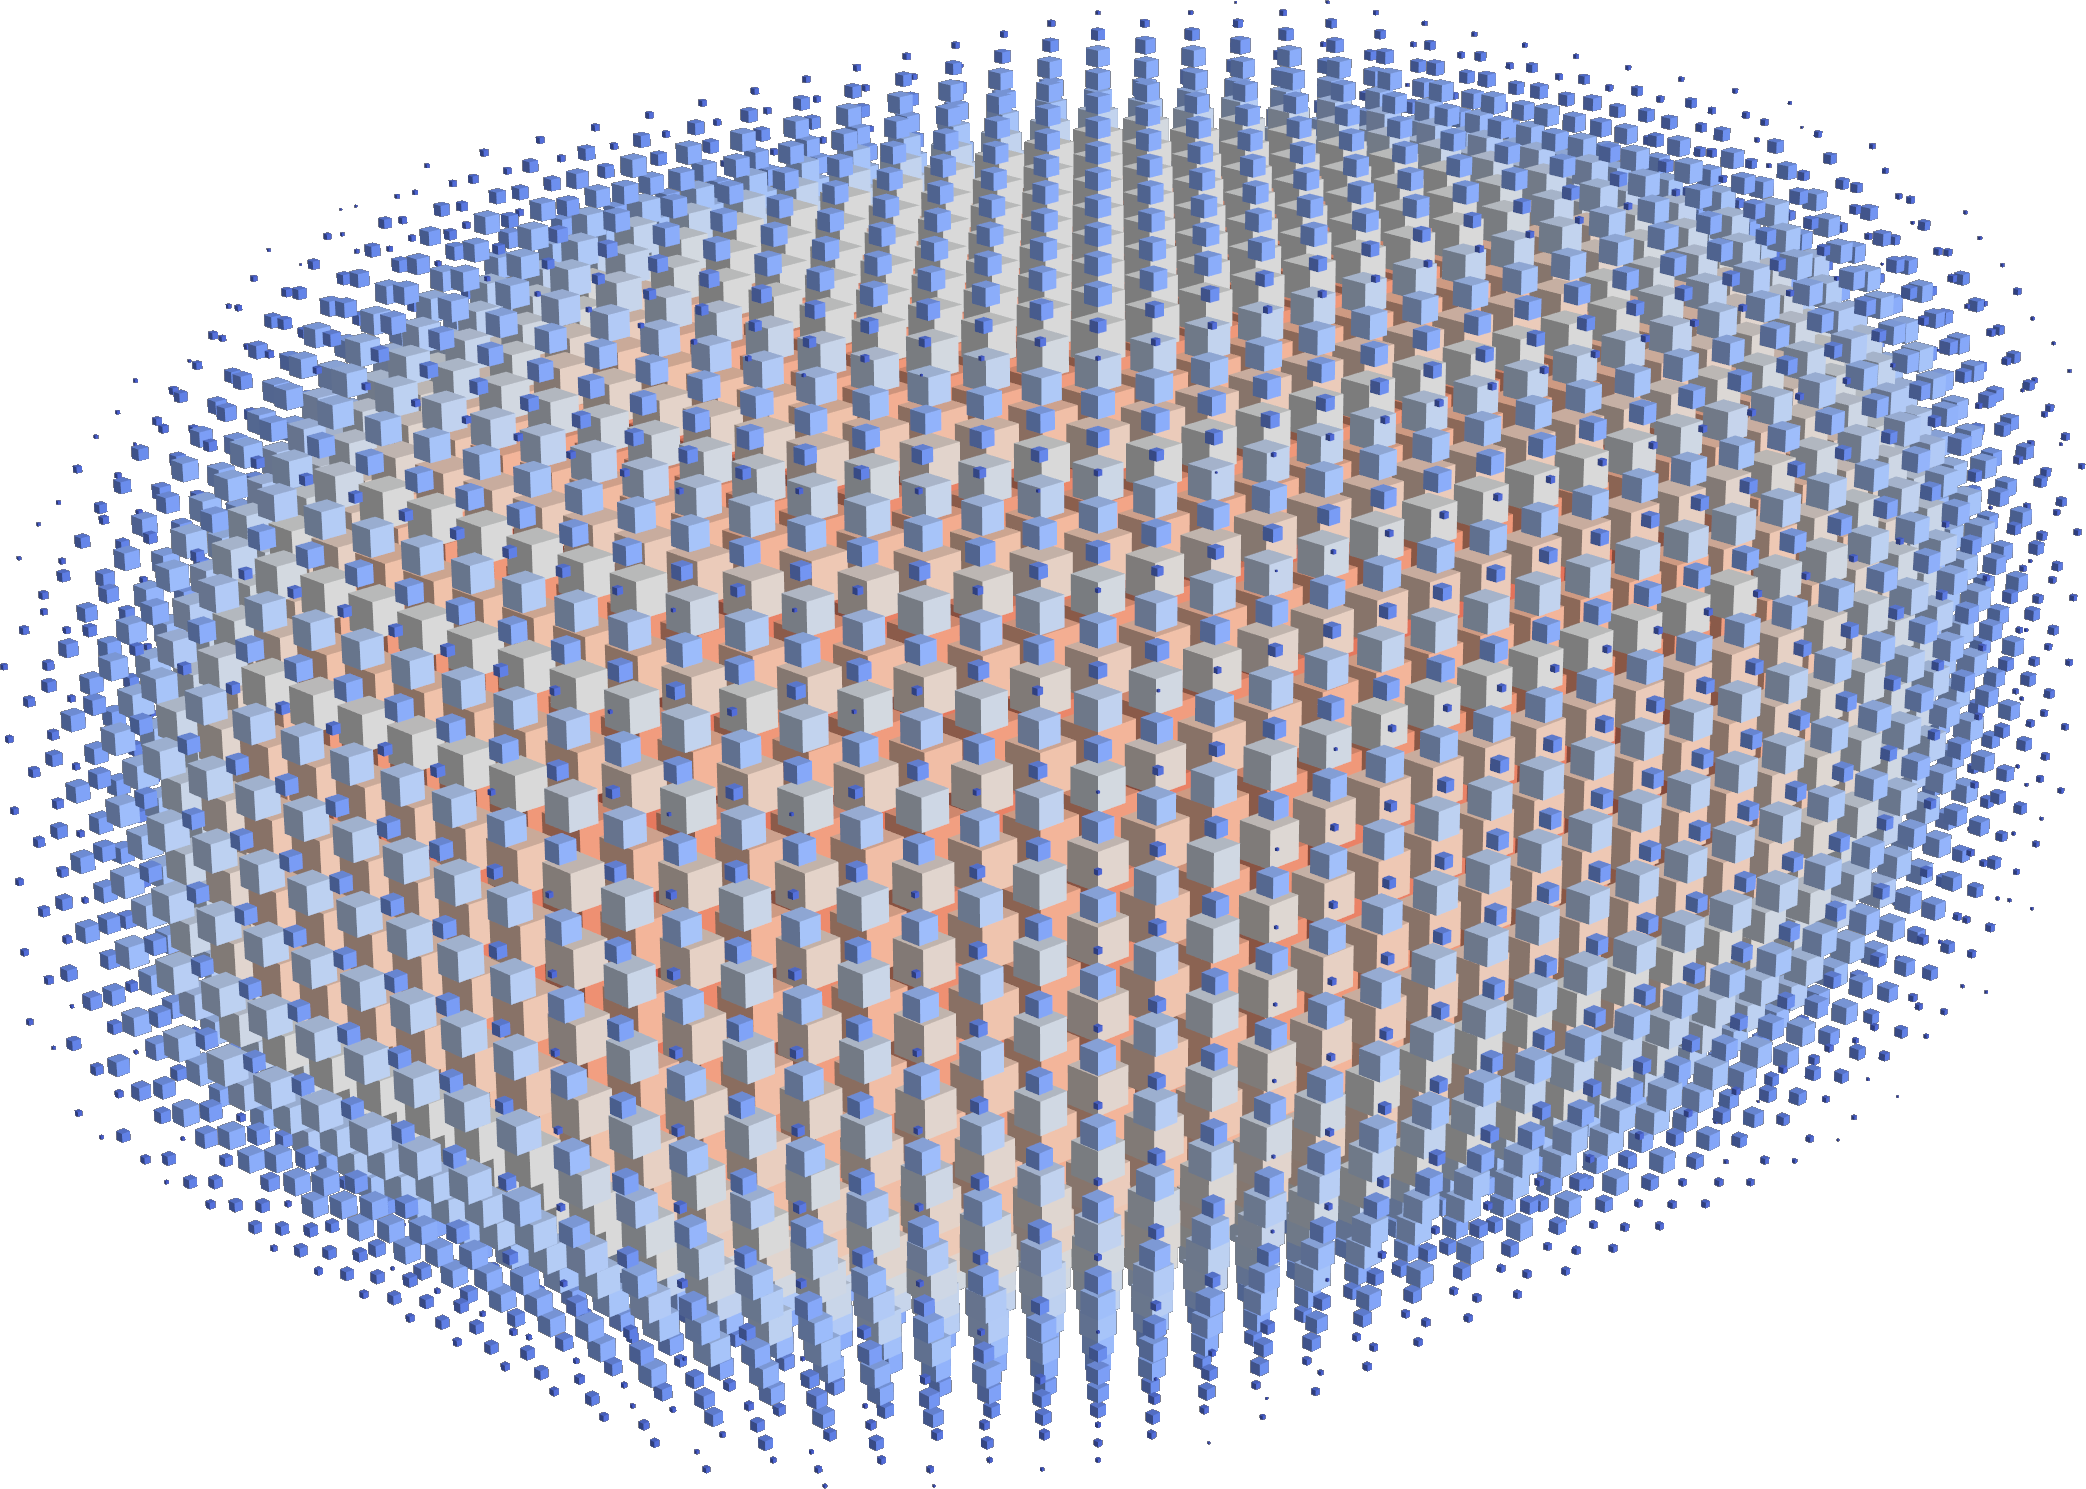
\includegraphics[width=\textwidth]{../images/3D/Ellipsoid_blocks_isolated_vertices_interpolated_5.png}
    \caption{The ellipsoid voxels with interpolated boundary region.}
    \label{fig:Ellipsoid_blocks_isolated_vertices_interpolated_5}
    \end{subfigure}
    \hfill
    \begin{subfigure}{.32\textwidth}
        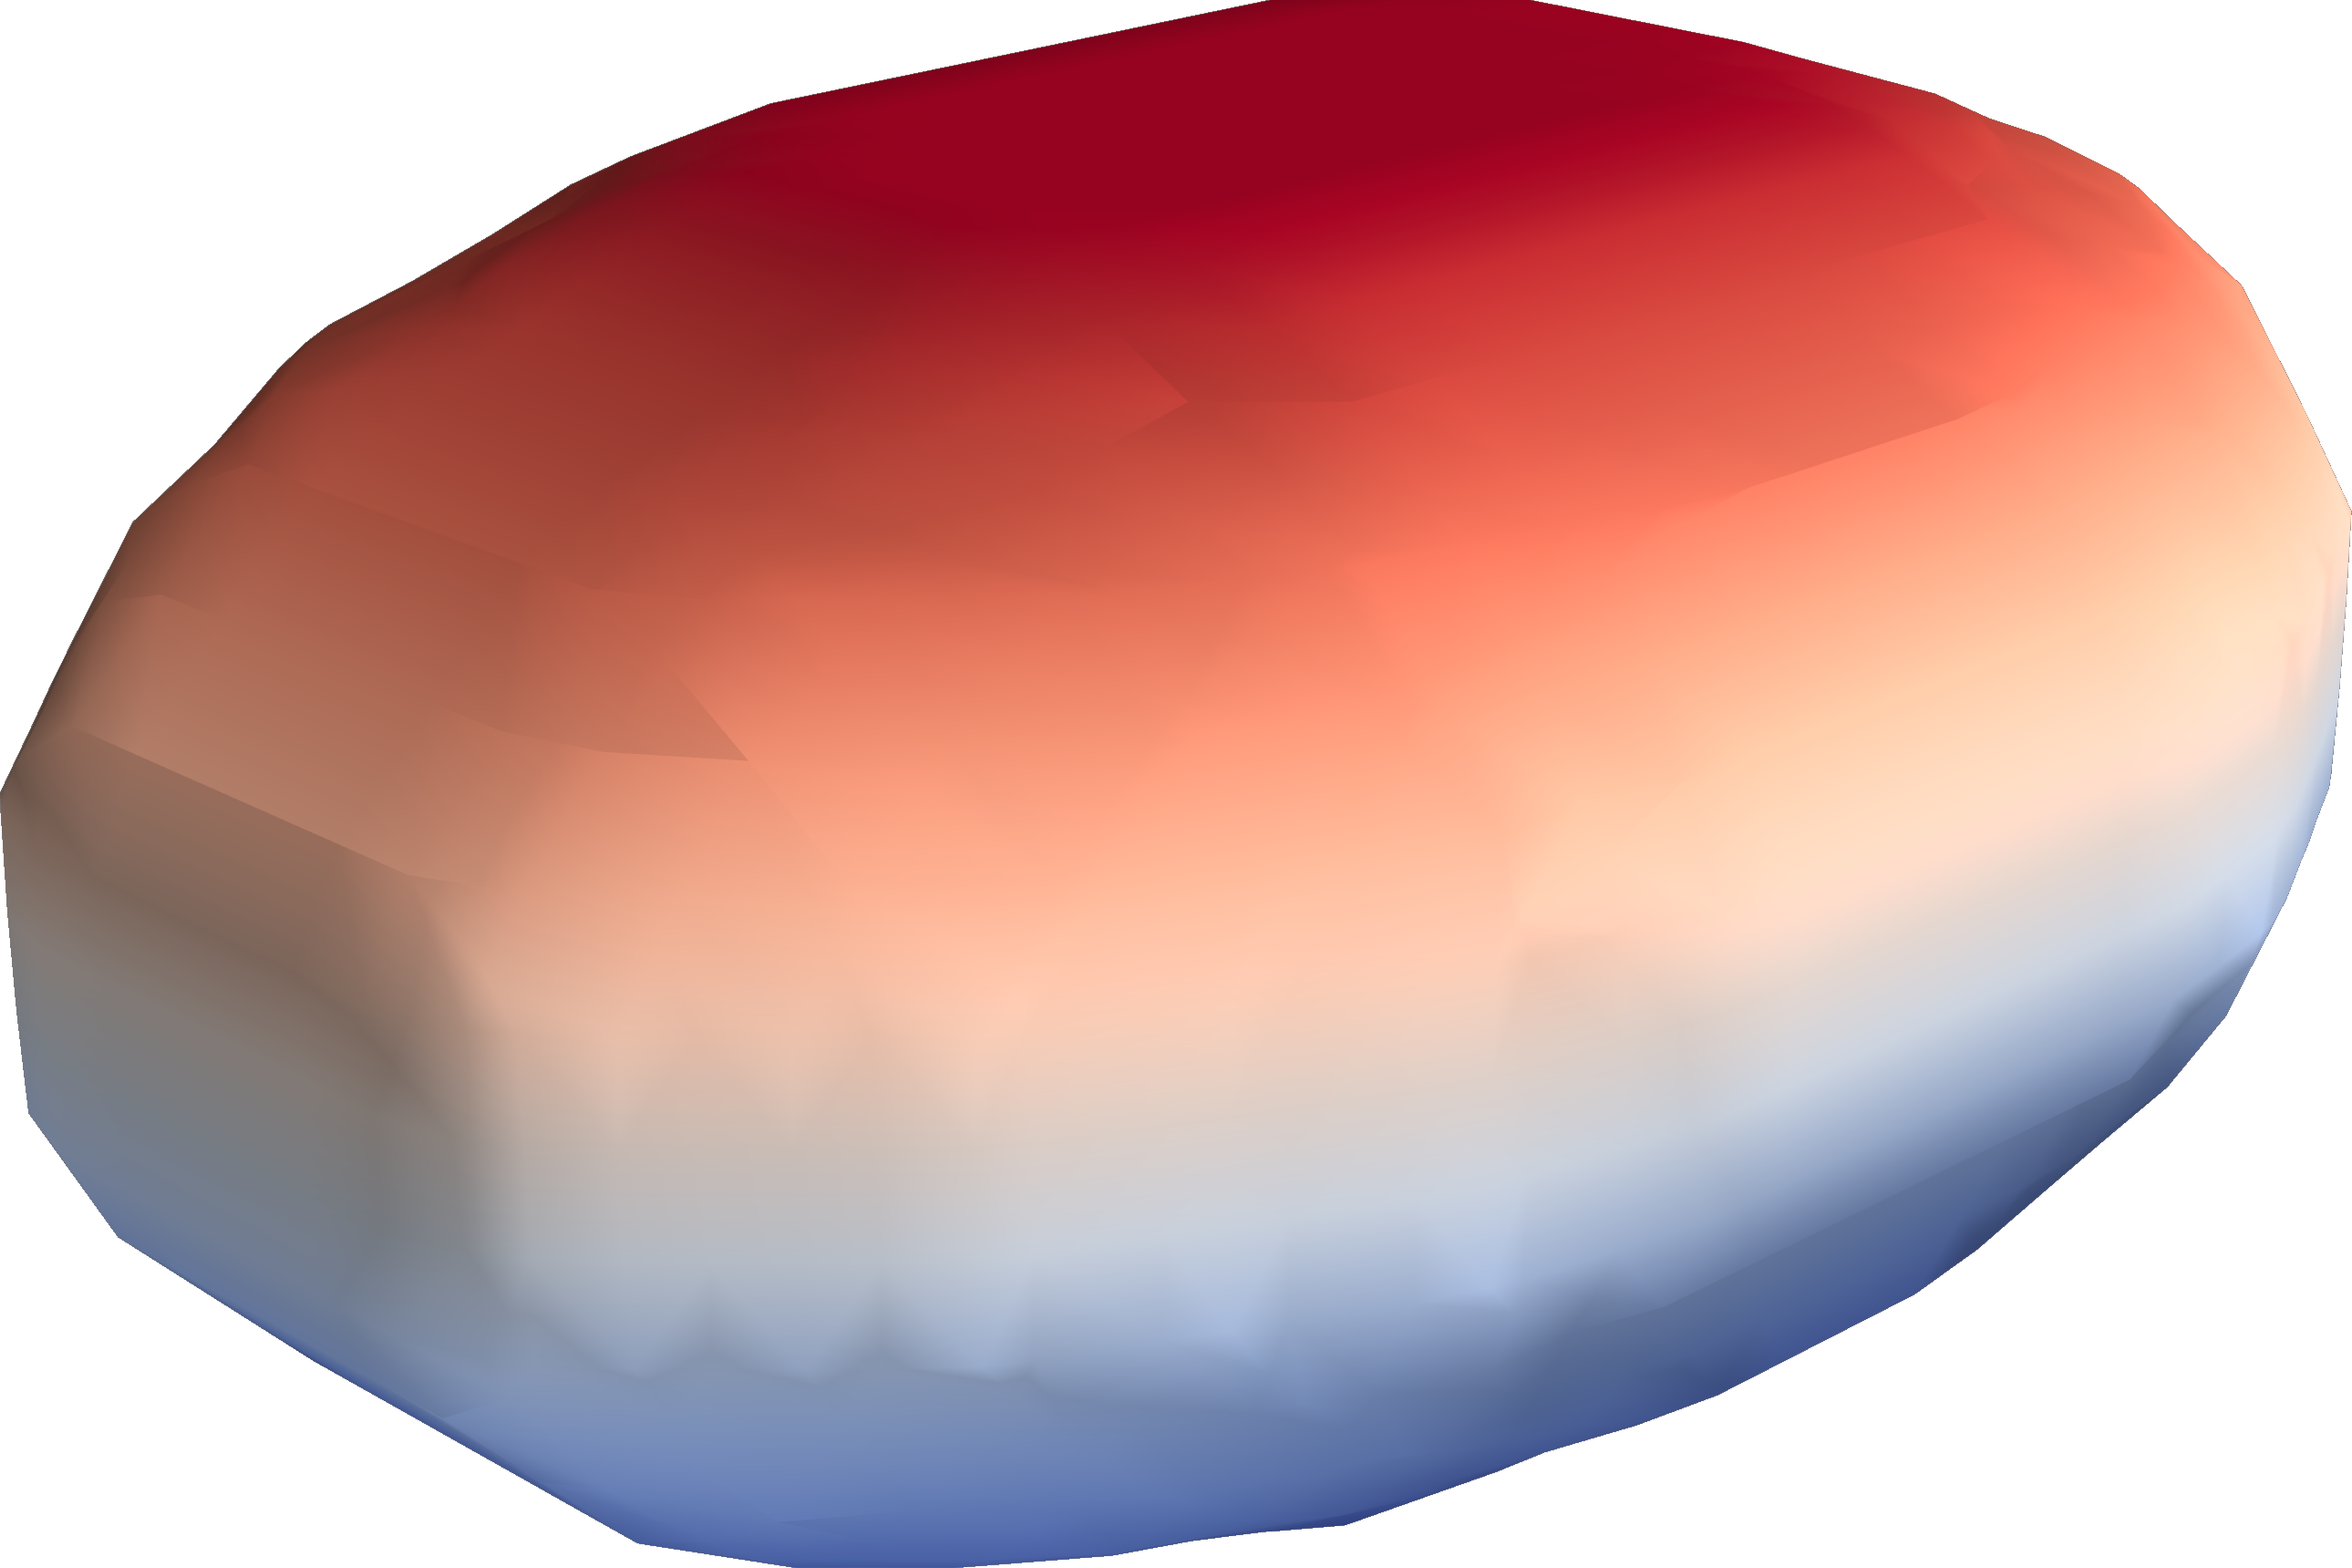
\includegraphics[width=\textwidth]{../images/3D/Ellipsoid_marching_squares_isolated_vertices_5.png}
    \caption{The triangular mesh produced by marching squares.}
    \label{fig:Ellipsoid_marching_squares_isolated_vertices_5}
    \end{subfigure}
    \caption{Illustration of contour interpolation using isolation of corner vertices with block size 5.}
    \label{fig:Ellipsoid_isolated_vertices_5}
\end{figure}

The mesh shown in Figure \ref{fig:Ellipsoid_isolated_vertices} was produced by using block size of 2. When compared to the mesh in Figure \ref{fig:Ellipsoid_block_avg} produced by block averaging with block size 2, we can notice that this method creates smoother contours.

However, it is also noticeable that this method does not preserve shapes exactly. As the block size is increased, the ellipsoid is being deformed into a cuboid, which is noticeable in Figure \ref{fig:Ellipsoid_isolated_vertices_5}. Therefore increasing the block size in this case does not always produce better looking results.

Another noteworthy observation is that this algorithm would not work very well in the absence of \textit{internal} vertices. For example, applying this algorithm to a cuboid would make the boundary region of the cuboid vanish. This is however quite an edge case, as any other object shape does contain \textit{internal} vertices, and applying this algorithm would not be advantageous at all if we knew that the object is a cuboid beforehand.

\section{Convolution with Gaussian Kernel}\label{sec:gaussian_kernel}

We have touched the idea of convolution in Section \ref{sec:block_avg}. Instead of using a uniform kernel, we can use any kernel that might produce better looking results. A very common kernel for smoothing data and images is the Gaussian kernel. In image and signal processing, the convolution with Gaussian kernel is called the Gaussian filter and is used very widely. We can see the illustration of the Gaussian kernel compared to uniform kernel in Figure \ref{fig:kernel_comparison}, and it's application on the ellipsoid example in Figure \ref{fig:Ellipsoid_gaussian}.
\begin{figure}[H]
    \centering
    \includesvg[width=0.49\textwidth]{../images/3D/Kernels.svg}
    \caption{Comparison of uniform and Gaussian kernels with width 21.}
    \label{fig:kernel_comparison}
\end{figure}

\begin{figure}[H]
    \centering
    \begin{subfigure}{.49\textwidth}
        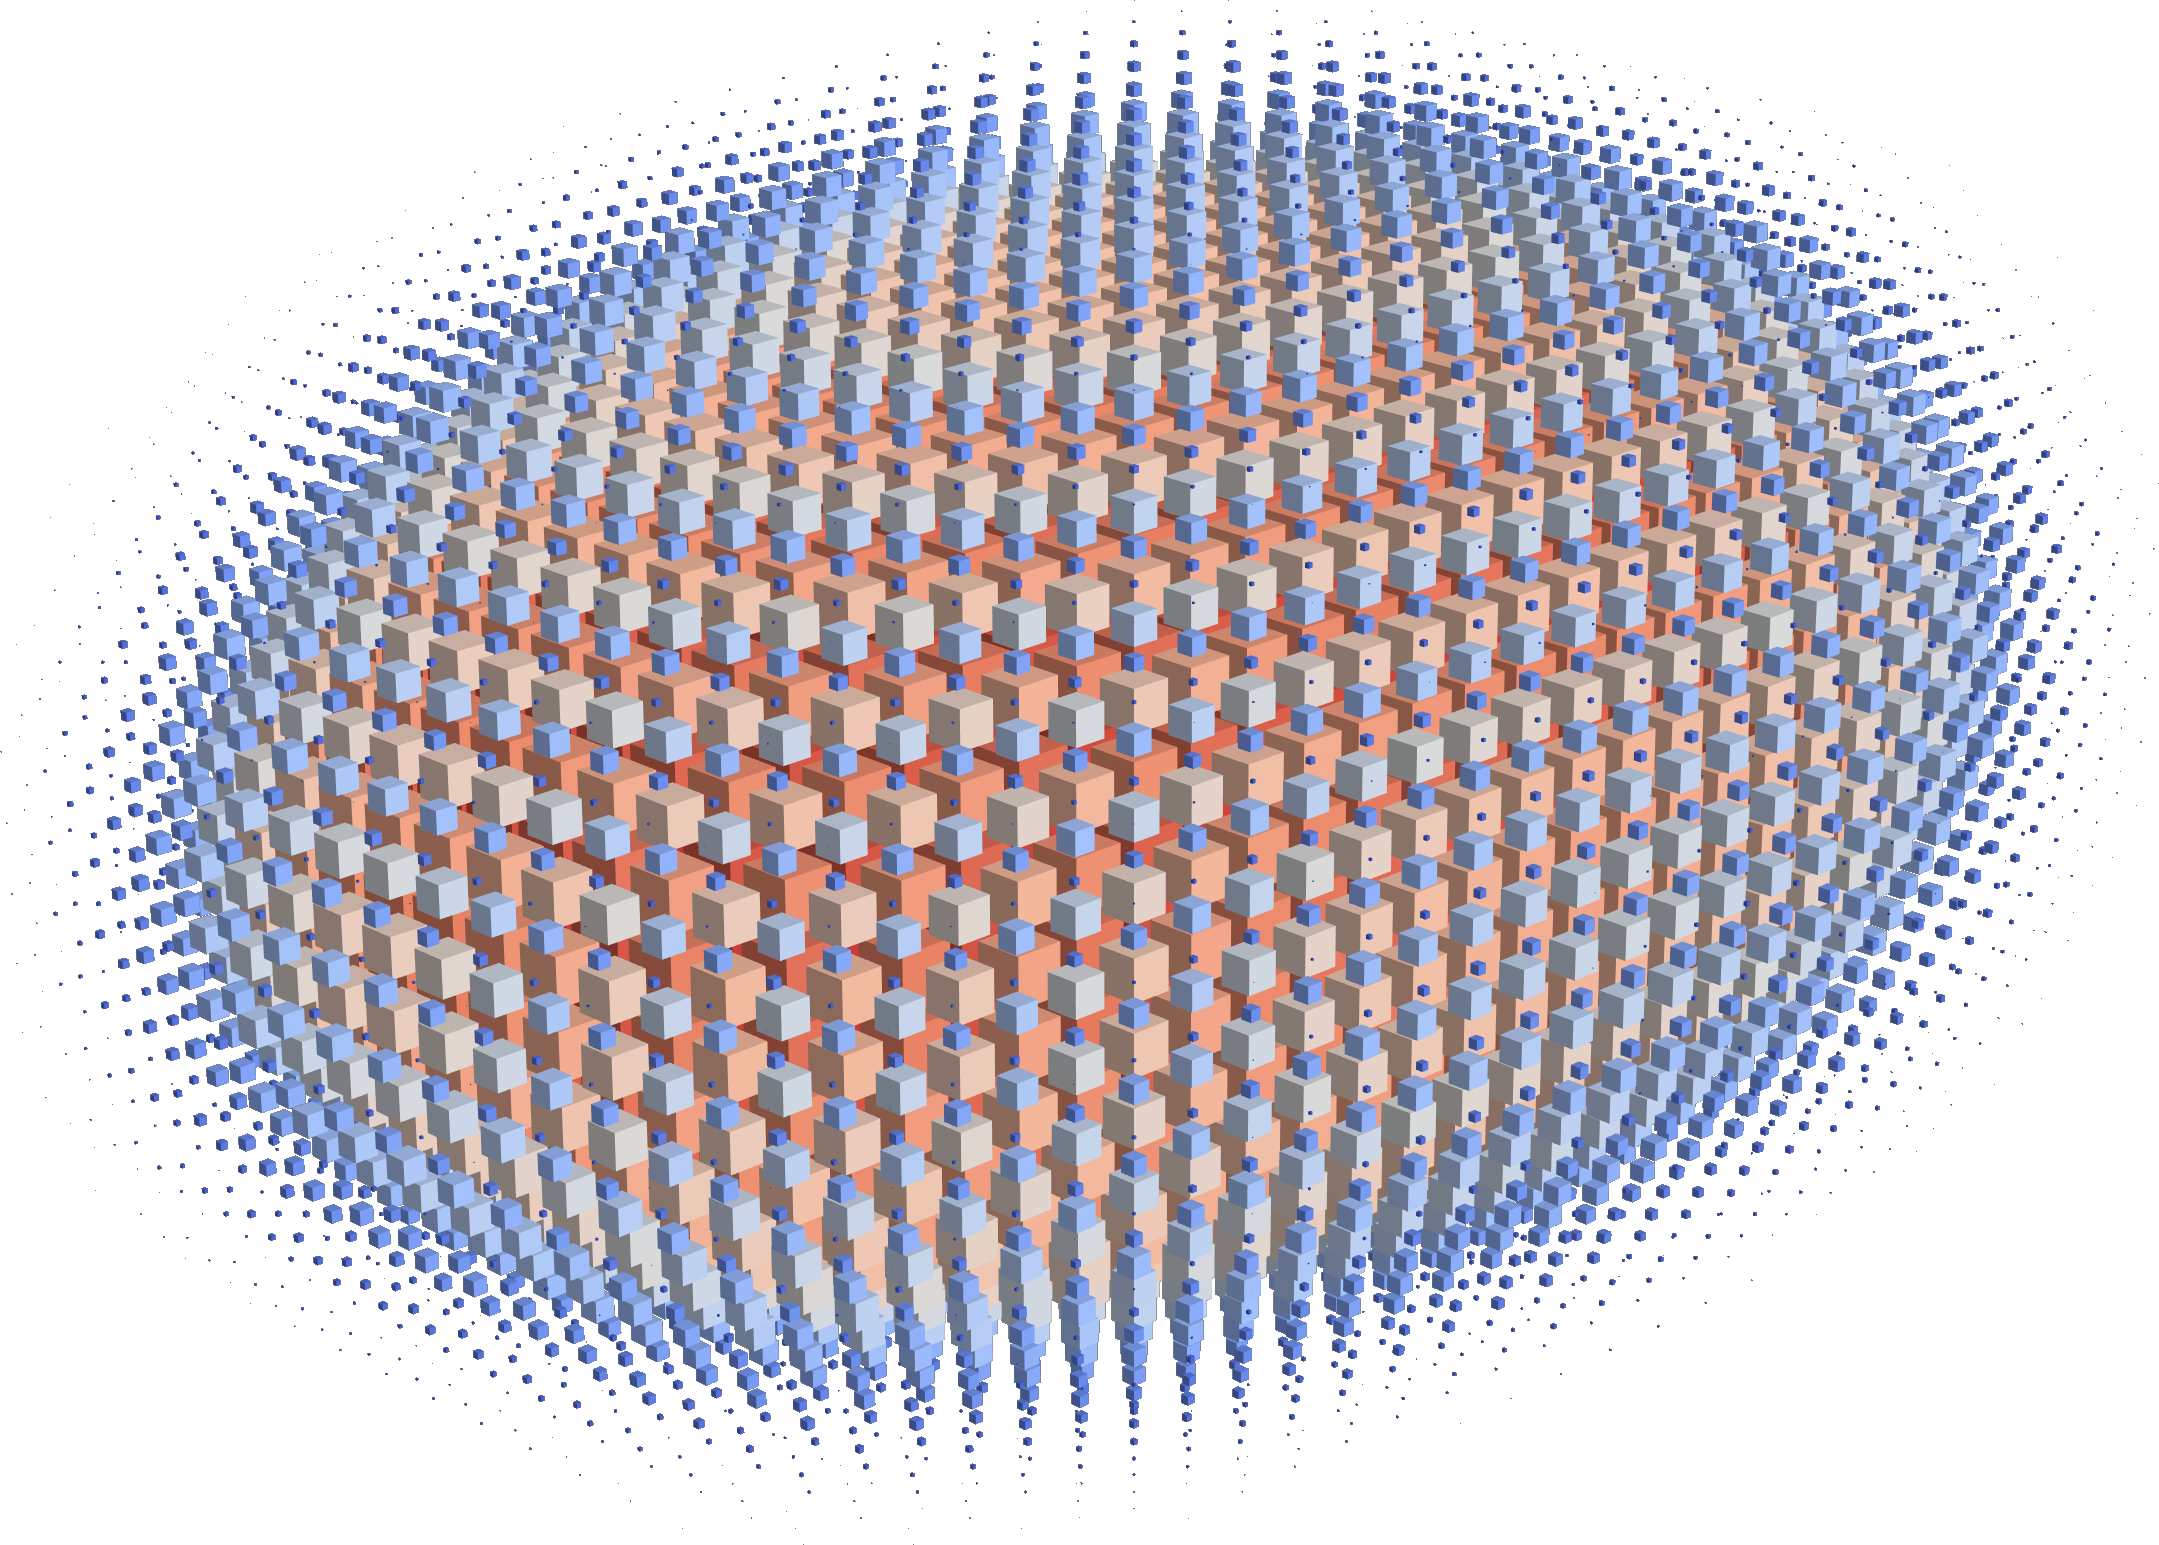
\includegraphics[width=\textwidth]{../images/3D/Ellipsoid_blocks_gaussian.png}
    \caption{The data voxels rendered directly.}
    \label{fig:Ellipsoid_blocks_gaussian}
    \end{subfigure}
    \hfill
    \begin{subfigure}{.49\textwidth}
        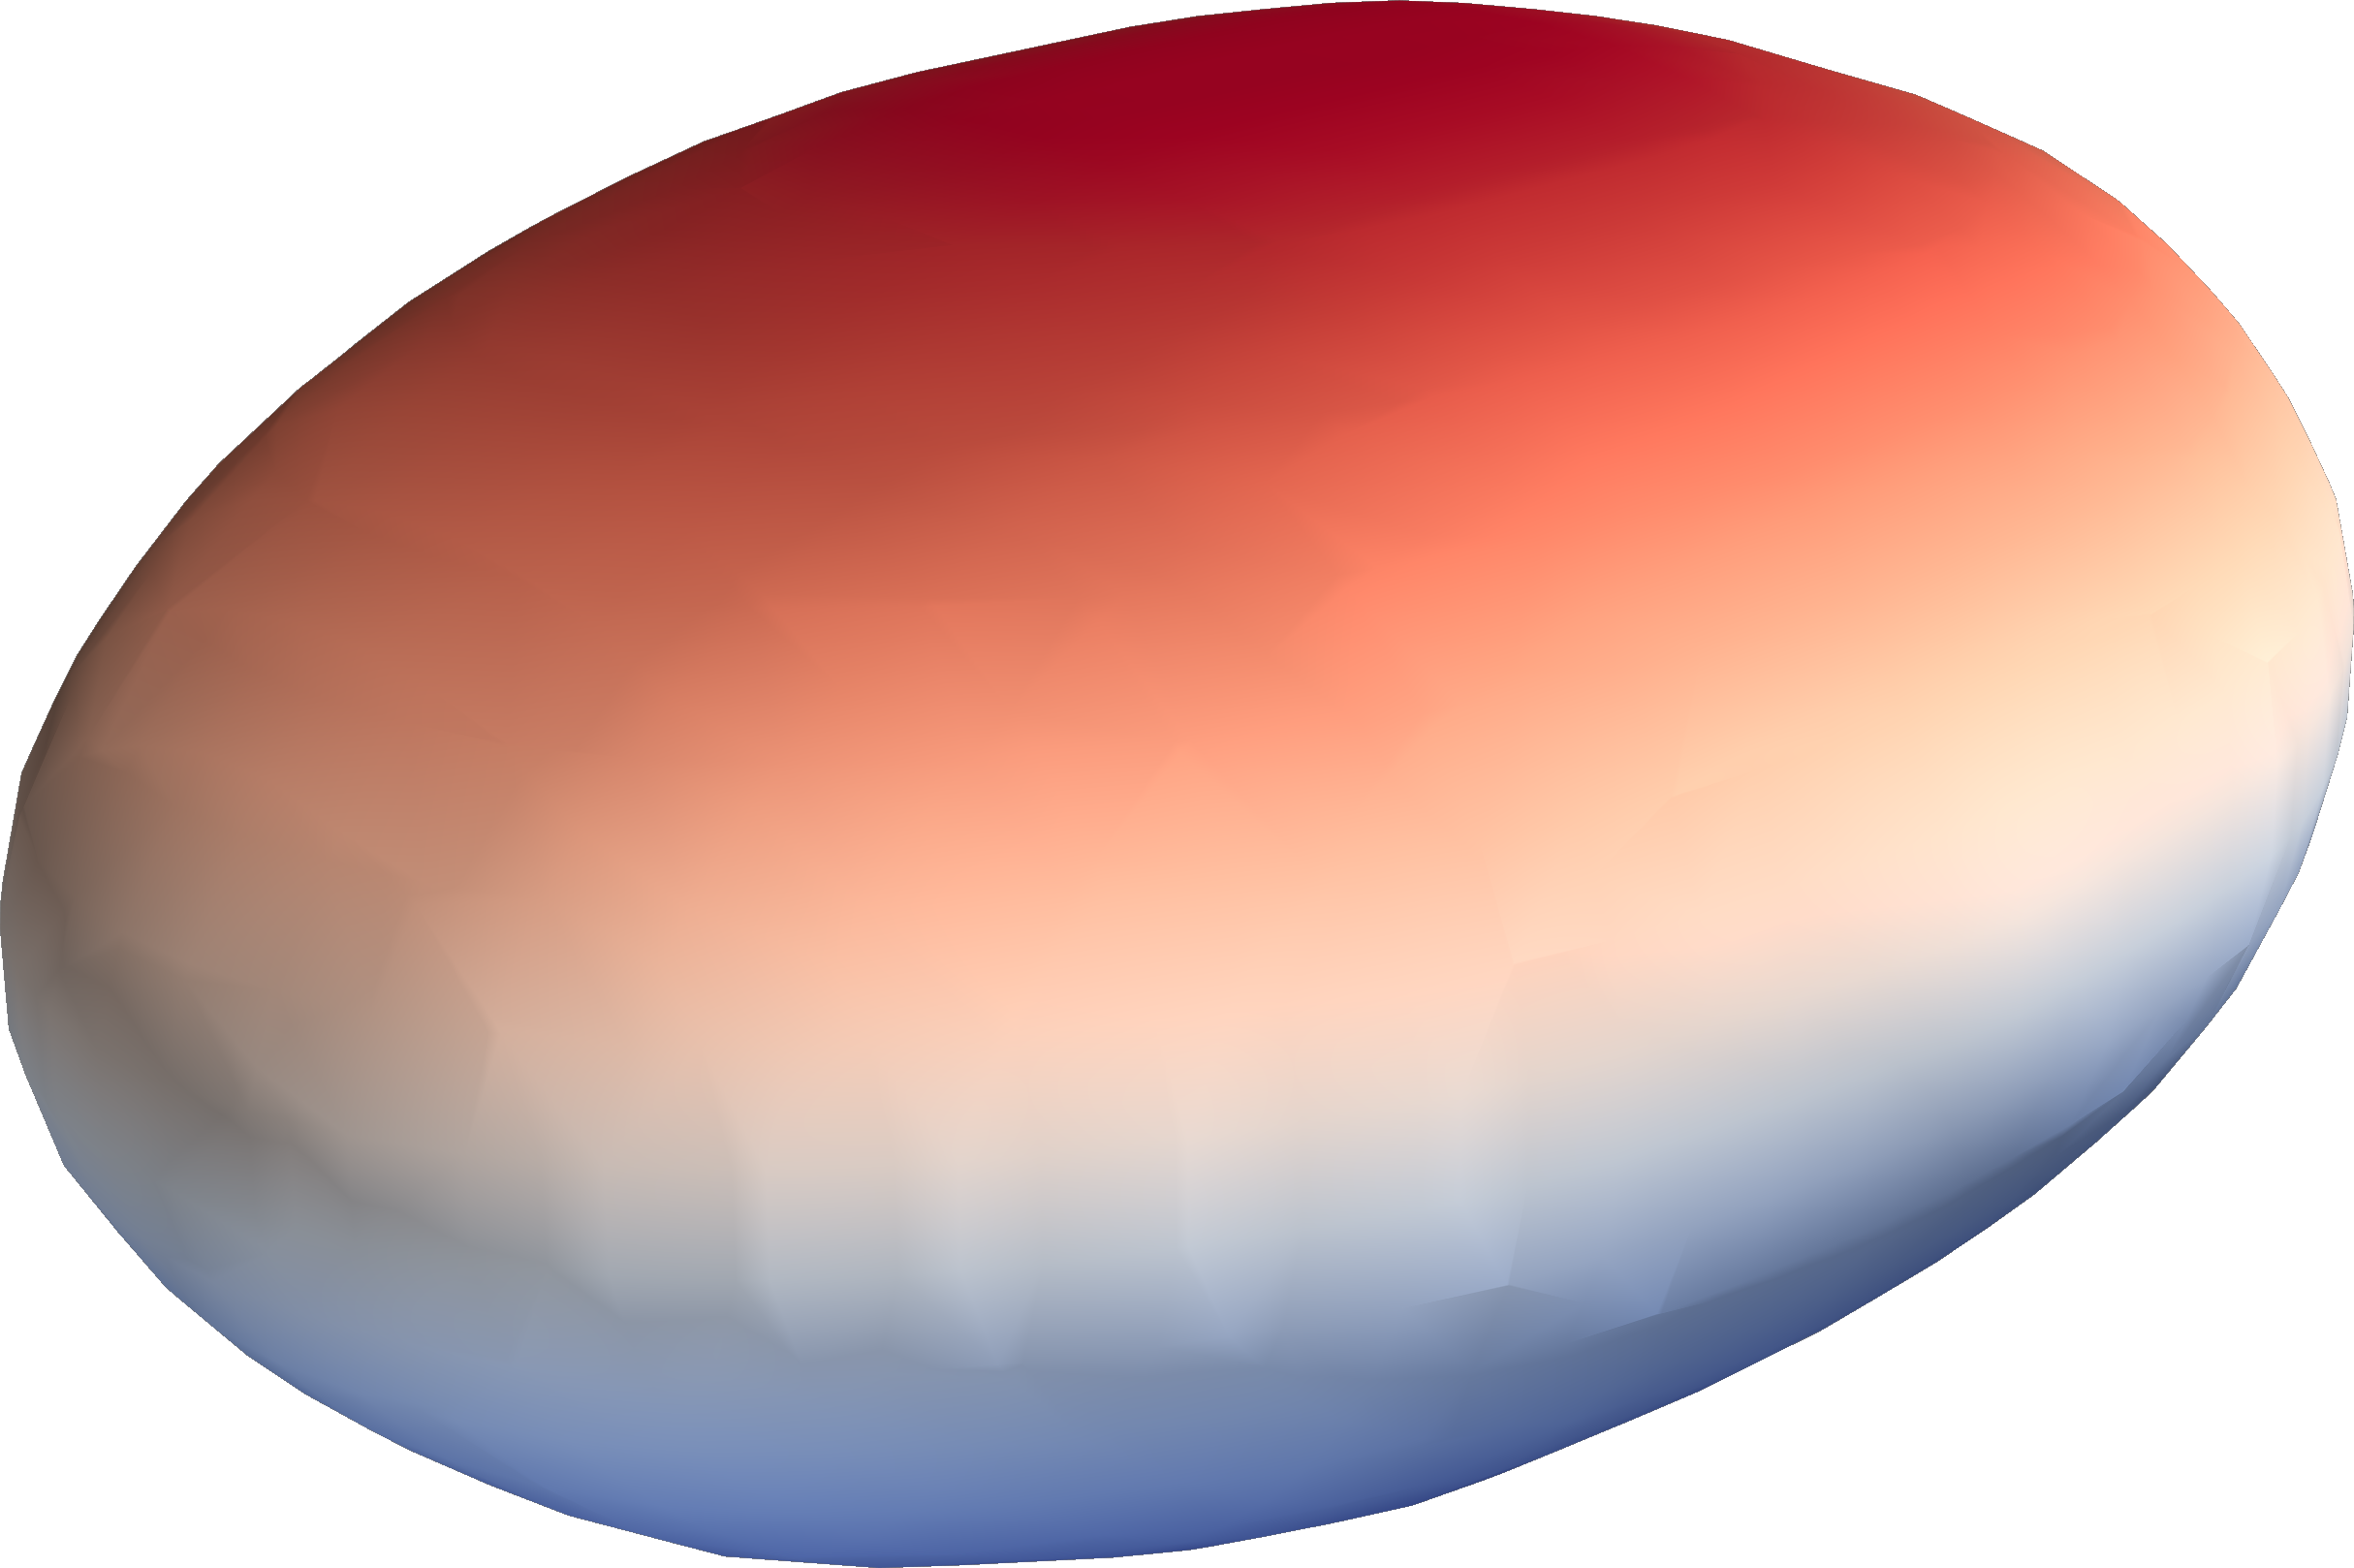
\includegraphics[width=\textwidth]{../images/3D/Ellipsoid_marching_squares_gaussian.png}
    \caption{The triangular mesh produced by marching squares.}
    \label{fig:Ellipsoid_marching_squares_gaussian}
    \end{subfigure}
    \caption{Illustration of contour interpolation using convolution with Gaussian kernel with $\sigma=2$ and kernel width of 3.}
    \label{fig:Ellipsoid_gaussian}
\end{figure}

Figure \ref{fig:Ellipsoid_gaussian} neatly demonstrates the power of the Gaussian filter. Even with kernel width of only $3$, the resulting contour mesh is very smooth. Increasing the kernel width (alongside with $\sigma$) will increase the smoothness even further, but it doesn't come without expenses. Large $\sigma$ will cause very small or very thin regions to disappear completely, as the $1$s will be diffused into the surrounding $0$s, likely bringing their values under $0.5$, meaning that the marching squares algorithm will not notice these as the interior of the object.

\section{Applying Gaussian Filter to Simulation Data}\label{sec:simulation}
The goal of comparing various ways to produce a smooth contour from 3D binary data was to apply one of the techniques to real simulation data. The data referenced here is produced by simulating closed and open flux coronal magnetic fields.\footnote{\url{https://doi.org/10.3847/1538-4357/ac5d5b}} The isosurface in the following figures represent the boundaries between the regions of open and closed flux magnetic fields.
\begin{figure}[H]
    \centering
    \begin{subfigure}{.49\textwidth}
        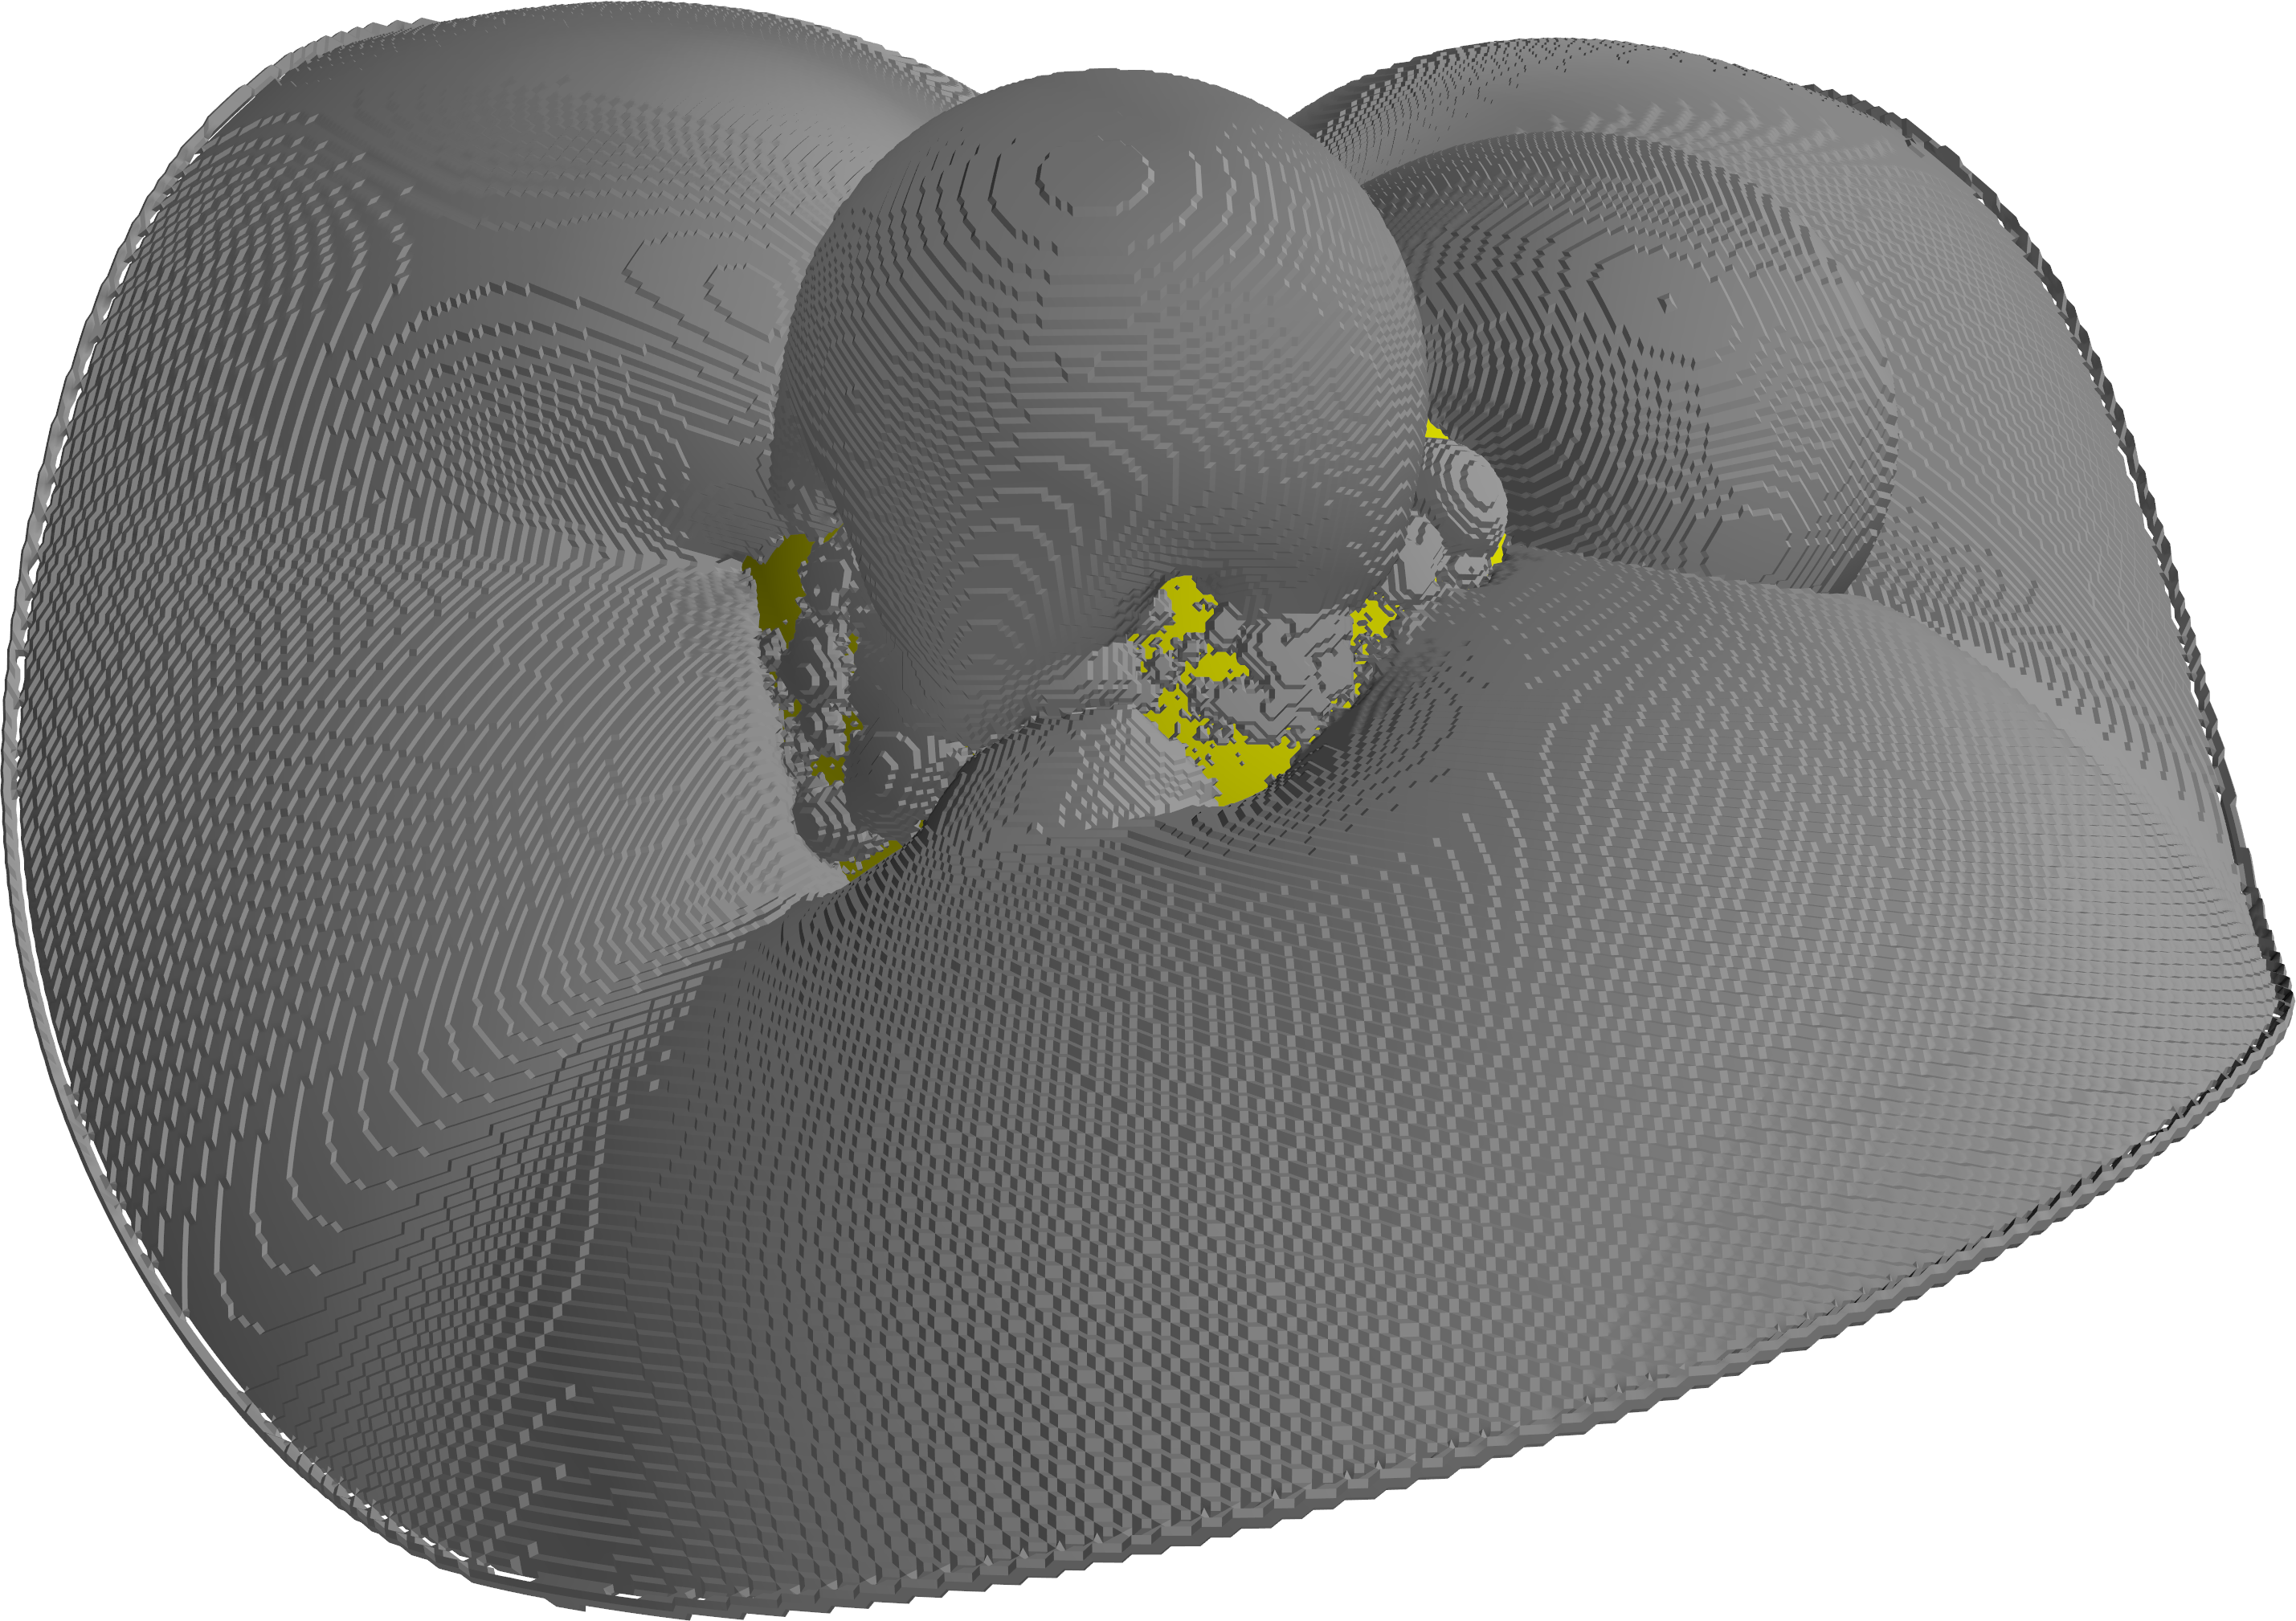
\includegraphics[width=\textwidth]{../images/3D/Dataset1.png}
    \caption{An isosurface produced from the data by applying marching squares directly.}
    \end{subfigure}
    \hfill
    \begin{subfigure}{.49\textwidth}
        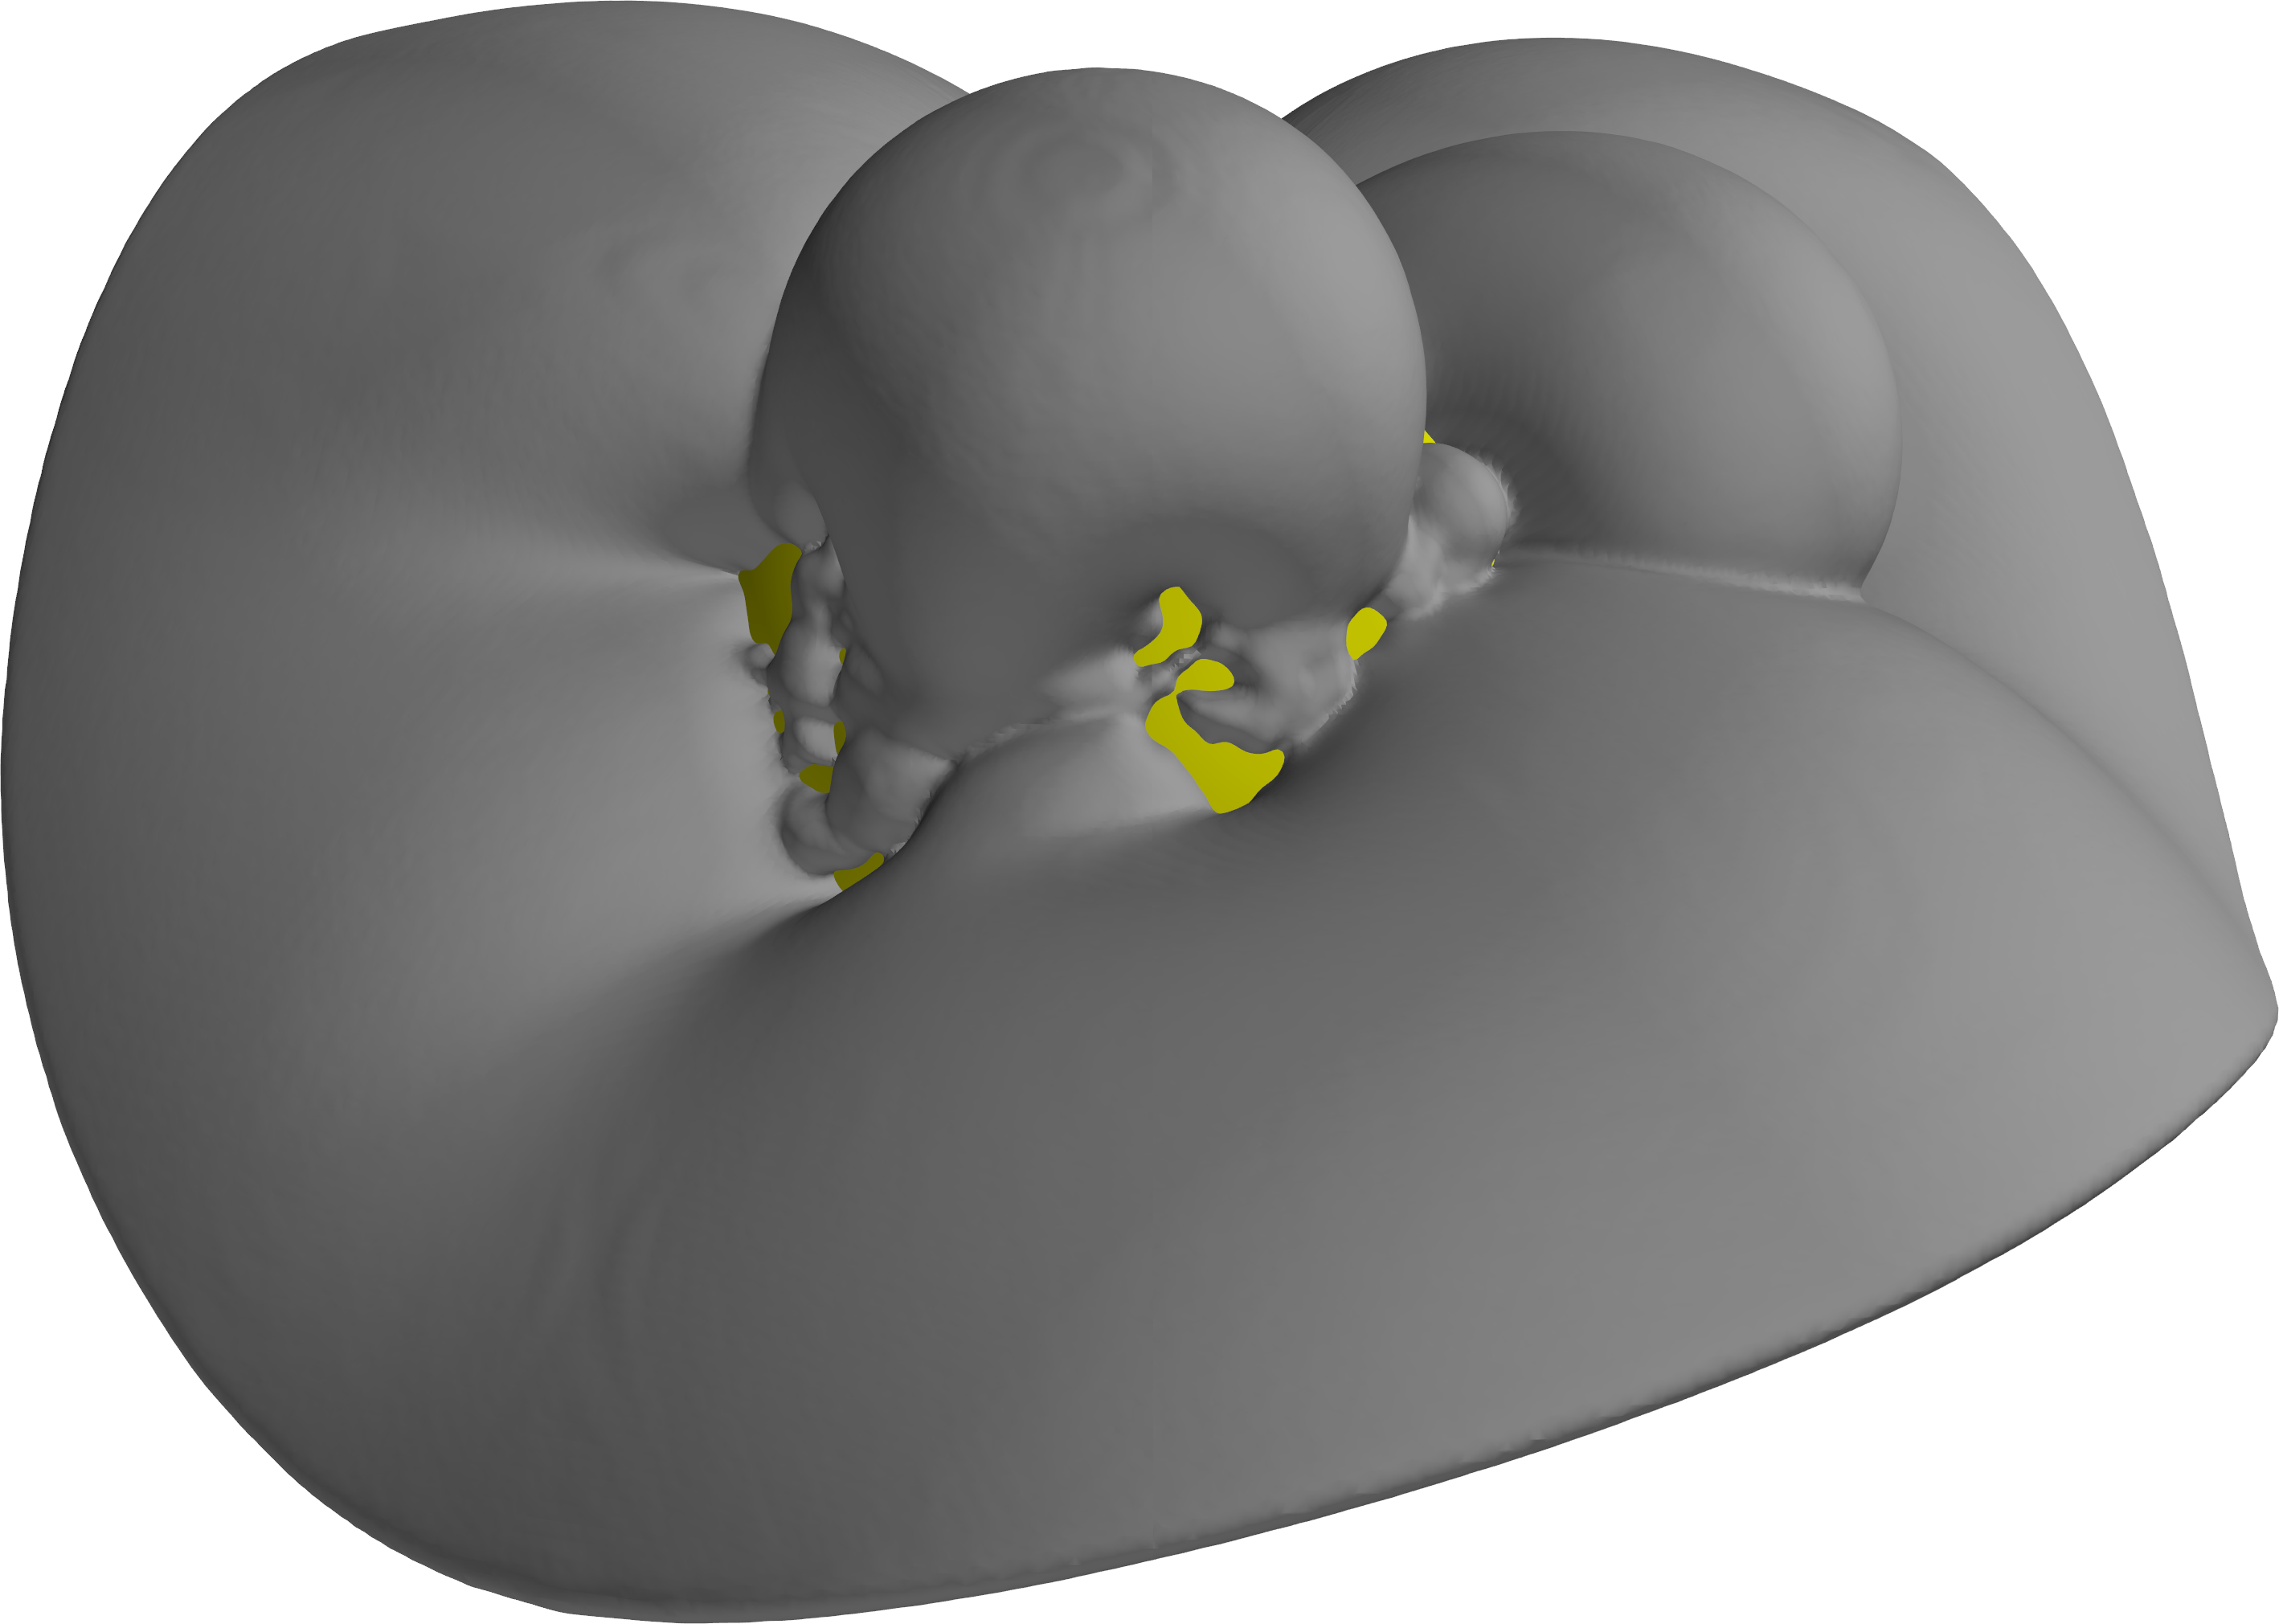
\includegraphics[width=\textwidth]{../images/3D/Dataset1_Gaussian.png}
    \caption{An isosurface produced from the data by applying marching squares after applying the Gaussian filter.}
    \end{subfigure}
    \caption{Isosurfaces from the first dataset from the simulation.}
    \label{fig:Dataset1}
\end{figure}
\begin{figure}[H]
    \centering
    \begin{subfigure}{.49\textwidth}
        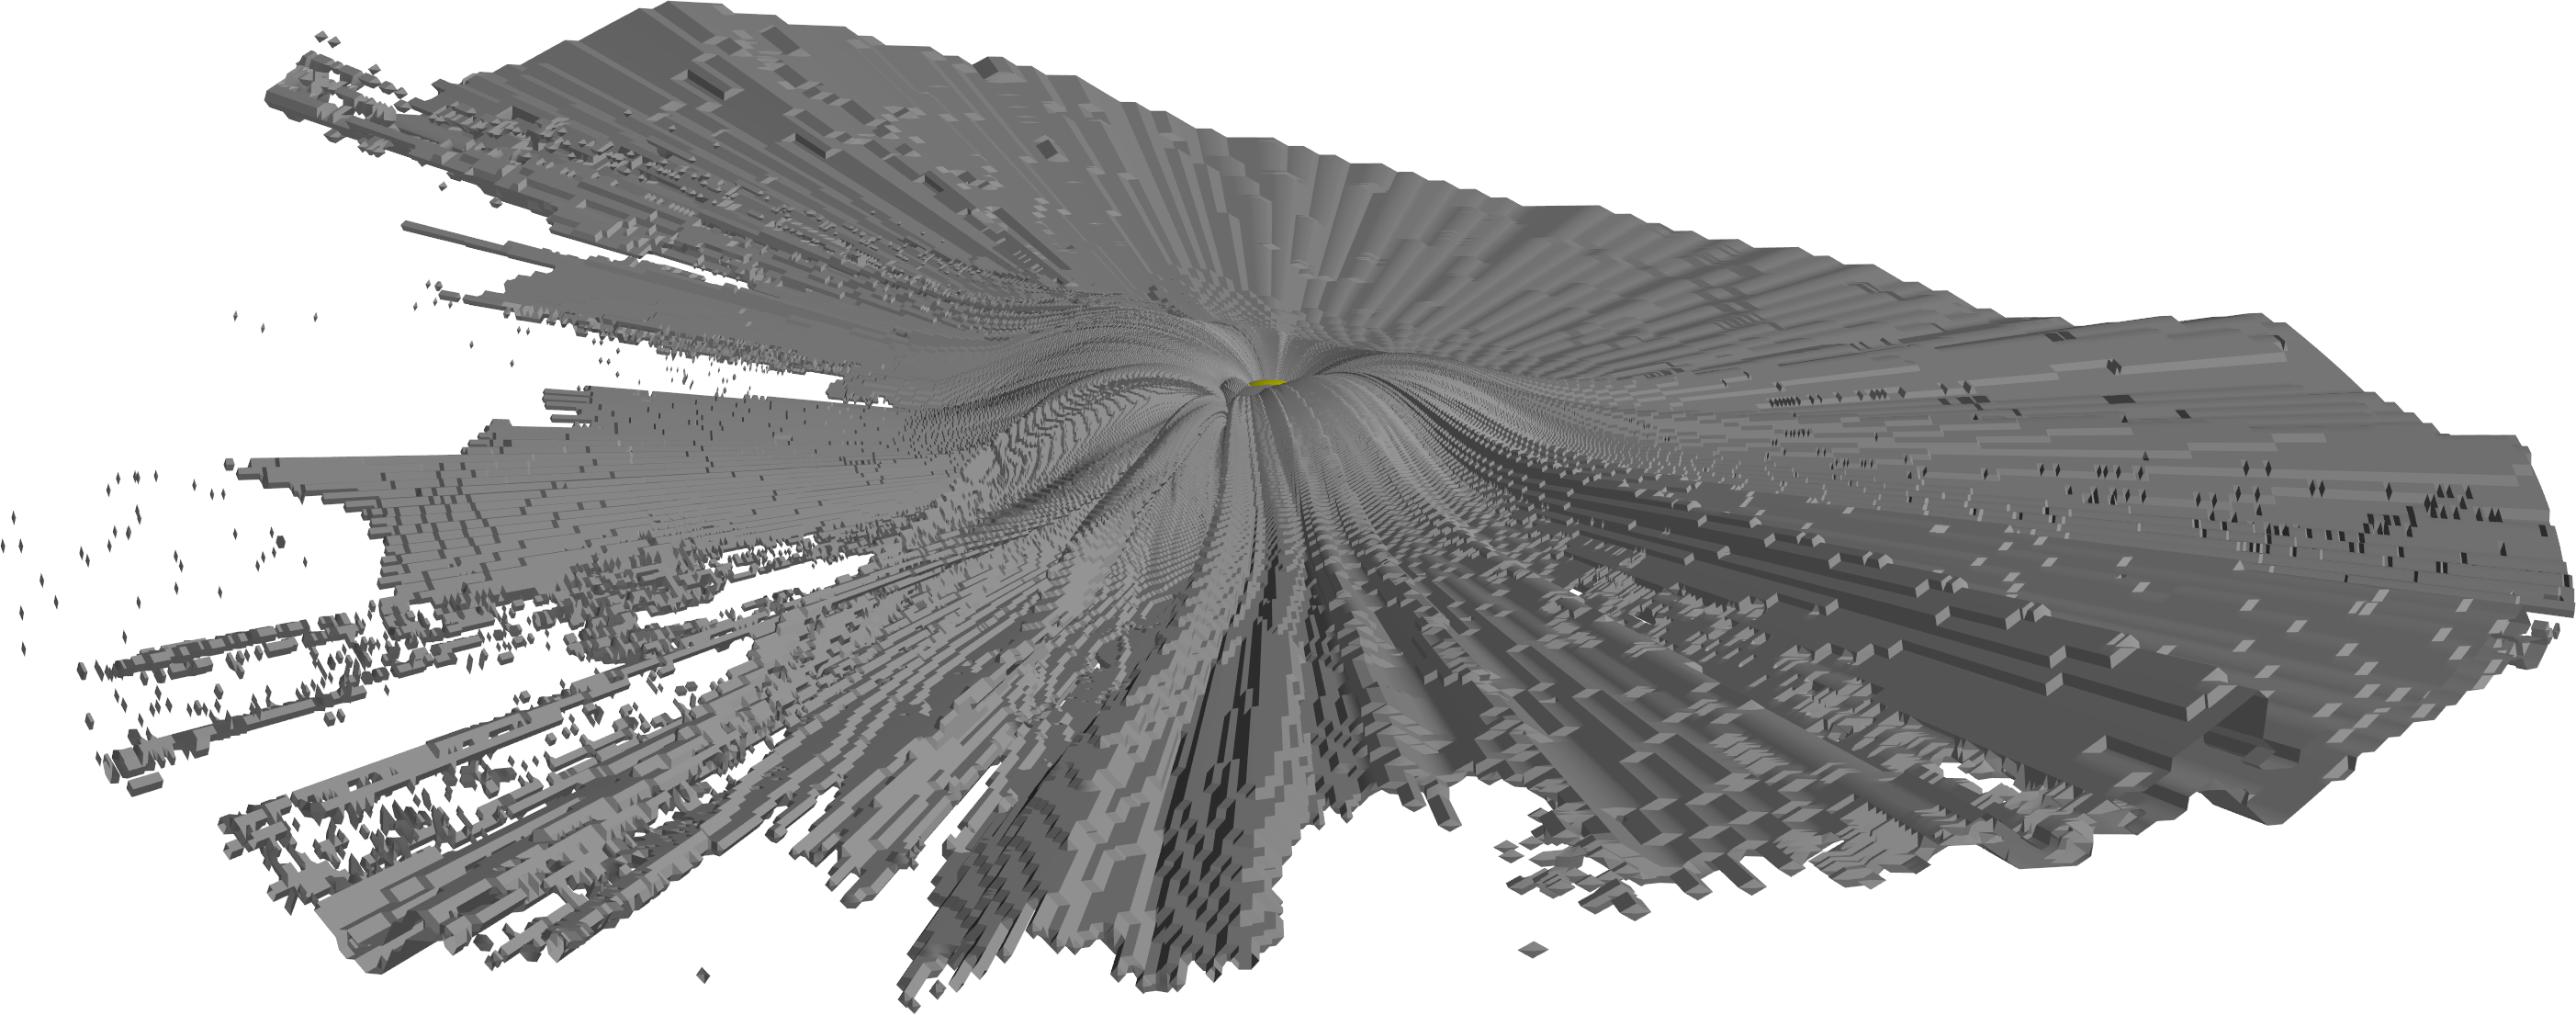
\includegraphics[width=\textwidth]{../images/3D/Dataset2.png}
    \caption{An isosurface produced from the data by applying marching squares directly.}
    \end{subfigure}
    \hfill
    \begin{subfigure}{.49\textwidth}
        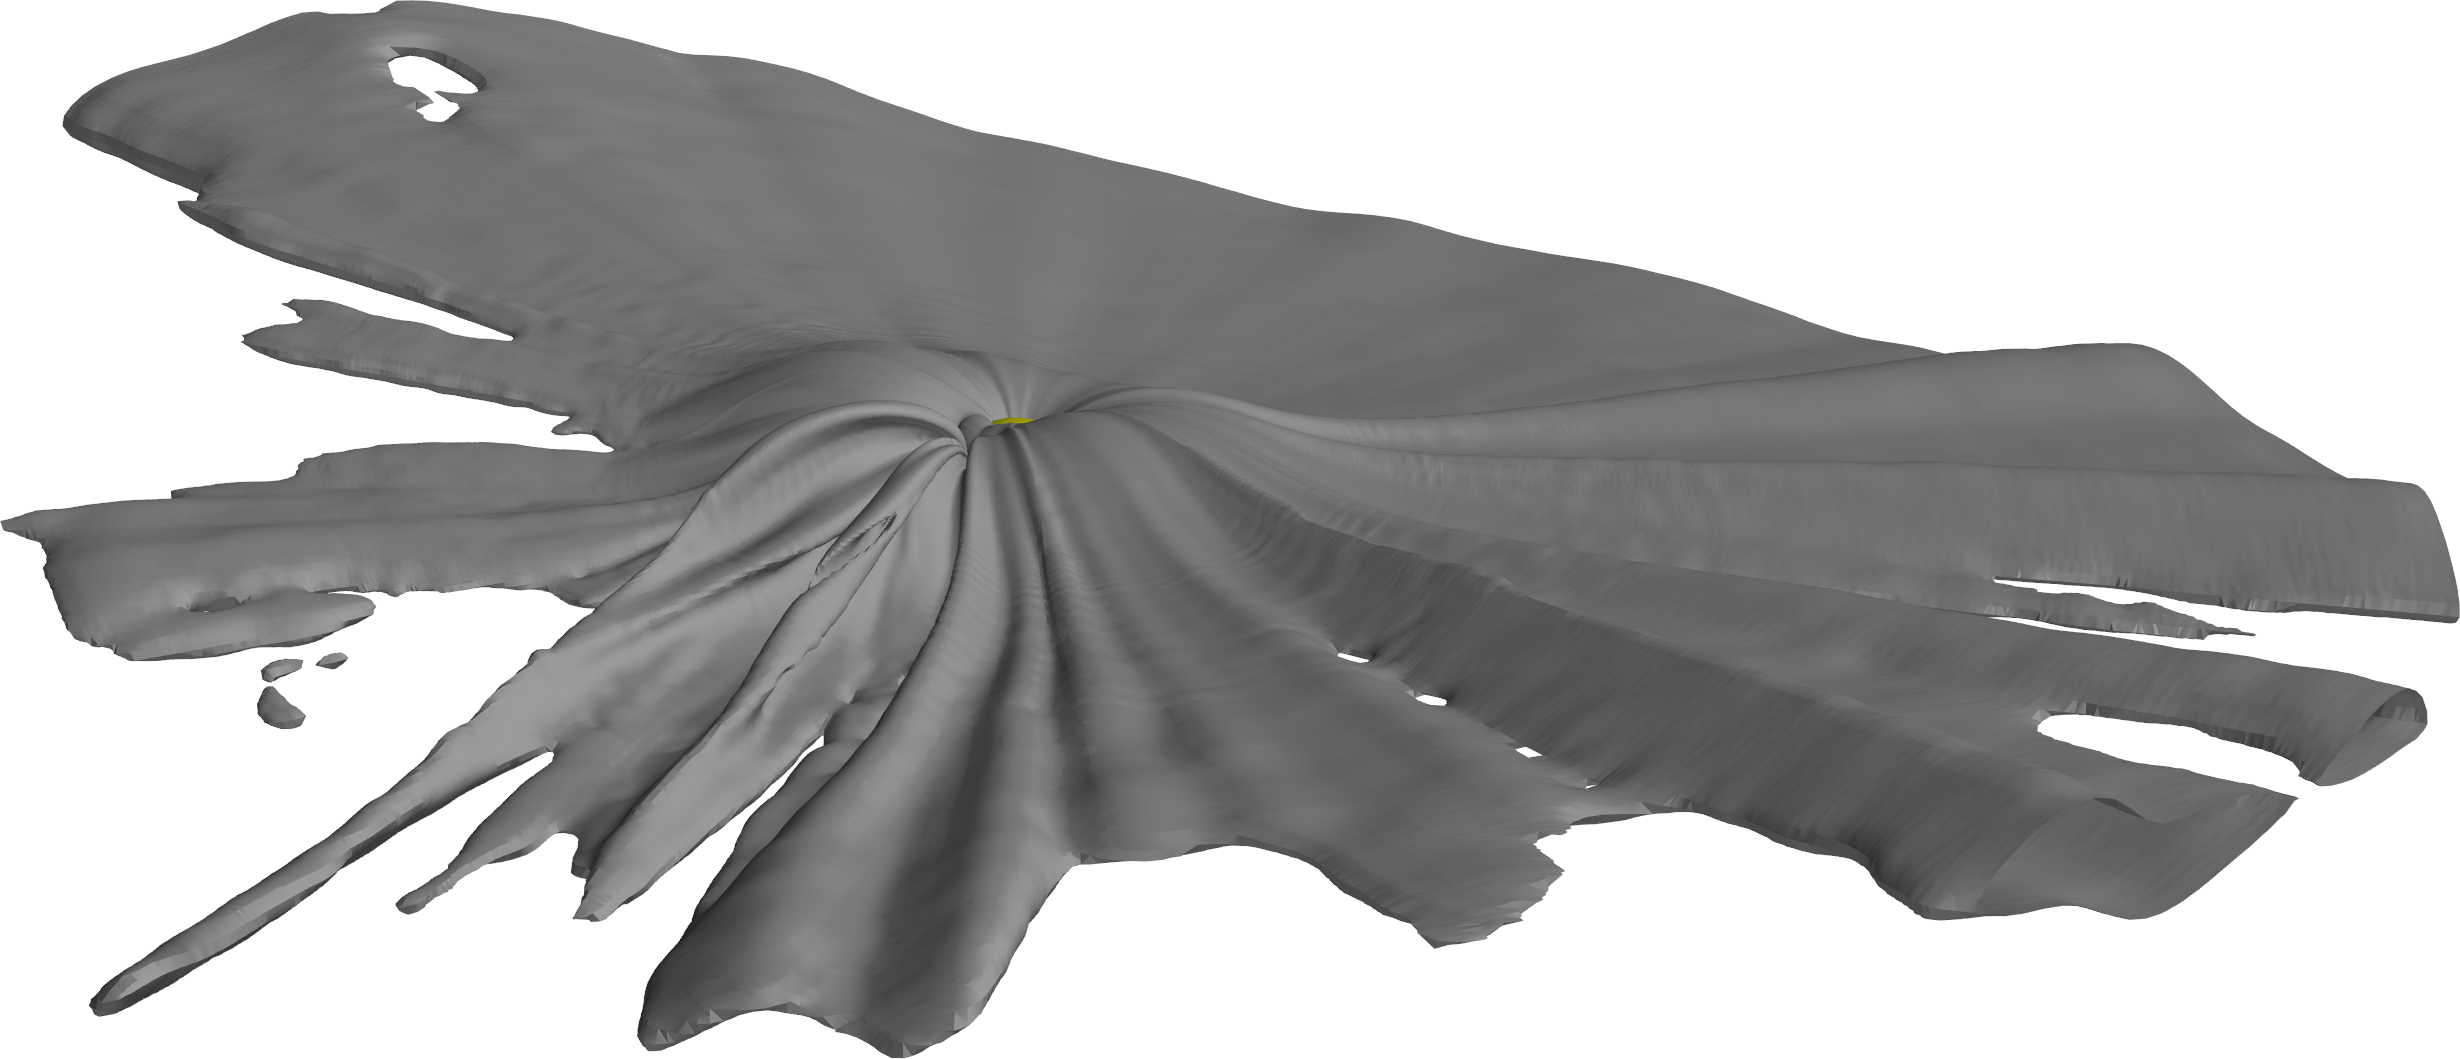
\includegraphics[width=\textwidth]{../images/3D/Dataset2_Gaussian.png}
    \caption{An isosurface produced from the data by applying marching squares after applying the Gaussian filter.}
    \end{subfigure}
    \caption{Isosurfaces from the second dataset from the simulation.}
    \label{fig:Dataset2}
\end{figure}
In both cases, the isosurface meshes were produced by applying marching squares to the data in spherical coordinate system. The Gaussian filter greatly increases the smoothness of the meshes, however as was mentioned in Section \ref{sec:gaussian_kernel}, the regions where $1$s are sparse disappeared from the mesh. This can especially be seen in Figure \ref{fig:Dataset2}, where the noise from the bottom-left region does not go through to the smooth contour.

\chapter{Creating Visualizations in Unity}\label{chap:Unity}
The figures in Section \ref{sec:simulation} were all created using Python library Mayavi. The library is good for quickly visualizing 3D objects, but further adjustment of the visuals of the produced figures is quite difficult. We have decided to utilize Unity to create more visually appealing images and animations.

Importing the meshes from Python to Unity can be done in several ways, as Unity supports importing a wide range of file types. However, the mesh needs to be adjusted first to match Unity's axes orientation. Unity uses the \textit{y} axis as the \textit{up} axis, so if the original data used the \textit{z} axis as the \textit{up} axis, these two axis need to be swapped first and then the \textit{z} axis needs to be reversed (i.e. reflect all the points in the \textit{x-y} plane).

After the meshes are imported, any of the tools available in Unity can be used to change the visuals of the meshes. In Figure \ref{fig:Dataset1_Unity} and \ref{fig:Dataset2_Unity}, we have used a force field shader to add transparency and varying colour based on the mesh face's normal vectors.

\begin{figure}[H]
    \centering
    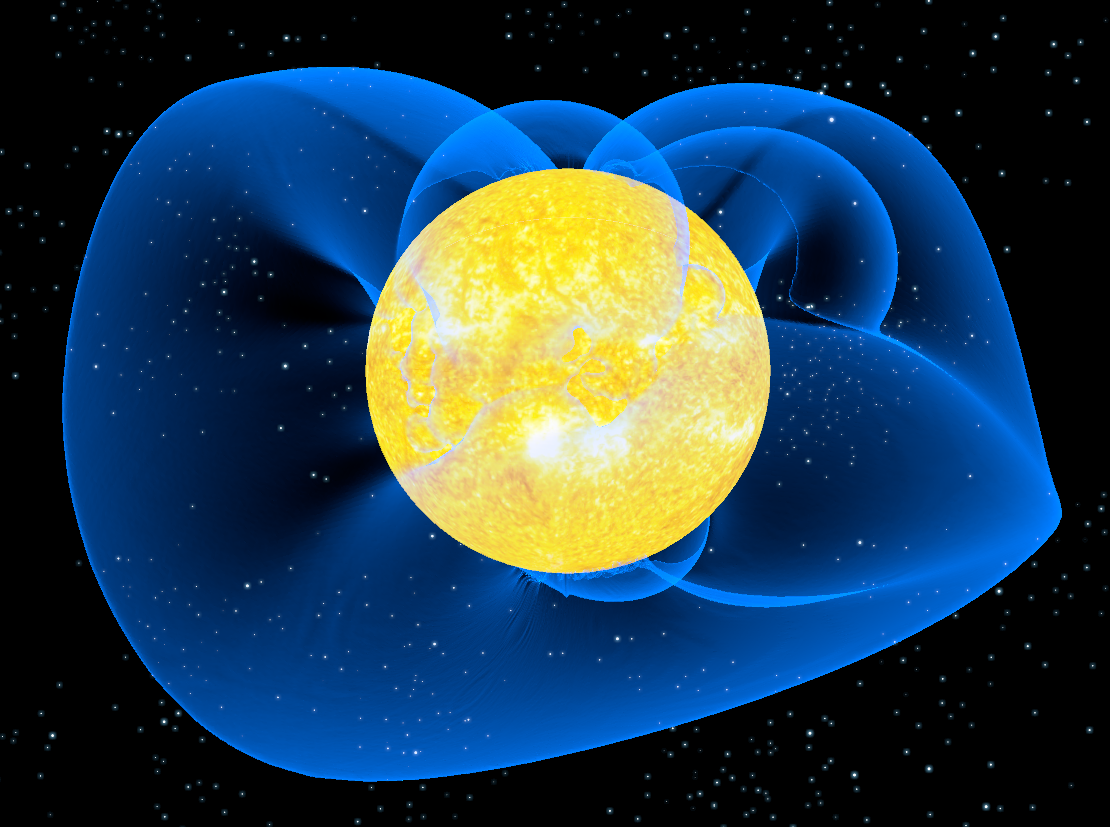
\includegraphics[width=0.7\textwidth]{../images/3D/Dataset1_Unity.png}
    \caption{The visualization of the isosurface from the first dataset.}
    \label{fig:Dataset1_Unity}
\end{figure}
\begin{figure}[H]
    \centering
    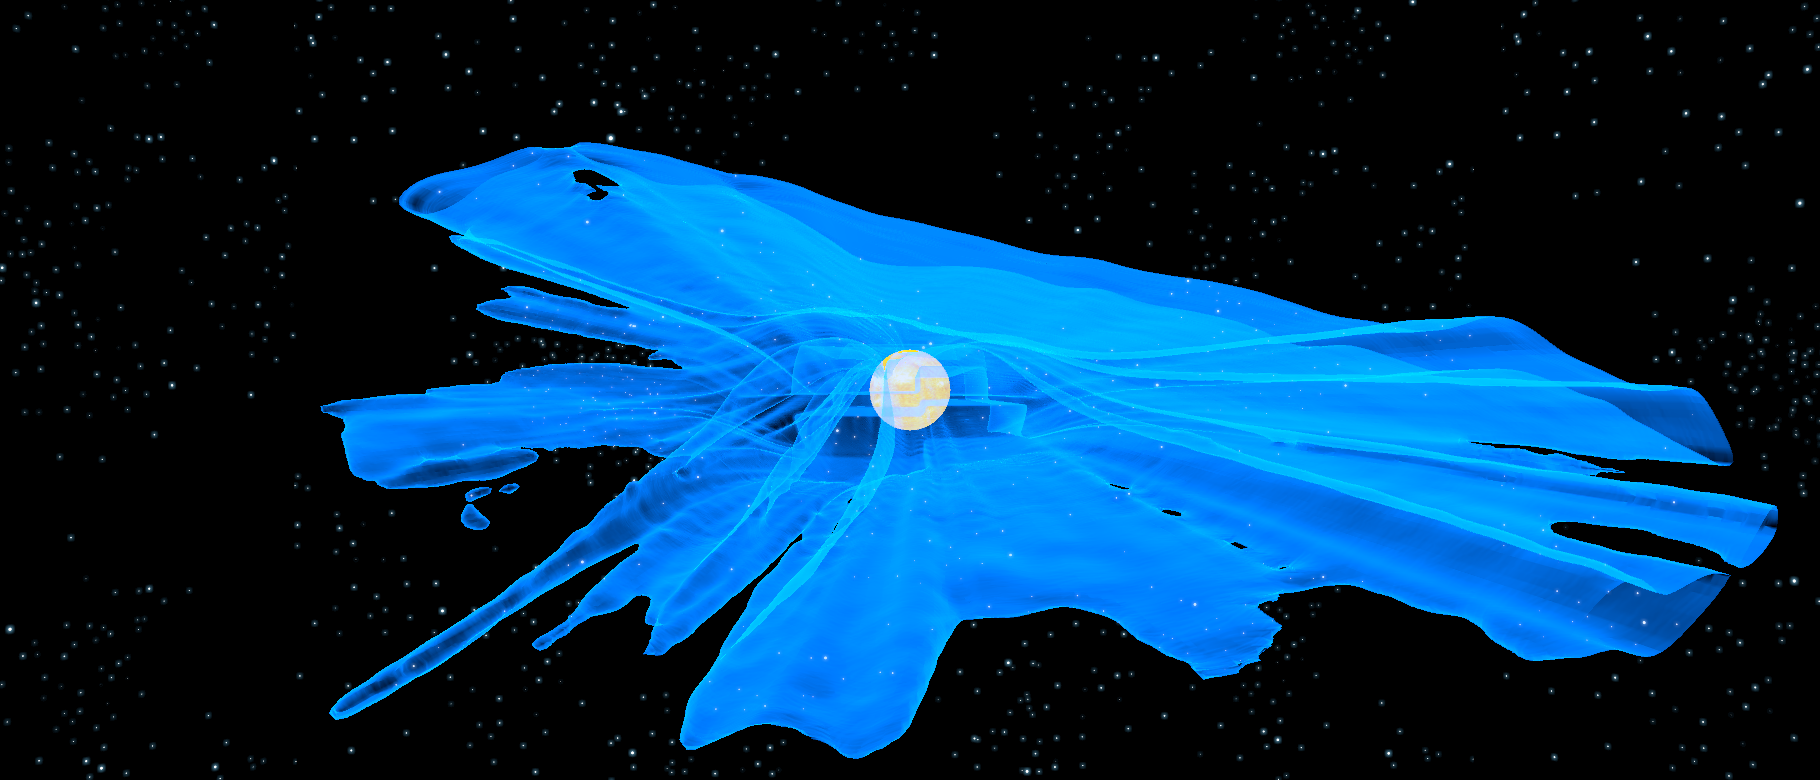
\includegraphics[width=\textwidth]{../images/3D/Dataset2_Unity.png}
    \caption{The visualization of the isosurface from the second dataset.}
    \label{fig:Dataset2_Unity}
\end{figure}
\end{document}
